\documentclass[a4paper, oneside, dvipsnames, table]{article}
\usepackage{../../Utilita/Stiletemplate}
\usepackage{hyperref}
\usepackage{fancyhdr}
\usepackage{ifthen}
\usepackage{comment}
\usepackage{enumitem}
\usepackage[italian]{babel}
\usepackage[utf8]{inputenc}
\usepackage[parfill]{parskip}

\newcommand{\Data}{2021\_01\_30}

\newcommand{\Titolo}{Verbale riunione \Data}

\newcommand{\Redattori}{\TL}

\newcommand{\Verificatori}{\PC}

\newcommand{\Approvatore}{\VD}

\newcommand{\Distribuzione}{\VT{} \newline \CR{} \newline Gruppo \Gruppo}

\newcommand{\Uso}{Interno}

\newcommand{\DescrizioneDoc}{Questo documento si occupa di riportare quanto discusso nella riunione del \Data.}

\newcommand{\pathimg}{../../../Immagini/N.O.S.jpg}

\newcommand{\Versionedoc}{1.0}
% info generali 
\newcommand{\NomeProgetto}{\textit{Emporio$\lambda$ambda}}

% fornitore
\newcommand{\Gruppo}{\textit{N.O.S}}
\newcommand{\Mail}{nos.unipd@gmail.com}

% committenti
\newcommand{\Committente}{\VT \newline \CR}
\newcommand{\VT}{Prof. Vardanega Tullio}
\newcommand{\CR}{Prof. Cardin Riccardo}

% proponenti
\newcommand{\Proponente}{\textit{RedBabel}}

% Componenti
\newcommand{\BL}{Brescanzin Lorenzo}
\newcommand{\FF}{Fantinato Filippo}
\newcommand{\MM}{Martini Matteo}
\newcommand{\PC}{Panighel Cristiano}
\newcommand{\TG}{Terrani Giulia}
\newcommand{\TL}{Tredese Leonardo}
\newcommand{\VD}{Varotto Davide}

% ruoli

\newcommand{\Responsabile}{\textit {Responsabile di Progetto}}
\newcommand{\Amministratore}{\textit{Amministratore di Progetto}}

% documenti

\newcommand{\SdF}{Studio di Fattibilità}
\newcommand{\SdFv}[1]{\textit{Studio di Fattibilità {#1}}}
\newcommand{\PdQ}{Piano di Qualifica}
\newcommand{\PdQv}[1]{\textit{Piano di Qualifica {#1}}}
\newcommand{\PdP}{Piano di Progetto}
\newcommand{\PdPv}[1]{\textit{Piano di Progetto {#1}}}
\newcommand{\NdP}{Norme di Progetto}
\newcommand{\NdPv}[1]{\textit{Norme di Progetto {#1}}}
\newcommand{\AdR}{Analisi dei Requisiti}
\newcommand{\AdRv}[1]{\textit{Analisi dei Requisiti {#1}}}
\newcommand{\Glossario}{Glossario}
\newcommand{\Glossariov}[1]{\textit{Glossario {#1}}}

% comandi generali
\newcommand{\glo}[1]{#1\ap{G}}

\newcommand{\myparagraph}[1]{\paragraph{#1}\mbox{}\\}

\setcounter{tocdepth}{5}  \setcounter{secnumdepth}{5}


\begin{document}

\copertina
\fancydoc

\registroModifiche{
	
	2.0 & 2021\_03\_06 & \VD{} & Responsabile & - & Approvazione del documento. \\
	
	1.20 & 2021\_03\_05 & \MM{} & Analista & \TL{} & Inseriti UML corretti. \\
	
	1.19 & 2021\_03\_04 & \PC{} & Analista & \TL{} & Aggiornata sezione \S\ref{Tracciamento}. \\
	
	1.18 & 2021\_03\_02 & \PC{} & Analista & \BL{} & Aggiornata sezione \S\ref{ReqFunz}, requisiti del venditore. \\
	
	1.17 & 2021\_03\_01 & \MM{} & Analista & \PC{} & Aggiornata sezione \S\ref{ReqFunz}, requisiti dell'acquirente. \\
	
	1.16 & 2021\_02\_26 & \BL{} & Analista & \PC{} & Correzione dei precedenti e aggiunta di nuovi UC, estensioni di UC già presenti. \\

	1.15 & 2021\_02\_25 & \TG{} & Analista & \PC{} & Correzione UC "Lista riepilogo ordini" ora UC\ref{visualizzazione-ordini-in-gestione} e aggiunta UC da UC\ref{modifica-stato-ordine} a UC\ref{filtro-ordini-venditore}. \\
	
	1.14 & 2021\_02\_24 & \TG{} & Analista & \FF{} & Redatti nuovi UC\ref{ricerca-codice-ordine-acquirente} e UC\ref{filtro-temporale-ordini-acquirente}.\\
	
	1.13 & 2021\_02\_21 & \TG{} & Analista & \FF{} & Redatti nuovi UC\ref{inserimento-indirizzo-consegna}, UC\ref{modifica-indirizzo-consegna} e UC\ref{eliminazione-indirizzo-consegna}. \\
	
	1.12 & 2021\_02\_19 & \MM{} & Analista & \TG{} & Eliminato UC23-"Inserimento campo dati" e UC15-"Modifica informazioni profilo" ora suddiviso in UC\ref{modifica-informazioni-acquirente} e UC\ref{modifica-informazioni-venditore}. \\

	1.11 & 2021\_02\_18 & \PC{} & Analista & \BL{} & Correzione UC\ref{checkout}. \\

	1.10 & 2021\_02\_15 & \BL{} & Analista & \PC{} & Correzioni \S\ref{ReqVincolo} e \S\ref{ReqQual}, da UC\ref{aggiunta-carrello-plp} a UC\ref{modifica-quantita-nel-carrello}.\\
	
	1.9 & 2021\_02\_14 & \BL{} & Analista & \TG & Sistemazione UC\ref{logout} e UC\ref{ricerca-prodotti-acquirente}. \\
	
	1.8 & 2021\_02\_13 & \TG{} & Analista & \MM{} & Aggiunto i casi d'uso UC\ref{aggiunta-categoria}, UC\ref{modifica-categoria}, UC\ref{eliminazione-categoria}. \\

	1.7 & 2021\_02\_10 & \PC{} & Analista & \MM{} & Corretto i caso d'uso UC\ref{aggiunta-prodotto-evidenza} e UC\ref{rimozione-prodotto-evidenza}. \\

	1.6 & 2021\_02\_09 & \TG{} & Analista & \TL{} & Corretto le sezioni UC\ref{aggiunta-prodotto} e UC\ref{modifica-prodotto}. \\
	
	1.5 & 2021\_02\_08 & \MM{} & Analista & \FF{} & Trasformato sottocasi d'uso indipendenti relativi al venditore in casi d'uso. \\
	
	1.4 & 2021\_02\_04 & \MM{} & Analista & \PC{} & Trasformato sottocasi d'uso indipendenti relativi all'acquirente in casi d'uso. \\

	1.3 & 2021\_02\_03 & \TG{} & Analista & \TG{} & Rimossi i dettagli implementativi dai casi d'uso. Eliminato UC3-"Accesso al menù". \\

	1.2 & 2021\_02\_02 & \PC{} & Analista & \TL{} & Separati i casi di accesso alla piattaforma sezione \S\ref{AccessoPiattaforma}. \\

	1.1 & 2021\_02\_02 & \BL{} & Analista & \FF{} & Rimosso l'attore amministratore sezione \S\ref{Attori}. \\ 

	1.0.0 & 2021\_01\_10 & \PC{} & Responsabile & - & Approvazione del documento. \\
	
	0.1.7 & 2021\_01\_09 & \FF{} & Analista & \TL{} & Stesura riepilogo tracciamento \S\ref{Riepilogo} \\
	
	0.1.6 & 2021\_01\_09 & \TL{} & Analista & \BL{} & Stesura tracciamento requisito-fonte \S\ref{ReqFonte} \\
	
	0.1.5 & 2021\_01\_09 & \BL{} & Analista & \FF{} & Stesura tracciamento fonte-requisito \S\ref{FonteReq} \\
	
	0.1.4 & 2021\_01\_08 & \MM{} & Analista & \BL{} & Aggiunta diagrammi dei casi d'uso \S\ref{CasiUso} \\
	
	0.1.3 & 2021\_01\_08 & \TL{} & Analista & \TG{} & Stesura requisiti vincolo \S\ref{ReqVincolo} e prestazionali \S\ref{ReqPrest} \\
	
	0.1.2 & 2021\_01\_08 & \FF{} & Analista & \TG{} & Stesura requisiti di qualità \S\ref{ReqQual} \\
	
	0.1.1 & 2021\_01\_07 & \BL{} & Analista & \TG{} & Stesura requisiti funzionali \S\ref{ReqFunz} \\
	
	0.1.0 & 2021\_01\_06 & - & - & \TG{} & Verifica complessiva del documento. \\
	
	0.0.10  & 2020\_12\_27 & \FF{} & Analista & \TG{} & Stesura caso d'uso UC\ref{estensione:limite-foto-raggiunto}, UC\ref{estensione:prezzo-minore-o-uguale-zero}, UC\ref{estensione:email-non-esistente}, UC\ref{estensione:registrazione-con-email-non-esistente}, UC\ref{estensione:quantita-da-aggiungere-al-carrello-non-valida}, UC\ref{estensione:sconto-minore-zero}, UC\ref{estensione:pagamento-fallito}, UC\ref{estensione:sconto-maggiore-cento} \\
	
	0.0.9 & 2021\_01\_05 & \BL{} & Analista & \TG{} & Stesura casi d'uso: UC\ref{estensione:cambio-con-email-esistente}, UC\ref{estensione:campo-obbligatorio-non-inserito}, UC\ref{estensione:credenziali-non-presenti}, UC\ref{estensione:email-non-valida}, UC\ref{estensione:file-no-tipo-immagine} \\
	
	0.0.8 & 2021\_01\_04 & \TL{} & Analista & \TG{} & Aggiornamento sezioni UC\ref{eliminazione-prodotto}, UC\ref{aggiunta-prodotto-evidenza}, UC\ref{rimozione-prodotto-evidenza}, UC\ref{rifornimento-prodotto} \\
	
	0.0.7 & 2021\_01\_04 & \TL{} & Analista & \TG{} & Aggiornamento sezioni UC\ref{modifica-informazioni-venditore}, UC\ref{eliminazione-account-acquirente}, UC\ref{aggiunta-prodotto}, UC\ref{modifica-prodotto} e \S\ref{Attori} \\
	
	0.0.6 & 2021\_01\_03 & \BL{} & Analista & \TG{} & Stesura casi d'uso: UC\ref{modifica-quantita-da-aggiungere-al-carrello}, UC\ref{eliminazione-prodotto-dal-carrello}, UC\ref{checkout}, UC\ref{visualizzazione-ordini-effettuati}, UC\ref{modifica-informazioni-acquirente} \\
	
	0.0.5  & 2021\_01\_02 & \BL{} & Analista & \TG{} & Stesura casi d'uso: UC\ref{ordinamento-prezzo-decrescente}, UC\ref{aggiunta-carrello-pdp}, UC\ref{aggiunta-carrello-plp} \\
	
	0.0.4  & 2021\_01\_02 & \FF{} & Analista & \TG{} & Stesura casi d'uso: UC\ref{logout}, UC\ref{ricerca-prodotti-acquirente}, UC\ref{filtro-prodotti-acquirente}, UC\ref{ordinamento-prezzo-crescente} \\
	
	0.0.3  & 2021\_01\_01 & \FF{} & Analista & \TG{} & Stesura casi d'uso: UC\ref{registrazione}, UC\ref{autenticazione-acquirente}, UC\ref{autenticazione-venditore}, UC\ref{password-dimenticata} \\ 
	
	0.0.2  & 2020\_12\_27 & \TG{} & Analista & \TL{} & Stesura \S\ref{Desc} \\  
	
	0.0.1  & 2020\_12\_22 & \TG{} & Analista & \BL{} & Stesura scheletro del documento, \S\ref{Intro}, \S\ref{Desc} \\
}


\clearpage
\tableofcontents
\clearpage
\listoffigures
\clearpage
\listoftables
\clearpage

\section{Introduzione}
\subsection{Scopo del Documento}
Questo documento contiene la stesura dello studio di fattibilità riguardante i sette capitolati proposti, elencando quelli che il nostro gruppo ha considerato come i loro aspetti più interessanti e le loro criticità. Infine, per ogni capitolato vengono esposte le motivazioni e le ragioni per cui il gruppo ha scelto come progetto il capitolato C2 \NomeProgetto{} a discapito degli altri sei proposti.

\subsection{Glossario}
Al fine di evitare ambiguità fra i termini, e per avere le terminologie chiare fra tutti gli stakeholder, il gruppo \Gruppo{} ha redatto un documento denominato \Glossariov{1.0.0}.
In tale documento sono presenti tutti i termini tecnici, ambigui, specifici del progetto e scelti dai membri del gruppo con le loro relative definizioni.
Un termine presente nel \Glossariov{1.0.0} e utilizzato in questo documento viene indicato con un apice \ap{G} alla fine della parola.

\subsection{Riferimenti}

\subsubsection{Normativi}
\begin{itemize}
\item \NdPv{1.0.0}.
\end{itemize}

\subsubsection{Informativi}

\begin{itemize}
\item \textbf {Capitolato d'appalto C1 - BlockCOVID:}\\
\url{https://www.math.unipd.it/~tullio/IS-1/2020/Progetto/C1.pdf}
\item \textbf {Capitolato d'appalto C2 - \NomeProgetto:}\\
\url{https://www.math.unipd.it/~tullio/IS-1/2020/Progetto/C2.pdf}
\item \textbf {Capitolato d'appalto C3 - Gathering Detection Platform:}\\
\url{https://www.math.unipd.it/~tullio/IS-1/2020/Progetto/C3.pdf}
\item \textbf {Capitolato d'appalto C4 - HD Viz:}\\
\url{https://www.math.unipd.it/~tullio/IS-1/2020/Progetto/C4.pdf}
\item \textbf {Capitolato d'appalto C5 - PORTACS:}\\
\url{https://www.math.unipd.it/~tullio/IS-1/2020/Progetto/C5.pdf}
\item \textbf {Capitolato d'appalto C6 - Realtime Gaming Platform:}\\
\url{https://www.math.unipd.it/~tullio/IS-1/2020/Progetto/C6.pdf}
\item \textbf {Capitolato d'appalto C7 - SSD:}\\
\url{https://www.math.unipd.it/~tullio/IS-1/2020/Progetto/C7.pdf}

\end{itemize}
\newpage
\section{Descrizione del prodotto} \label{Desc}
\subsection{Caratteristiche del prodotto}
Il prodotto \NomeProgetto{} commissionato da \Proponente{} consiste nello sviluppare una piattaforma generica di \glo{e-commerce} utilizzabile come prodotto illustrativo da vendere ai negozianti, sotto forma di applicazione web accessibile da browser a tre categorie di utenti: utente non autenticato, acquirente e venditore. Le necessità di business non sono solo quelle che verranno implementante durante lo svolgimento del \glo{capitolato} ma cambiano continuamente, questo significa che la piattaforma deve essere predisposta e progettata per potersi evolvere facilmente secondo le richieste dei venditori e deve essere integrabile con servizi di terze parti.

\subsection{Analisi della struttura}
La struttura del prodotto sarà divisa in:
\begin{itemize}
    \item \textbf{\glo{Front end} acquirente:} il front end dell'acquirente dovrà occuparsi di offrire un'interfaccia web utilizzabile per cercare e filtrare i prodotti, visualizzarne tutti i dettagli, visualizzare possibili sconti applicati e poterne acquistare una certa quantità. Il front end dovrà essere sviluppato con il \glo{framework} \glo{Next.js} utilizzando come linguaggio principale \glo{Typescript} e avrà il compito di occuparsi del \glo{SSR} oppure del \glo{SSG}.
    \item \textbf{Front end venditore:} il front end del venditore dovrà occuparsi di offrire un'interfaccia web utilizzabile per aggiungere, modificare e eliminare prodotti dalla piattaforma, rifornire la loro quantità se stanno per terminare, avere una panoramica su tutti gli ordini effettuati dagli utenti ed essere in grado di segnare come evaso un ordine. I requisiti tecnologici sono gli stessi del front end dell'acquirente.
    \item \textbf{\glo{Back end}:} il back end dovrà esporre i servizi della piattaforma. Dovrà essere sviluppato con tecnologia \glo{Serverless} e basato su un'architettura a \glo{microservizi}, \glo{Typescript} è il linguaggio principale da utilizzare e il rilascio avviene in \glo{AWS} con \glo{AWS Lambda} come unità di calcolo.\\
    Sarà responsabile di:
    \begin{itemize}
        \item Implementare la logica di business dell'applicazione;
        \item Gestire i dati dell'applicazione (es: ordini, informazioni utente, informazioni sul prodotto);
        \item Gestire lo stato del carrello;
        \item Integrazione con servizi di terze parti.
    \end{itemize}
    \item \textbf{Integrazione:} rappresenta tutti i servizi di terze parti integrati con il back end. A seconda del servizio di terze parti integrato con \NomeProgetto{}, il numero di ambienti di sviluppo potrà variare:
    \begin{itemize}
        \item \glo{Identity Manager} avrà \glo{Locale}, \glo{Testing} e \glo{Staging};
        \item Il servizio di pagamento avrà Testing e Staging;
        \item Il servizio \glo{CMS} (opzionale) avrà Locale, Testing e Staging.
    \end{itemize}
    \item \textbf{Monitoring:} rappresenta tutti gli strumenti utilizzati dall'amministratore per monitorare lo stato della piattaforma. Dovrà essere implementato utilizzando \glo{Amazon CloudWatch}.
    \item \textbf{Database:} rappresenta il luogo dove verranno salvati tutti i dati della piattaforma e dovrà essere sviluppato con una tecnologia integrabile con AWS.
\end{itemize}
\newpage
\section{Casi d'uso}
\label{CasiUso}

% Attori
\subsection{Attori} \label{Attori}

\begin{figure}[ht]
    \centering
    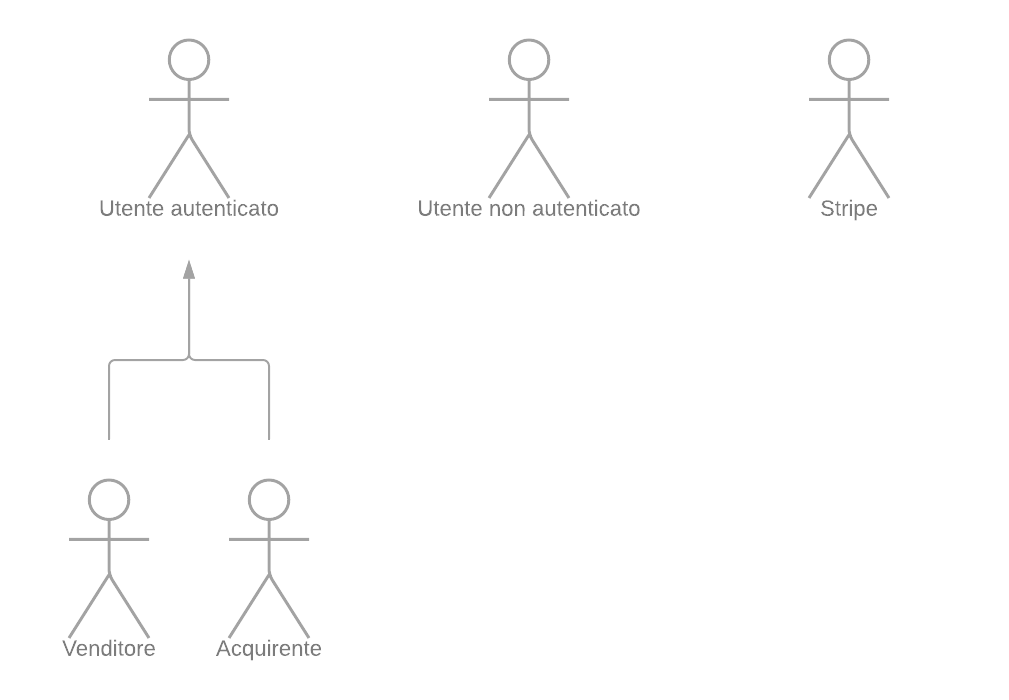
\includegraphics[width=\textwidth]{Immagini/DiagrammiUC/Attori.png}
    \caption{Gerarchia degli utenti} 
    \label{fig:Registrazione}
\end{figure}

\subsubsection{Attori Primari}
\begin{itemize}
    \item \textbf{Utente non autenticato:} utente che può consultare la parte pubblica del sito cercando prodotti e aggiungendoli al carrello, oppure fare il login o registrarsi come acquirente al sito. Non può fare però acquisti sulla piattaforma.
    \item \textbf{Utente autenticato:}
    \begin{itemize}
        \item \textbf{\glo{Acquirente}:} utente che può fare tutto ciò che fa l'utente non autenticato dopo aver effettuato la login o la registrazione. Può effettuare acquisti comprando i prodotti che ha nel carrello, consultare gli ordini che ha fatto, modificare il suo profilo e eseguire il logout.
        \item \textbf{Venditore:} utente che può aggiungere, modificare ed eliminare i prodotti dalla piattaforma, oltre a poter consultare gli ordini fatti dagli acquirenti.
    \end{itemize}
    \item \textbf{Amministratore:} l'amministratore è in grado di fare il \glo{Deploy} dell'applicazione sul \glo{cloud}, configurare le integrazioni di componenti di terze parti nella piattaforma e gestire gli utenti di tipo venditore. Questo utente non fa parte di quelli autenticati perché non svolgerà le azioni all'interno della piattaforma ma dove questa è eseguita.
\end{itemize}
\subsubsection{Attori Secondari}
\begin{itemize}
\item \textbf{\glo{Stripe}:} Servizio per la gestione di transazioni online, che verrà utilizzato per i pagamenti all'interno della piattaforma. Stripe è aderente alle normative per il pagamento online del nord America, Europa e Oceania.
\end{itemize}

% \subsection{Caratteristiche degli utenti}
% 	Acquirenti:
% 	\begin{itemize}
% 		\item Possono cercare, filtrare aggiungere al carrello come ospiti o utenti autorizzati.
% 		\item Se autenticati possono aggiornare e modificare il loro profilo.
% 		\item Creare o eliminare il proprio account
% 		\item Procedere al pagamento dei prodotti selezionati solo dopo l'autenticazione
% 	\end{itemize}
% 	Venditori:
% 	\begin{itemize}
% 		\item Visione complessiva di tutti gli ordini effettuati
% 		\item Aggiungere, rimuovere o modificare le informazioni di prodotto
% 	\end{itemize}
% 	Amministratori:
% 	\begin{itemize}
% 		\item Lanciare l'applicazione sul cloud
% 		\item Gestire la configurazione di servizi di terze parti
% 	\end{itemize}


% Riepilogo casi d'uso
\subsection{Riepilogo dei casi d'uso}

\begin{figure}[H]
    \centering
    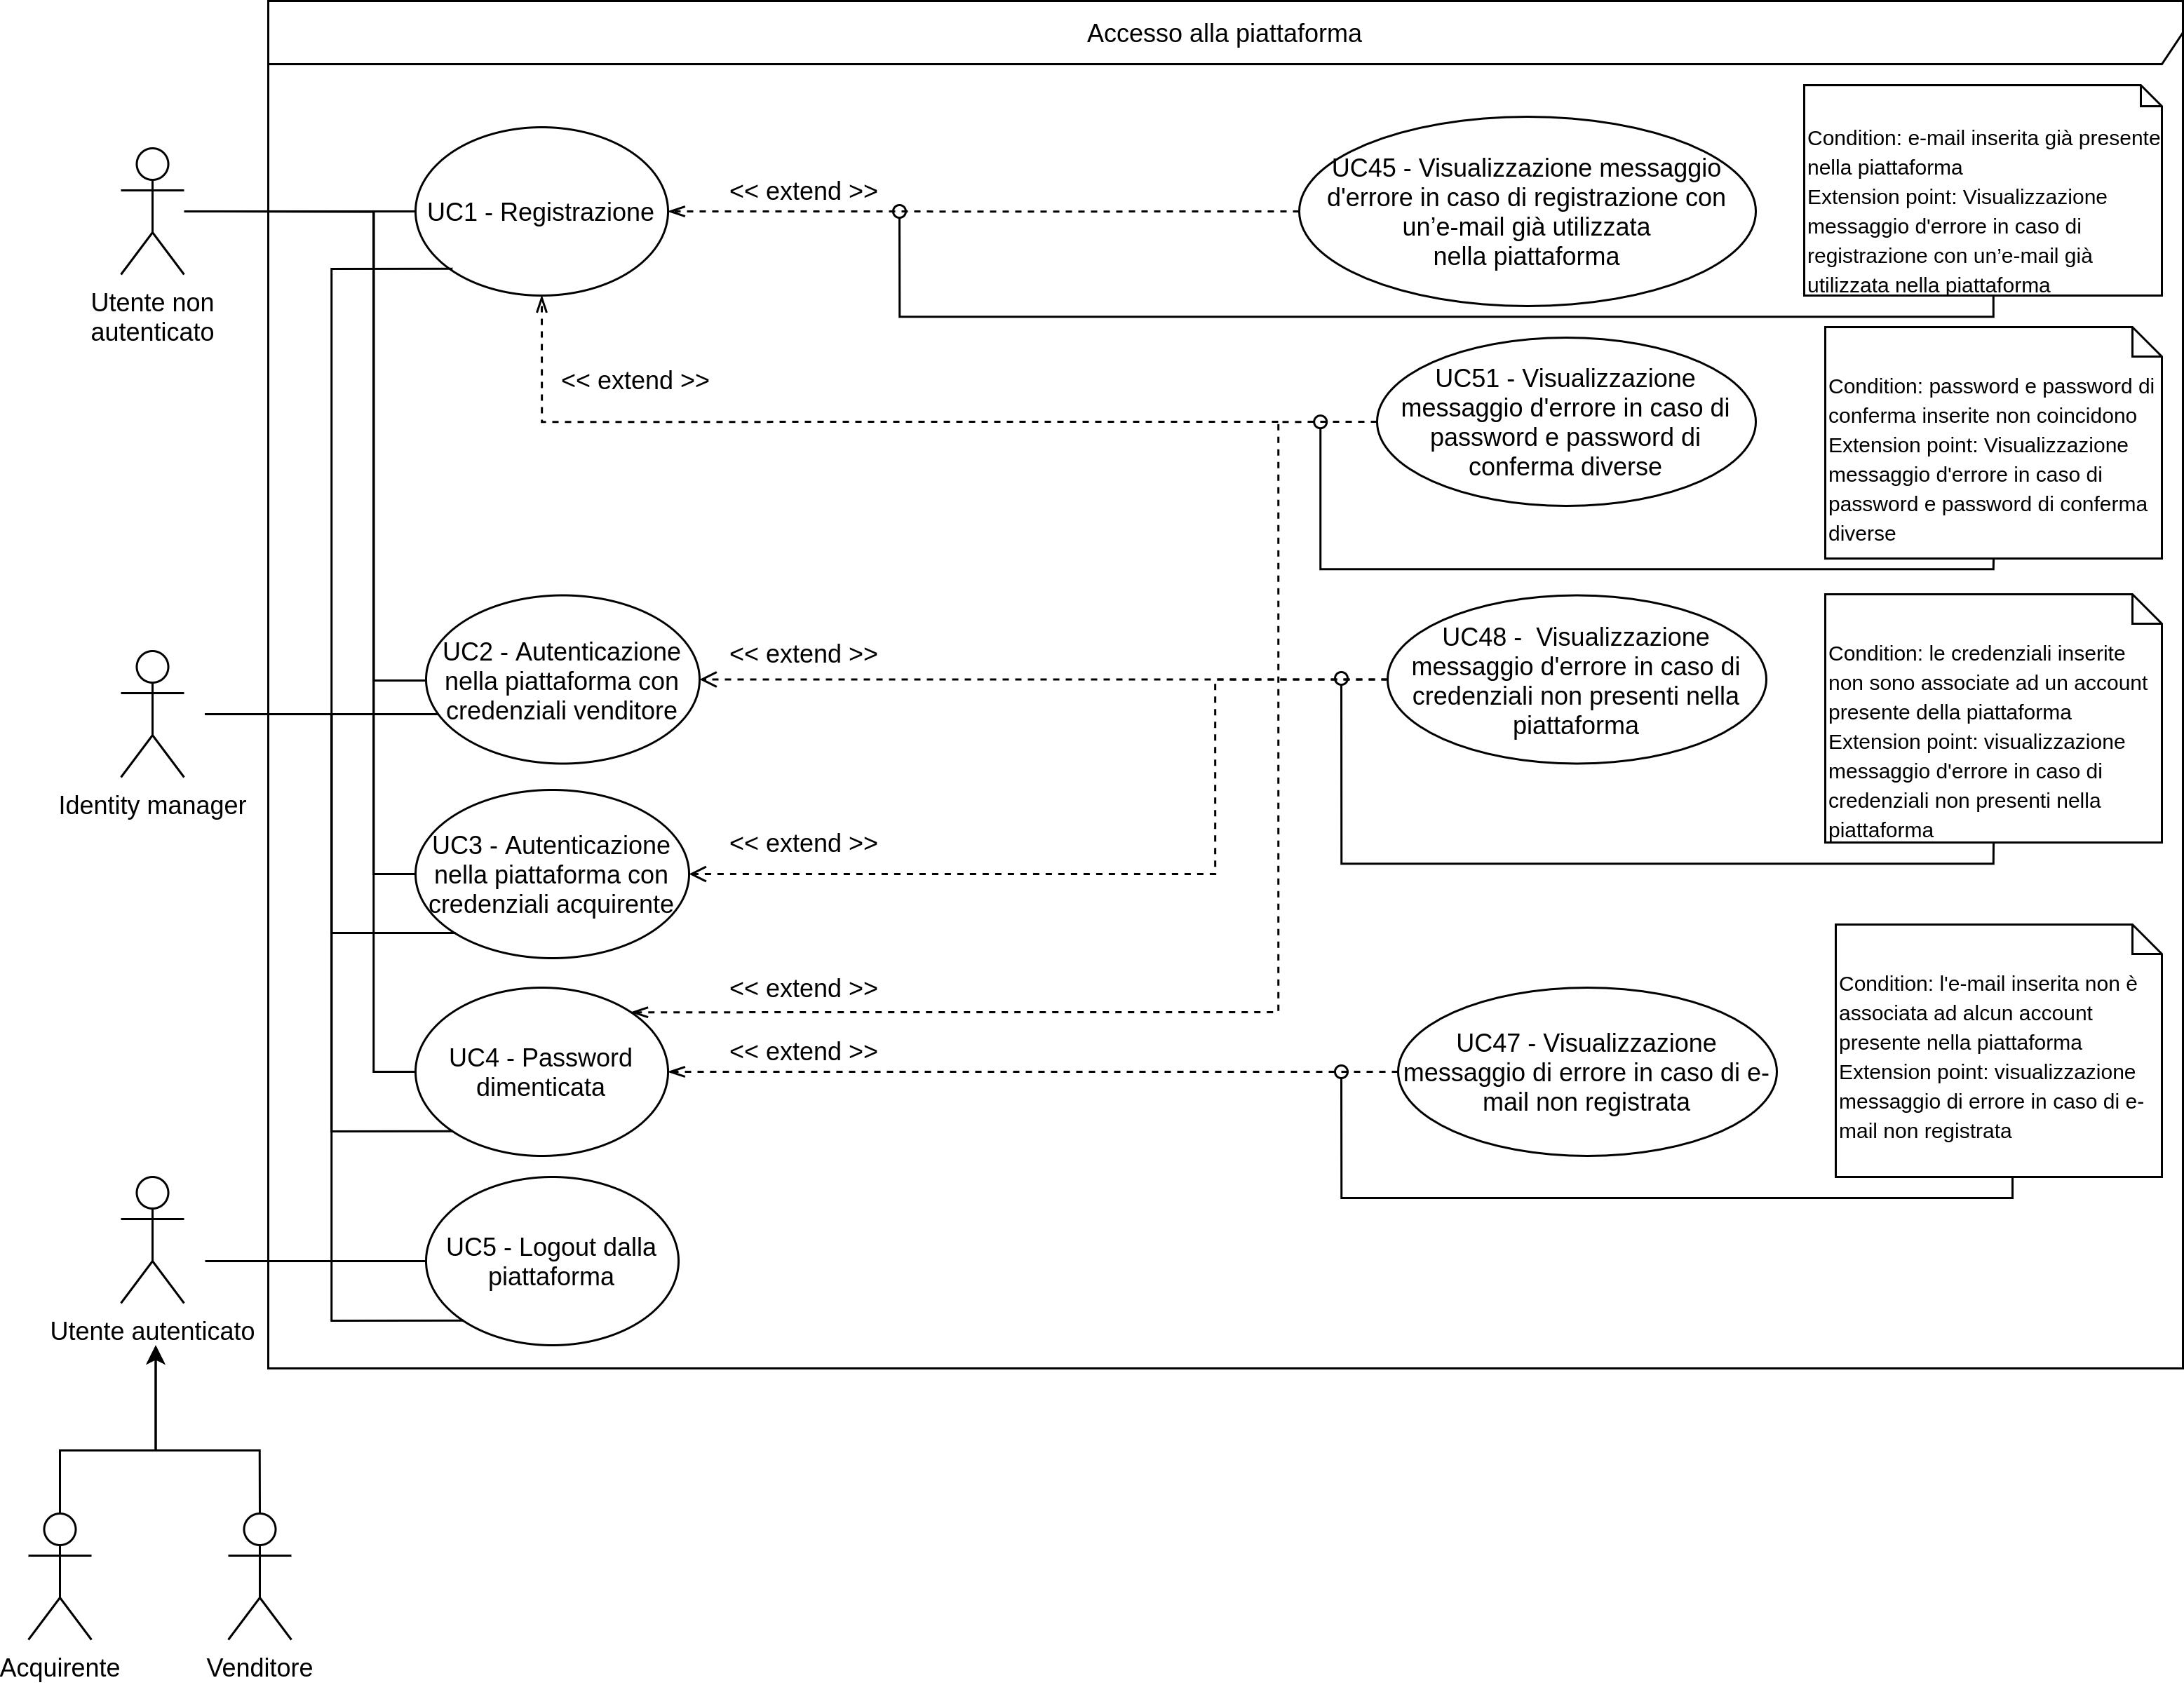
\includegraphics[scale=0.50]{Immagini/DiagrammiUC/AccessoAllaPiattaforma.png}
    \caption{Riepilogo dei casi d'uso di accesso alla piattaforma} 
    \label{fig:riepilogo-accesso-alla-piattaforma}
\end{figure}

\begin{figure}[H]
    \centering
    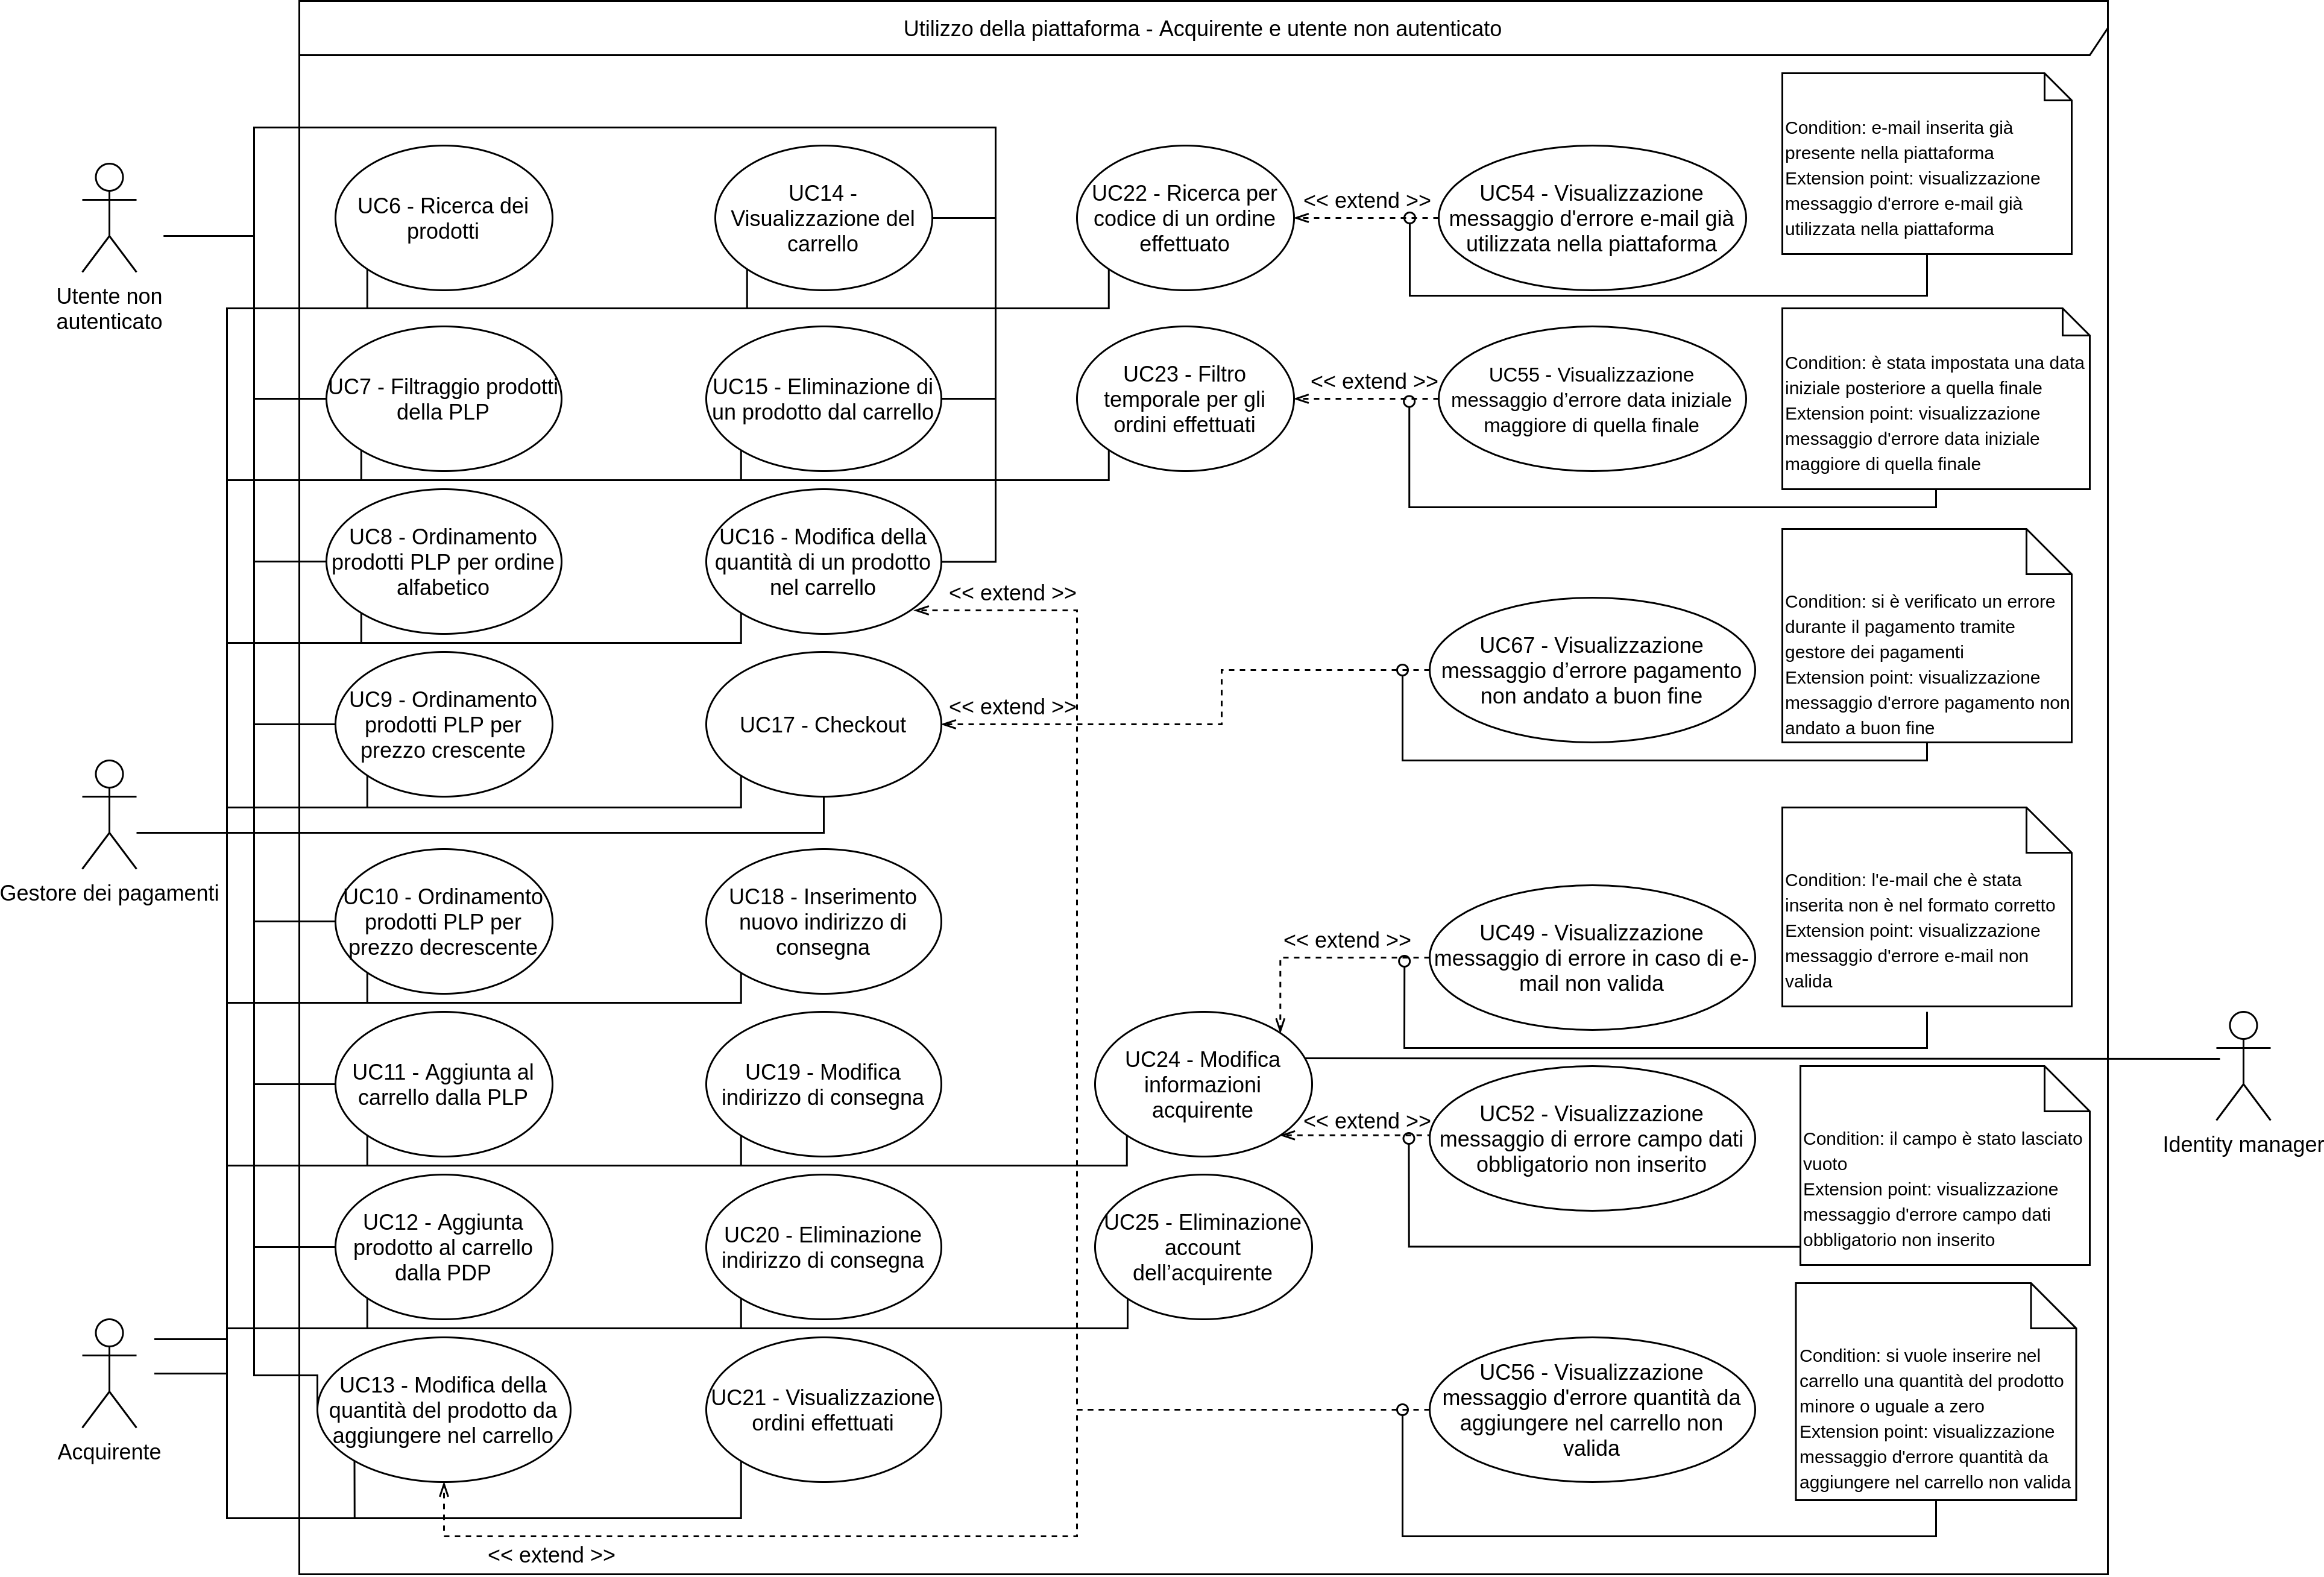
\includegraphics[scale=0.46]{Immagini/DiagrammiUC/UsoPiattaformaAcquirenteUtenteNonAutenticato.png}
    \caption{Riepilogo dei casi d'uso dell'acquirente e dell'utente non autenticato}
    \label{fig:uso-piattaforma-acquirente-utente-non-autenticato}
\end{figure}

\begin{figure}[H]
    \centering
    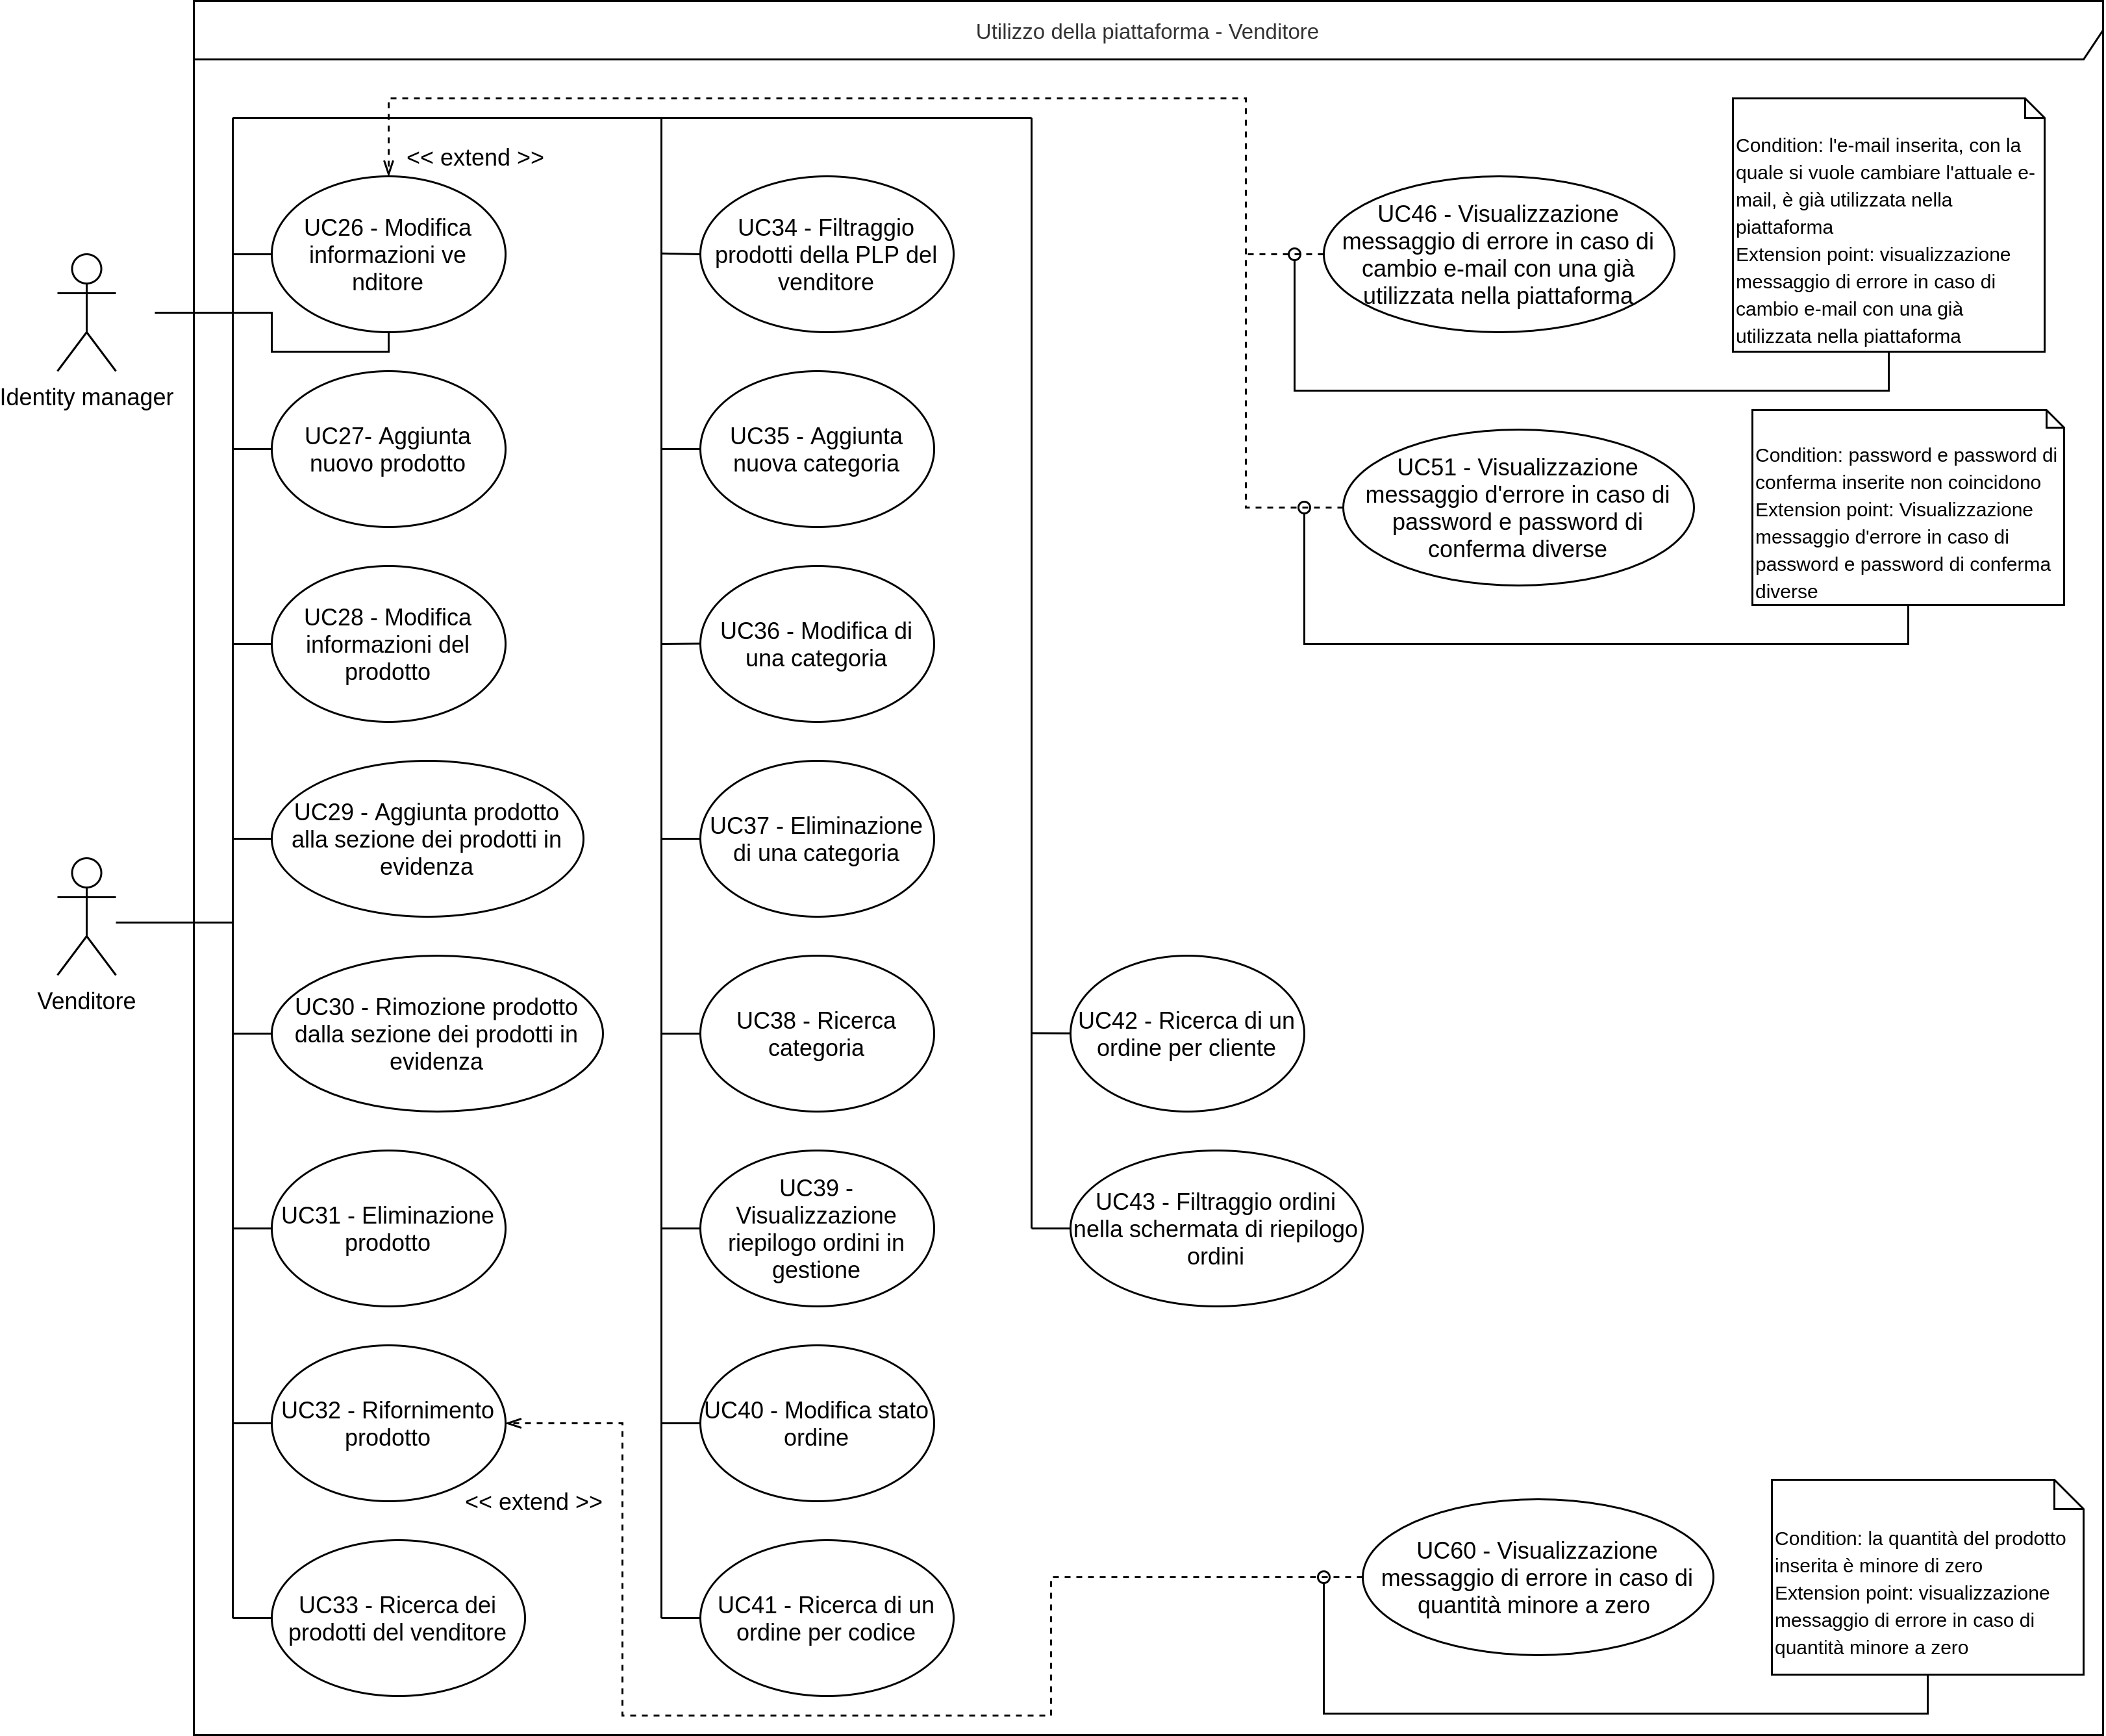
\includegraphics[width=\textwidth]{Immagini/DiagrammiUC/UsoPiattaformaVenditore.png}
    \caption{Riepilogo dei casi d'uso del venditore}
    \label{fig:uso-piattaforma-Venditore}
\end{figure}


\clearpage

% Accesso alla piattaforma
\UC{Registrazione}
\begin{figure}[H]
    \centering
    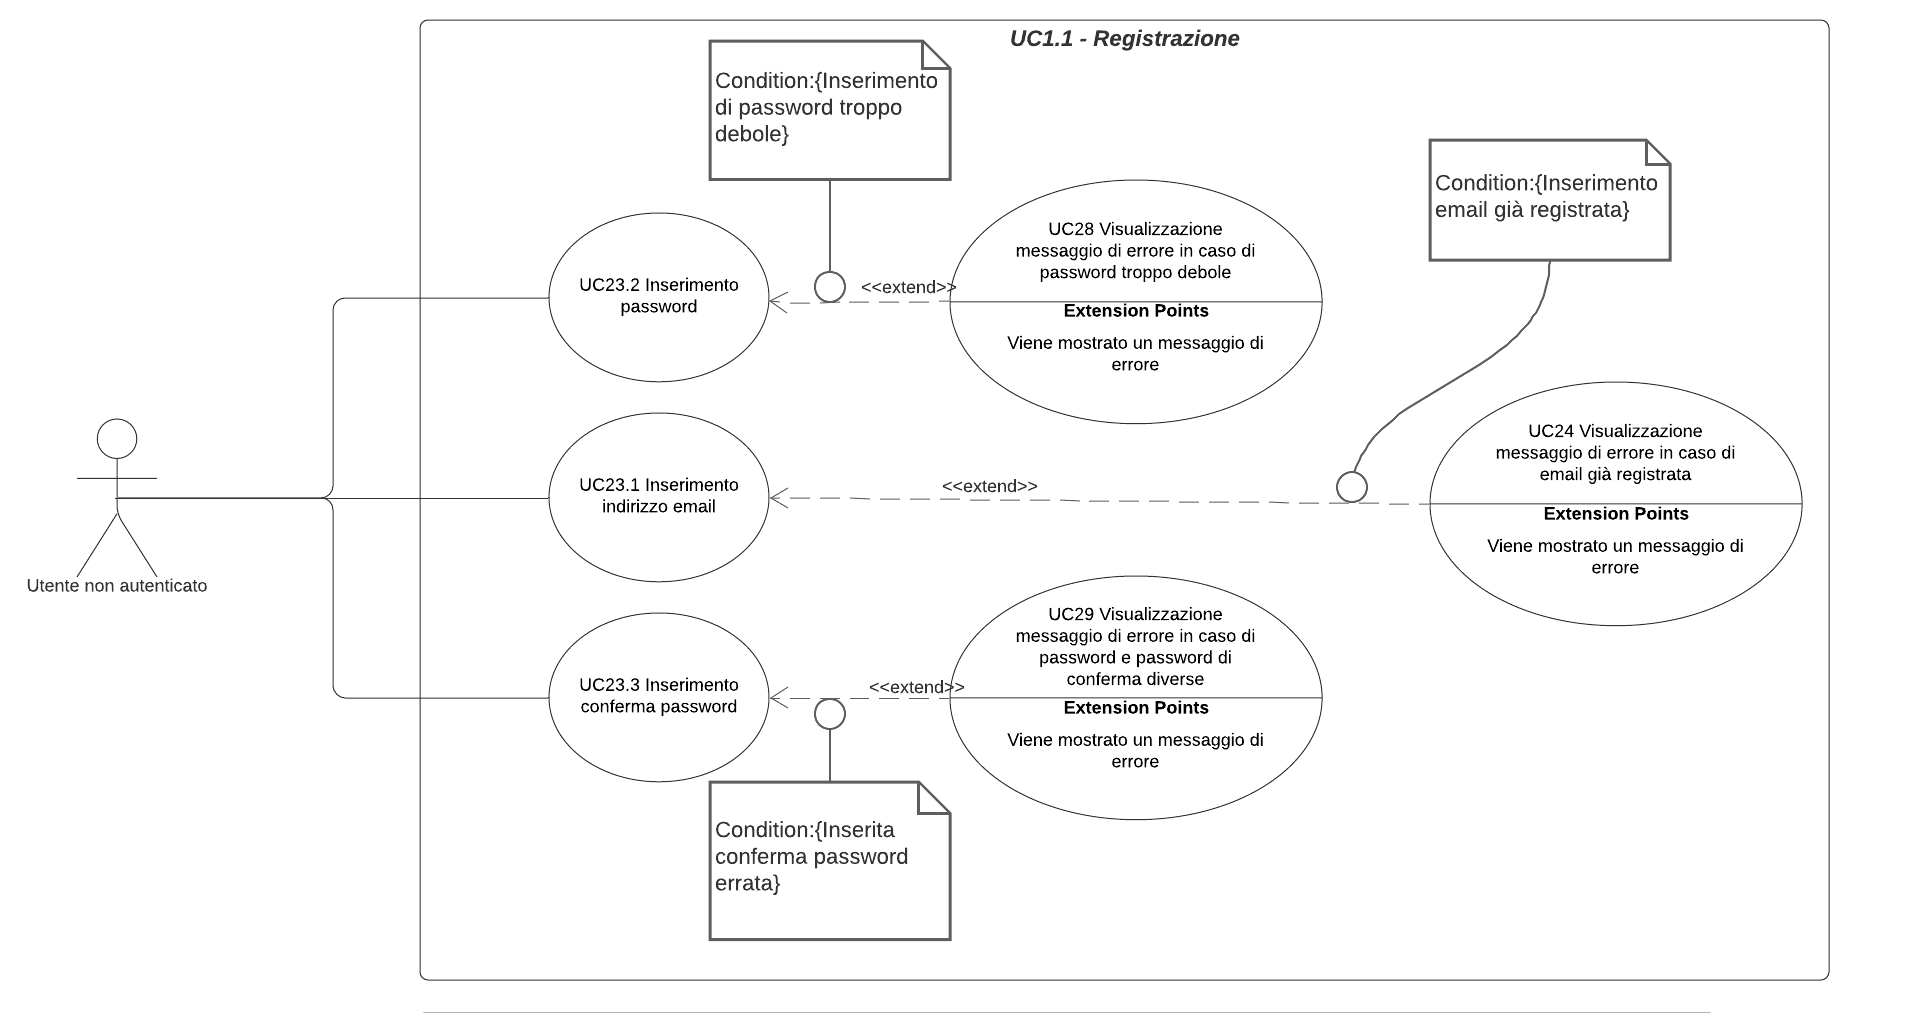
\includegraphics[scale=0.6]{Immagini/DiagrammiUC/UC1.1Registrazione}
    \caption{Diagramma di \actualUC: Registrazione}
    \label{fig:RegistrazionePiattaforma}
\end{figure}

L'utente non autenticato che non dispone di credenziali può registrarsi e accedere come acquirente nella piattaforma usando l'email e la password.
\begin{itemize}
    \item \textbf{Attori primari:} utente non autenticato;
    \item \textbf{Precondizione:} l'utente non è ancora presente nella piattaforma e si trova nella \glo{vista} di registrazione;
    \item \textbf{Postcondizione:} l'utente è registrato con un account acquirente ed è autenticato come tale sulla piattaforma;
    \item \textbf{Scenario principale:} l'utente crea un account compilando tutti i campi del modulo di registrazione nel seguente modo:
    \begin{itemize}
    	\item Inserimento nome;
    	\item Inserimento cognome;
        \item (UC) - Inserimento indirizzo e-mail per la registrazione;
        \item (UC) - Inserimento password per la registrazione;
        \item Inserimento conferma password;
        \item L'utente non autenticato conferma il proprio indirizzo email inserito per la registrazione;
        \item L'utente non autenticato richiede la registrazione.
    \end{itemize}
	\item \textbf{Scenario alternativo:} l'utente inserisce un indirizzo email già presente nella piattaforma
	\begin{itemize}
		\item (UC Estensione) - Viene mostrato un messaggio d'errore;
		\item L'utente non può procedere all'autenticazione.
	\end{itemize}
	\item \textbf{Scenario alternativo:} l'utente non inserisce una o più informazioni obbligatorie
	\begin{itemize}
		\item (UC Estensione) - Viene mostrato un messaggio d'errore;
		\item L'utente non può procedere all'autenticazione.
	\end{itemize}
	\item \textbf{Scenario alternativo:} l'utente compila i campi dati per la password e la conferma della stessa con due password diverse
	\begin{itemize}
		\item (UC Estensione) - Viene mostrato un messaggio d'errore;
		\item L'utente non può procedere all'autenticazione.
	\end{itemize}
	%\item \textbf{Scenario alternativo:} l'utente prova ad eseguire l'operazione di registrazione senza aver compilato alcun campo dati del modulo per eseguire la registrazione;
    \item \textbf{Estensioni:}
    \begin{itemize}
        \item (UC) - Visualizzazione messaggio di errore in caso di email già registrata nella piattaforma;
        \item (UC) - Visualizzazione messaggio di errore in caso di campi dati obbligatori non compilati;
        %\item (UC) - Visualizzazione messaggio di errore in caso di modulo non compilato;
        \item (UC) - Visualizzazione messaggio di errore in caso di password e password di conferma diverse.
    \end{itemize}
	\item \textbf{Inclusioni:}
	\begin{itemize}
		\item (UC) - Inserimento indirizzo email per la registrazione;
		\item (UC) - Inserimento password per la registrazione.
	\end{itemize}
\end{itemize}

\subUC{Inserimento indirizzo email per la registrazione}
L'utente non autenticato inserisce l'indirizzo email.
\begin{itemize}
	\item \textbf{Attori primari:} utente non autenticato;
	\item \textbf{Precondizione:} l'attore non ha ancora fornito un'email e ha a disposizione un campo dati dove inserirla;
	\item \textbf{Postcondizione:} l'utente non autenticato ha fornito un indirizzo email valido;
	\item \textbf{Scenario principale:} l'utente non autenticato inserisce il proprio indirizzo email per procedere con la registrazione;
	\item \textbf{Scenario alternativo:} l'utente non autenticato ha inserito un indirizzo email con un formato non corretto;
	\item \textbf{Estensione:}
	\begin{itemize}
		\item (UC) - Visualizzazione messaggio di errore in caso di email non valida.
	\end{itemize}
\end{itemize}

\subUC{Inserimento password per la registrazione}
L'utente non autenticato inserisce una password.
\begin{itemize}
	\item \textbf{Attori primari:} utente non autenticato;
	\item \textbf{Precondizione:} l'attore non ha ancora fornito una password valida e ha a disposizione un campo dati dove inserirla;
	\item \textbf{Postcondizione:} l'utente ha inserito una password valida.
	\item \textbf{Scenario principale:} l'utente non autenticato inserisce una password che rispetti le condizioni imposte per procedere con la registrazione;
	\item \textbf{Scenario alternativo:} l'utente non autenticato ha inserito una password con un formato non corretto;
	\item \textbf{Estensione:}
	\begin{itemize}
		\item (UC) - Visualizzazione messaggio di errore in caso di password troppo debole.
	\end{itemize}
\end{itemize}

\UC{Autenticazione nella piattaforma con credenziali venditore}
\begin{figure}[H]
    \centering
    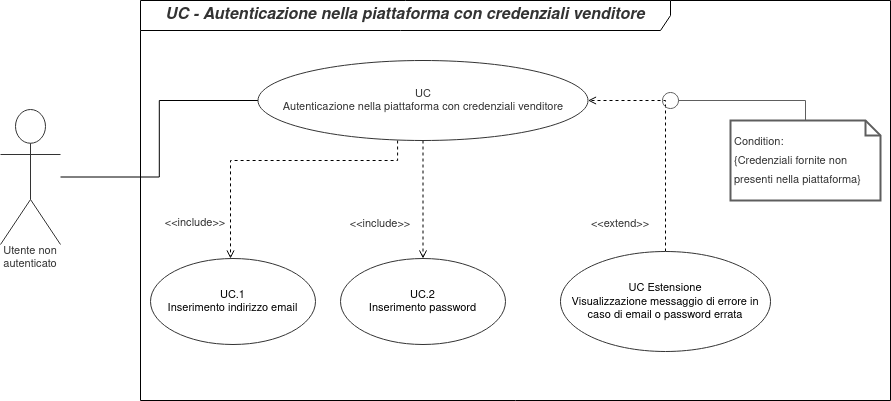
\includegraphics[scale=0.6]{Immagini/DiagrammiUC/AccessoVenditore.png}
    \caption{Diagramma di \actualUC: Autenticazione nella piattaforma con credenziali venditore} 
    \label{fig:LoginVenditore}
\end{figure}

L'utente non autenticato che dispone di credenziali venditore può accedere nella piattaforma usando l'email e la password.
\begin{itemize}
    \item \textbf{Attori primari:} utente non autenticato;
    \item \textbf{Precondizione:} l'utente dispone di credenziali venditore e si trova nella vista di login;
    \item \textbf{Postcondizione:} l'utente è autenticato come venditore e si trova sulla \glo{dashboard};
    \item \textbf{Scenario principale:} l'utente accede alla piattaforma con delle credenziali in questo modo:
    \begin{itemize}
        \item (UC) - Inserimento indirizzo email;
        \item (UC) - Inserimento password;
        \item Richiede l'autenticazione;
        \item L'utente è autenticato come venditore;
        \item L'utente viene portato alla dashboard.
    \end{itemize}
	\item \textbf{Scenario alternativo:} l'utente compila i campi dati con delle credenziali
	\begin{itemize}
		\item Inserimento indirizzo email;
		\item Inserimento password;
        \item Richiede l'autenticazione.
    \end{itemize}
	Ma le credenziali fornite non appartengono alla piattaforma, quindi:
	\begin{itemize}
		\item (UC Estensione) - Viene visualizzato un messaggio di errore apposito;
		\item L'utente rimane non autenticato e alla pagina di login.
	\end{itemize}
    \item \textbf{Estensioni:}
    \begin{itemize}
        \item (UC) - Visualizzazione messaggio di errore in caso di credenziali errate.
    \end{itemize}
    \item \textbf{Inclusioni:}
    \begin{itemize}
    	\item (UC) - Inserimento indirizzo email;
    	\item (UC) - Inserimento password.
    \end{itemize}
\end{itemize}

\resetSubUC
\subUC{Inserimento indirizzo email per l'autenticazione}
\begin{itemize}
	\item \textbf{Attori primari:} utente non autenticato;
	\item \textbf{Precondizione:} l'utente non è autenticato;
	\item \textbf{Postcondizione:} l'utente ha inserito il proprio indirizzo email;
	\item \textbf{Scenario principale:} l'utente non autenticato inserisce l'indirizzo email per l'autenticazione.
	\item \textbf{Scenario alternativo:} l'utente non inserisce l'email:
	\begin{itemize}
		\item (UC) - Viene mostrato un messaggio d'errore;
		\item L'utente non può procedere all'autenticazione.
	\end{itemize}
	\item \textbf{Estensioni:}
	\begin{itemize}
		\item (UC) - Visualizzazione messaggio campo dati obbligatorio non inserito.
	\end{itemize}
\end{itemize}

\subUC{Inserimento password per l'autenticazione}
\begin{itemize}
	\item \textbf{Attori primari:} utente non autenticato;
	\item \textbf{Precondizione:} l'utente non è autenticato;
	\item \textbf{Postcondizione:} l'utente ha inserito la propria password;
	\item \textbf{Scenario principale:} l'utente non autenticato inserisce la password per l'autenticazione;
	\item \textbf{Scenario alternativo:} l'utente non inserisce la password:
	\begin{itemize}
		\item (UC) - Viene mostrato un messaggio d'errore;
		\item L'utente non può procedere all'autenticazione.
	\end{itemize}
	\item \textbf{Estensioni:}
	\begin{itemize}
		\item (UC) - Visualizzazione messaggio campo dati obbligatorio non inserito.
	\end{itemize}
\end{itemize}

\UC{Autenticazione nella piattaforma con credenziali acquirente}
\begin{figure}[H]
	\centering
	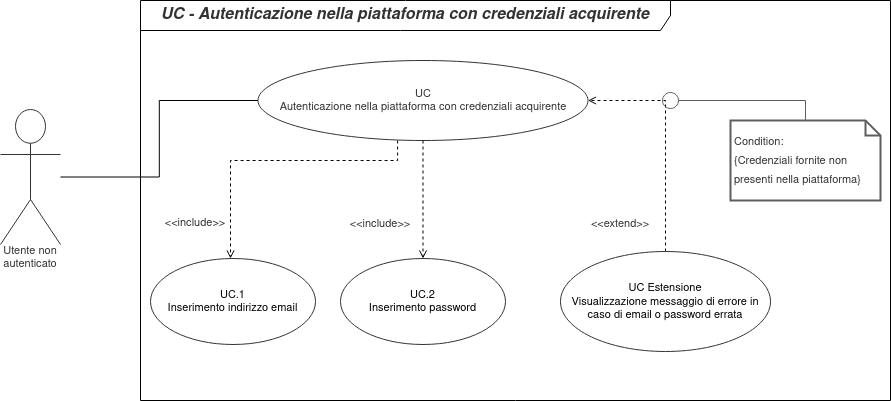
\includegraphics[scale=0.6]{Immagini/DiagrammiUC/AccessoAcquirente.png}
	\caption{Diagramma di \actualUC: Autenticazione nella piattaforma con credenziali acquirente} 
	\label{fig:LoginAcquirente}
\end{figure}

L'utente non autenticato che dispone di credenziali acquirente può accedere nella piattaforma usando l'email e la password.
\begin{itemize}
	\item \textbf{Attori primari:} utente non autenticato;
	\item \textbf{Precondizione:} l'utente dispone di credenziali acquirente e si trova nella vista di login;
	\item \textbf{Postcondizione:} l'utente è autenticato come acquirente e si trova nella vista principale;
	\item \textbf{Scenario principale:} l'utente accede alla piattaforma con delle credenziali in questo modo:
	\begin{itemize}
		\item (UC) - Inserimento indirizzo email venditore;
		\item (UC) - Inserimento password;
		\item Richiede l'autenticazione;
		\item L'utente è autenticato come acquirente;
		\item L'utente viene portato alla vista principale.
	\end{itemize}
	\item \textbf{Scenario alternativo:} l'utente compila i campi dati con delle credenziali
	\begin{itemize}
		\item (UC) - Inserimento indirizzo;
		\item (UC) - Inserimento password;
		\item Richiede l'autenticazione.
	\end{itemize}
	Ma le credenziali fornite non appartengono alla piattaforma, quindi:
	\begin{itemize}
		\item (UC Estensione) - Viene visualizzato un messaggio di errore apposito;
		\item L'utente rimane non autenticato e alla pagina di login.
	\end{itemize}
	\item \textbf{Estensioni:}
	\begin{itemize}
		\item (UC) - Visualizzazione messaggio di errore in caso di credenziali errate.
	\end{itemize}
	\item \textbf{Inclusioni:}
	\begin{itemize}
		\item (UC) - Inserimento indirizzo email;
		\item (UC) - Inserimento  password. 
		\end{itemize}
\end{itemize}

\UC{Password dimenticata}
\begin{figure}[H]
    \centering
    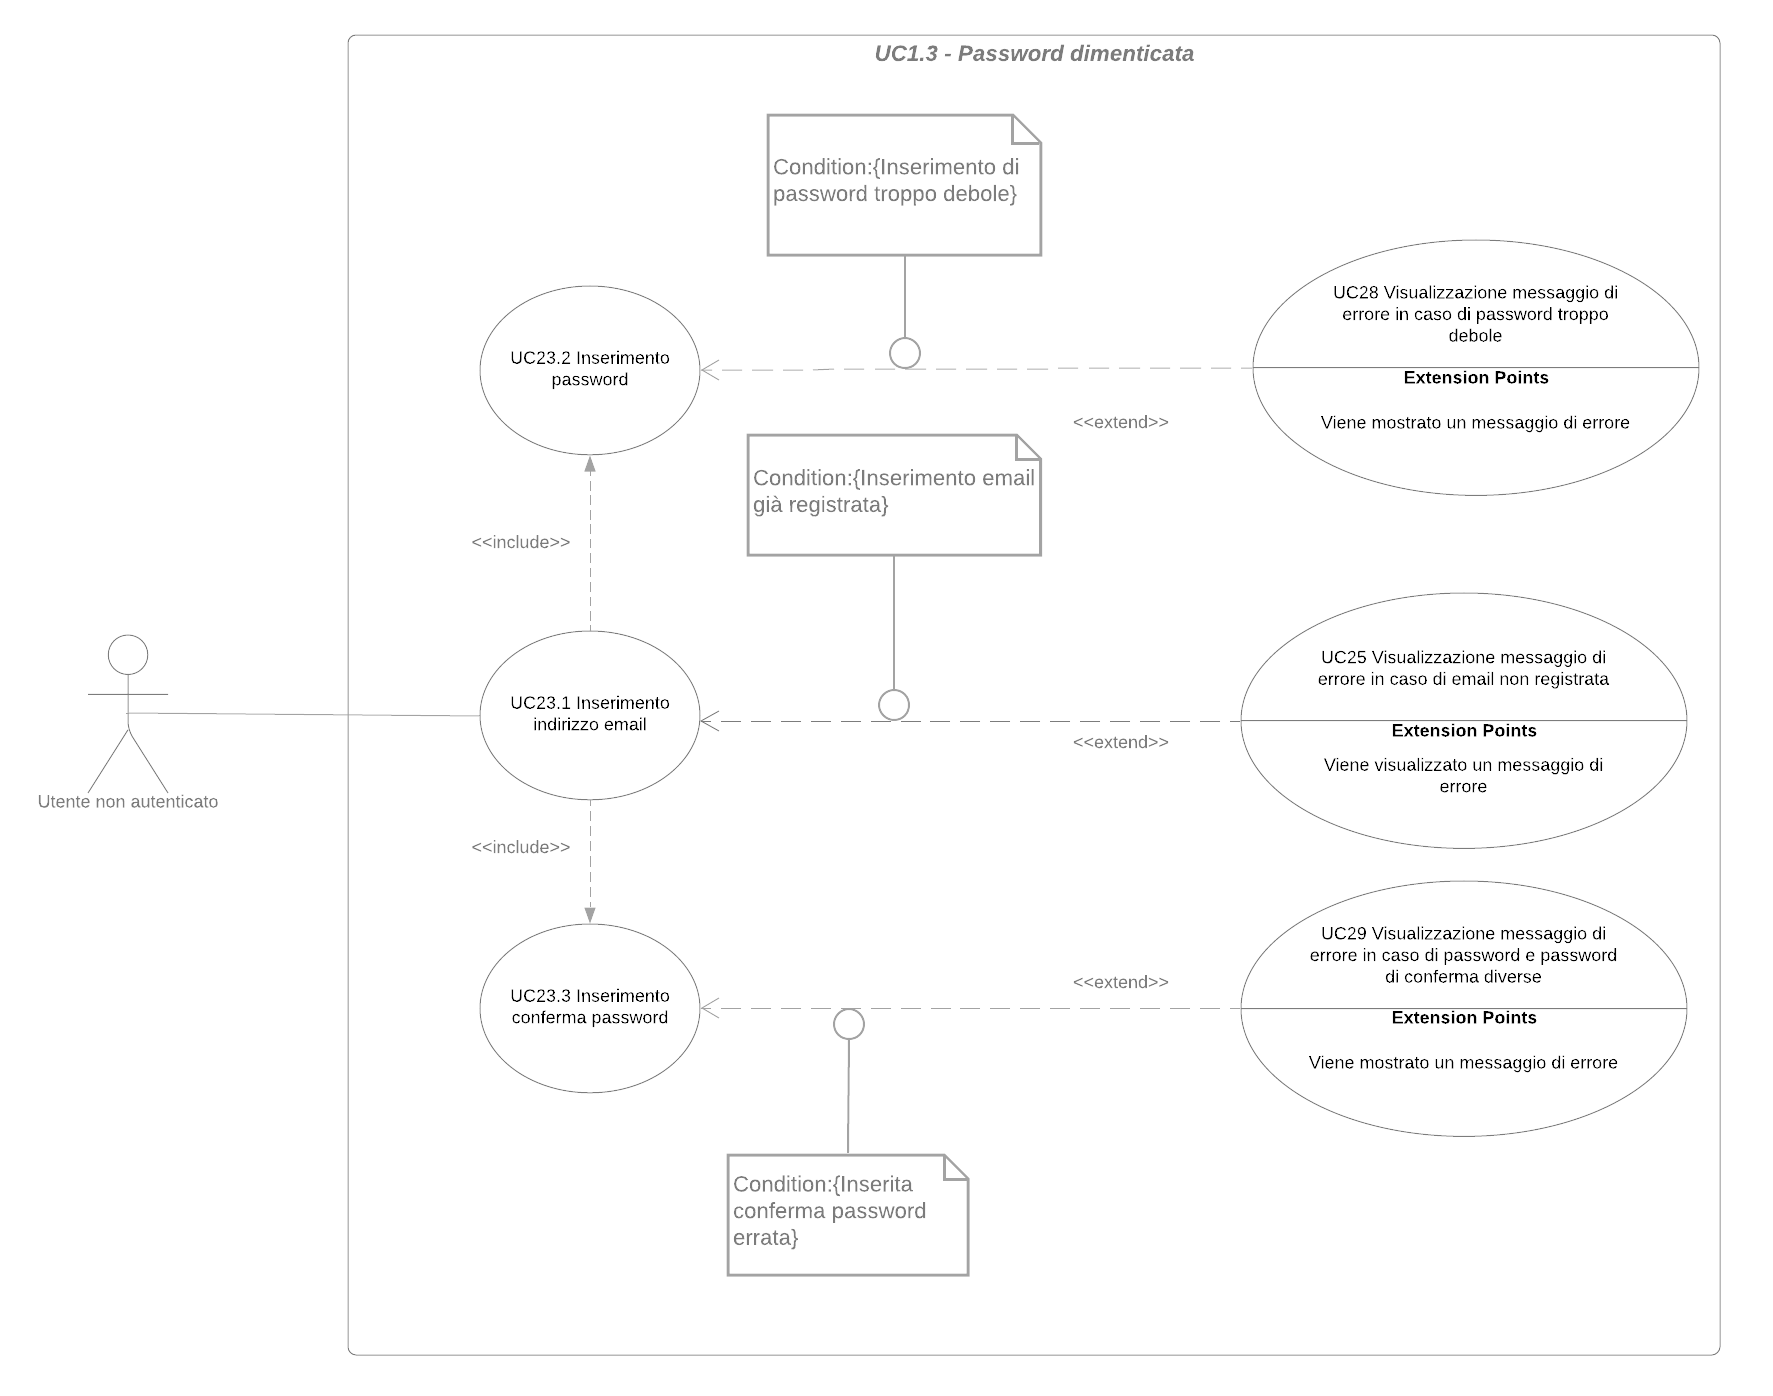
\includegraphics[scale=0.2]{Immagini/DiagrammiUC/UC1.3PasswordDimenticata.png}
    \caption{Diagramma di \actualUC: Password dimenticata} 
    \label{fig:PasswordDimenticata}
\end{figure}

L'utente che dispone di credenziali si è dimenticato la propria password e la vuole cambiare.
\begin{itemize}
    \item \textbf{Attori primari:} utente non autenticato;
    \item \textbf{Precondizione:} l'utente non autenticato che dispone di credenziali si trova nella vista per cambiare la password;
    \item \textbf{Postcondizione:} l'utente è autenticato e ha cambiato la password con cui poter effettuare l'accesso alla piattaforma;
    \item \textbf{Scenario principale:} l'utente che dispone di credenziali si è dimenticato la propria password e per cambiarla deve compiere i seguenti passi:
    \begin{itemize}
        \item (UC) - Inserimento indirizzo email;
        \item Invio link per il cambio della password all'indirizzo email indicato;
        \item Apertura della vista per il cambio della password;
        \item (UC) - Inserimento nuova password;
        \item Inserimento conferma nuova password;
        \item L'utente è autenticato e ha cambiato la password.
    \end{itemize}
	\item \textbf{Scenario alternativo:} l'utente compila i campi dati
	\begin{itemize}
		\item (UC) - Inserimento indirizzo email.
	\end{itemize}
	Ma l'indirizzo email non appartiene alla piattaforma, quindi:
	\begin{itemize}
		\item (UC Estensione) - Viene visualizzato un messaggio di errore apposito;
		\item L'utente rimane non autenticato e alla vista di login.
	\end{itemize}
	\item \textbf{Scenario alternativo:} l'utente compila i campi dati
	\begin{itemize}
		\item (UC) - Inserimento indirizzo email;
		\item Invio link per il cambio della password all'indirizzo email indicato;
		\item Apertura della vista per il cambio della password;
		\item (UC Estensione) - Inserimento nuova password;
		\item Inserimento conferma nuova password;
	\end{itemize}
	Ma la password inserita non è valida, quindi:
	\begin{itemize}
		\item (UC Estensione) - Viene visualizzato un messaggio di errore apposito;
		\item L'utente rimane non autenticato e alla vista di login. 
	\end{itemize}
    \item \textbf{Estensioni:}
    \begin{itemize}
        \item (UC) - Visualizzazione messaggio di errore in caso di email non registrata;
        \item (UC) - Visualizzazione messaggio di errore in caso di password e password di conferma diverse.
    \end{itemize}
    \item \textbf{Inclusioni:}
    \begin{itemize}
        \item (UC) - Inserimento nuova password.
    \end{itemize}
\end{itemize}

\UC{Logout dalla piattaforma}
L'utente autenticato decide di scollegarsi dalla piattaforma.
\begin{itemize}
    \item \textbf{Attori primari:} utente autenticato;
    \item \textbf{Precondizione:} l'utente ha eseguito il login precedentemente e vuole scollegarsi dalla piattaforma;
    \item \textbf{Postcondizione:} l'utente autenticato diventa un utente non autenticato;
    \item \textbf{Scenario principale:} l'utente autenticato decide di scollegarsi dalla piattaforma e compie l'azione di scollegamento.
\end{itemize}

% Ricerca dei prodotti
\UC{Ricerca dei prodotti} 
L'utente non autenticato o l'acquirente può ricercare i prodotti dalla schermata principale oppure dalla PLP.
\begin{itemize}
    \item \textbf{Attori primari:} acquirente o utente non autenticato;
    \item \textbf{Precondizione:} l'attore ha selezionato l'azione della ricerca e inserito le parole per la ricerca del prodotto;
    \item \textbf{Postcondizione:} l'attore viene spostato alla PLP con i prodotti che contengono almeno una delle parole ricercate nella descrizione o nel nome;
    \item \textbf{Scenario principale:} 
    \begin{itemize}
        \item l'attore inserisce le parole per la ricerca del prodotto;
        \item preme sull'azione di ricerca;
        \item viene portato alla PLP che contiene tutti i prodotti che hanno almeno una delle parole indicate nella descrizione o il titolo
    \end{itemize}
    \item \textbf{Estensioni:}
    \begin{enumerate}
        \item l'attore ha svolto una ricerca che non ha prodotto alcun risultato. In questo caso:
        \begin{itemize}
            \item (UC) - viene visualizzato il messaggio di ricerca o filtraggio senza alcun risultato.
        \end{itemize}
    \end{enumerate}
\end{itemize}

\UC{Filtraggio prodotti della PLP}
\begin{figure}[H]
    \centering
    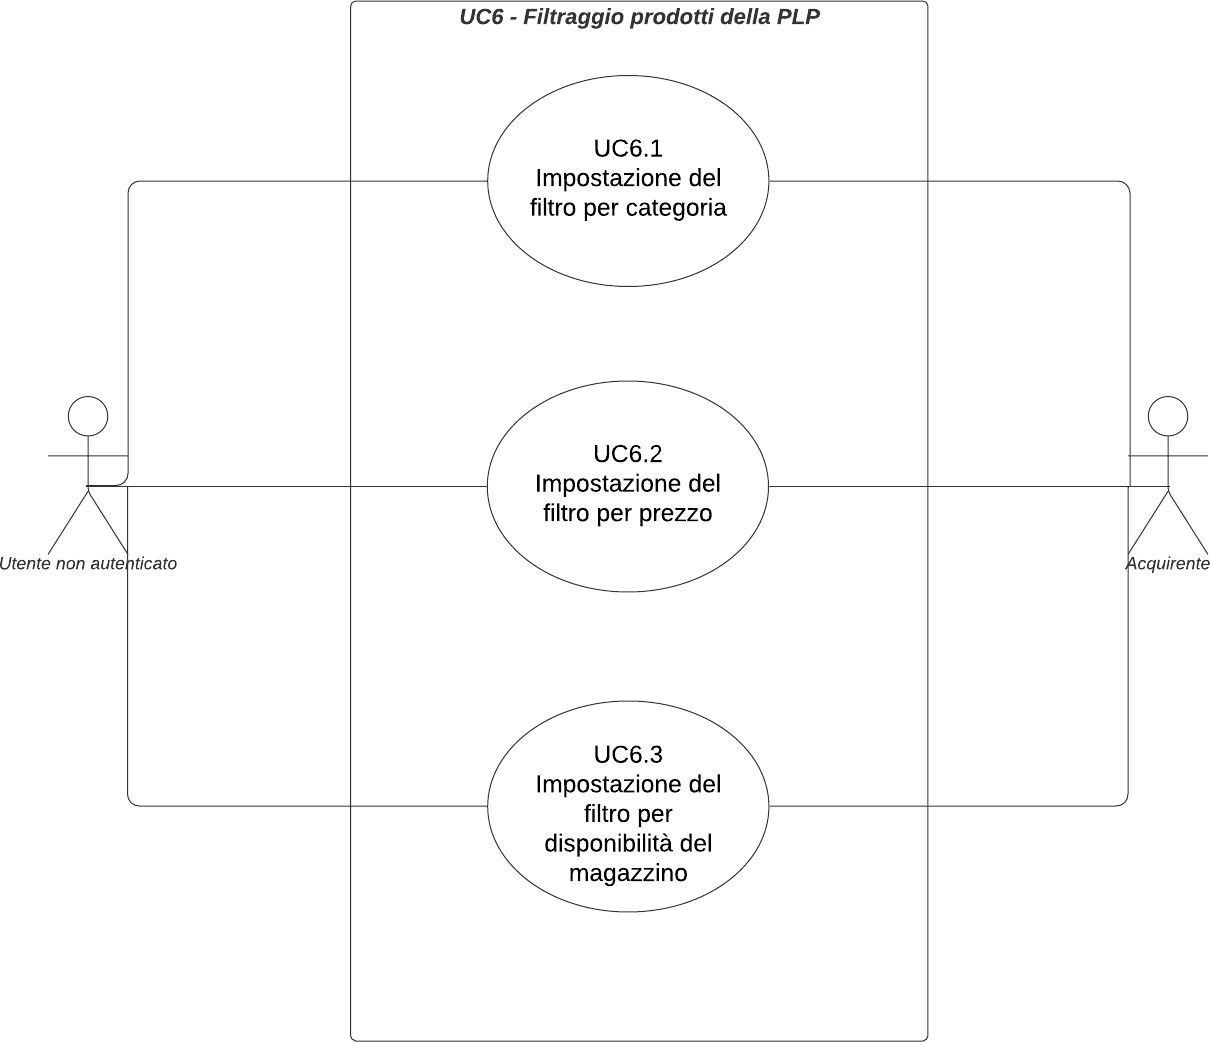
\includegraphics[scale=0.5]{Immagini/DiagrammiUC/UC6FiltraggioProdottiDellaPLP.png}
    \caption{Diagramma di \actualUC: Filtraggio dei prodotti della PLP} 
\end{figure}

L'utente non autenticato o l'acquirente filtra i prodotti all'interno della PLP in base alla categoria, per prezzo, per promozioni attive, sconti applicati e se c'è disponibilità nel magazzino.
\begin{itemize}
    \item \textbf{Attori Primari:} Acquirente; Utente non autenticato.
    \item \textbf{Precondizione:} L'attore è nella PLP e ha impostato uno (o più) dei filtri disponibili per i quali cercare.
    \item \textbf{Postcondizione:} L'attore avrà a disposizione tutti i prodotti che soddisfano tutte le condizioni dei vari filtri impostati.
    \item \textbf{Scenario Principale:}
    \begin{itemize}
        \item l'attore imposta uno (o più) dei filtri seguenti 
        \begin{itemize}
            \item (\actualUC.1) - impostazione del filtro per categoria;
            \item (\actualUC.2) - impostazione del filtro per prezzo;
            \item (\actualUC.3) - impostazione del filtro per disponibilità nel magazzino.
        \end{itemize}
        \item la pagina viene aggiornata con i prodotti che rispettano i filtri applicati;
    \end{itemize}
    \item \textbf{Estensioni:}
    \begin{enumerate}
        \item l'attore ha impostato i seguenti filtri in modo tale che la combinazione con la ricerca non dia alcun risultato. In questo caso:
        \begin{itemize}
            \item (UC) - viene visualizzato il messaggio di ricerca senza alcun risultato.
        \end{itemize}
    \end{enumerate}
\end{itemize}

\resetSubUC

\subUC{Filtro per categorie}
L'utente non autenticato o l'acquirente può cercare i prodotti in base alla loro categoria, selezionando tra tutte le categorie disponibili.
\begin{itemize}
    \item \textbf{Attori Primari:} acquirente o utente non autenticato;
    \item \textbf{Precondizione:} l'attore è nella PLP e ha selezionato una (o più) categorie di quelle disponibili per quale filtrare;
    \item \textbf{Postcondizione:} l'attore avrà a disposizione i prodotti filtrati in base alle categorie selezionate;
    \item \textbf{Scenario principale:} l'attore seleziona le categorie per filtrare i prodotti.
\end{itemize}

\subUC{Filtro per prezzo}
L'utente non autenticato o l'acquirente può cercare i prodotti in base al loro prezzo.
\begin{itemize}
    \item \textbf{Attori Primari:} Acquirente; Utente non autenticato.
    \item \textbf{Precondizione:} L'attore è nella PLP e ha selezionato uno tra gli intervalli di prezzo disponibili (0 - 20, 20 - 50, 50 - 100, 100 - 200, 200 - 500, più di 500), oppure inserito un intervallo personalizzato.
    \item \textbf{Postcondizione:} L'attore avrà a disposizione i prodotti filtrati in base all'intervallo di prezzo selezionato.
    \item \textbf{Scenario Principale:} L'attore seleziona l'intervallo di prezzo oppure ne fornisce uno personalizzato per filtrare i prodotti.
\end{itemize}

\subUC{Filtro per disponibilità nel magazzino}
L'utente non autenticato o l'acquirente può cercare i prodotti in base alla loro disponibilità in magazzino.
\begin{itemize}
    \item \textbf{Attori Primari:} Acquirente; Utente non autenticato.
    \item \textbf{Precondizione:} L'attore è nella PLP e ha attivato il filtro per disponibilità in magazzino.
    \item \textbf{Postcondizione:} L'attore avrà a disposizione i prodotti che sono disponibili in magazzino.
    \item \textbf{Scenario Principale:} L'attore vuole visualizzare tutti i prodotti che sono disponibili in magazzino.
\end{itemize}

 
% Product list page
%%%%%%%%%%%%%%%%%%%%%%%%%%%%%%%%%%%%%%%%%%%%%%%%%%%%%%%%%%%%%%%%%%%%%%%%%%%%%%%%%%%%%%%%%%%%%%%%%%%%%%%%%%%%%%%%%

\UC{Ordinamento prodotti PLP per ordine alfabetico}
\label{ordinamento-alfabetico}

L'utente non autenticato o l'acquirente può ordinare i prodotti risultanti dalla ricerca effettuata in precedenza per ordine alfabetico.
\begin{itemize}
    \item \textbf{Attori primari:} acquirente o utente non autenticato;
    \item \textbf{Precondizione:} l'attore è nella PLP e ha selezionato l'ordinamento per ordine alfabetico;
    \item \textbf{Postcondizione:} i prodotti nella schermata vengono ordinati in ordine alfabetico;
    \item \textbf{Scenario principale:} l'attore vuole ordinare i prodotti nella schermata così da averli elencati in ordine alfabetico.
\end{itemize}

%%%%%%%%%%%%%%%%%%%%%%%%%%%%%%%%%%%%%%%%%%%%%%%%%%%%%%%%%%%%%%%%%%%%%%%%%%%%%%%%%%%%%%%%%%%%%%%%%%%%%%%%%%%%%%%%%

\UC{Ordinamento prodotti PLP per prezzo crescente}
\label{ordinamento-prezzo-crescente}

L'utente non autenticato o l'acquirente può ordinare i prodotti risultanti dalla ricerca effettuata in precedenza per prezzo crescente.
\begin{itemize}
    \item \textbf{Attori primari:} acquirente o utente non autenticato;
    \item \textbf{Precondizione:} l'attore è nella PLP e ha selezionato l'ordinamento per prezzo crescente;
    \item \textbf{Postcondizione:} i prodotti nella schermata vengono ordinati in ordine di prezzo crescente;
    \item \textbf{Scenario principale:} l'attore vuole ordinare i prodotti nella schermata così da averli elencati dal più economico al più costoso.
\end{itemize}

%%%%%%%%%%%%%%%%%%%%%%%%%%%%%%%%%%%%%%%%%%%%%%%%%%%%%%%%%%%%%%%%%%%%%%%%%%%%%%%%%%%%%%%%%%%%%%%%%%%%%%%%%%%%%%%%%

\UC{Ordinamento prodotti PLP per prezzo decrescente}
\label{ordinamento-prezzo-decrescente}

L'utente non autenticato o l'acquirente può ordinare i prodotti risultanti dalla ricerca effettuata in precedenza per prezzo decrescente.
\begin{itemize}
    \item \textbf{Attori primari:} acquirente o utente non autenticato;
    \item \textbf{Precondizione:} l'attore è nella PLP e ha selezionato l'ordinamento per prezzo decrescente;
    \item \textbf{Postcondizione:} i prodotti nella schermata vengono ordinati in ordine di prezzo decrescente;
    \item \textbf{Scenario principale:} l'attore vuole ordinare i prodotti nella schermata così da averli elencati dal più costoso al più economico.
\end{itemize}

%%%%%%%%%%%%%%%%%%%%%%%%%%%%%%%%%%%%%%%%%%%%%%%%%%%%%%%%%%%%%%%%%%%%%%%%%%%%%%%%%%%%%%%%%%%%%%%%%%%%%%%%%%%%%%%%%

\UC{Aggiunta al carrello dalla PLP}
\label{aggiunta-carrello-plp}

\begin{figure}[H]
    \centering
    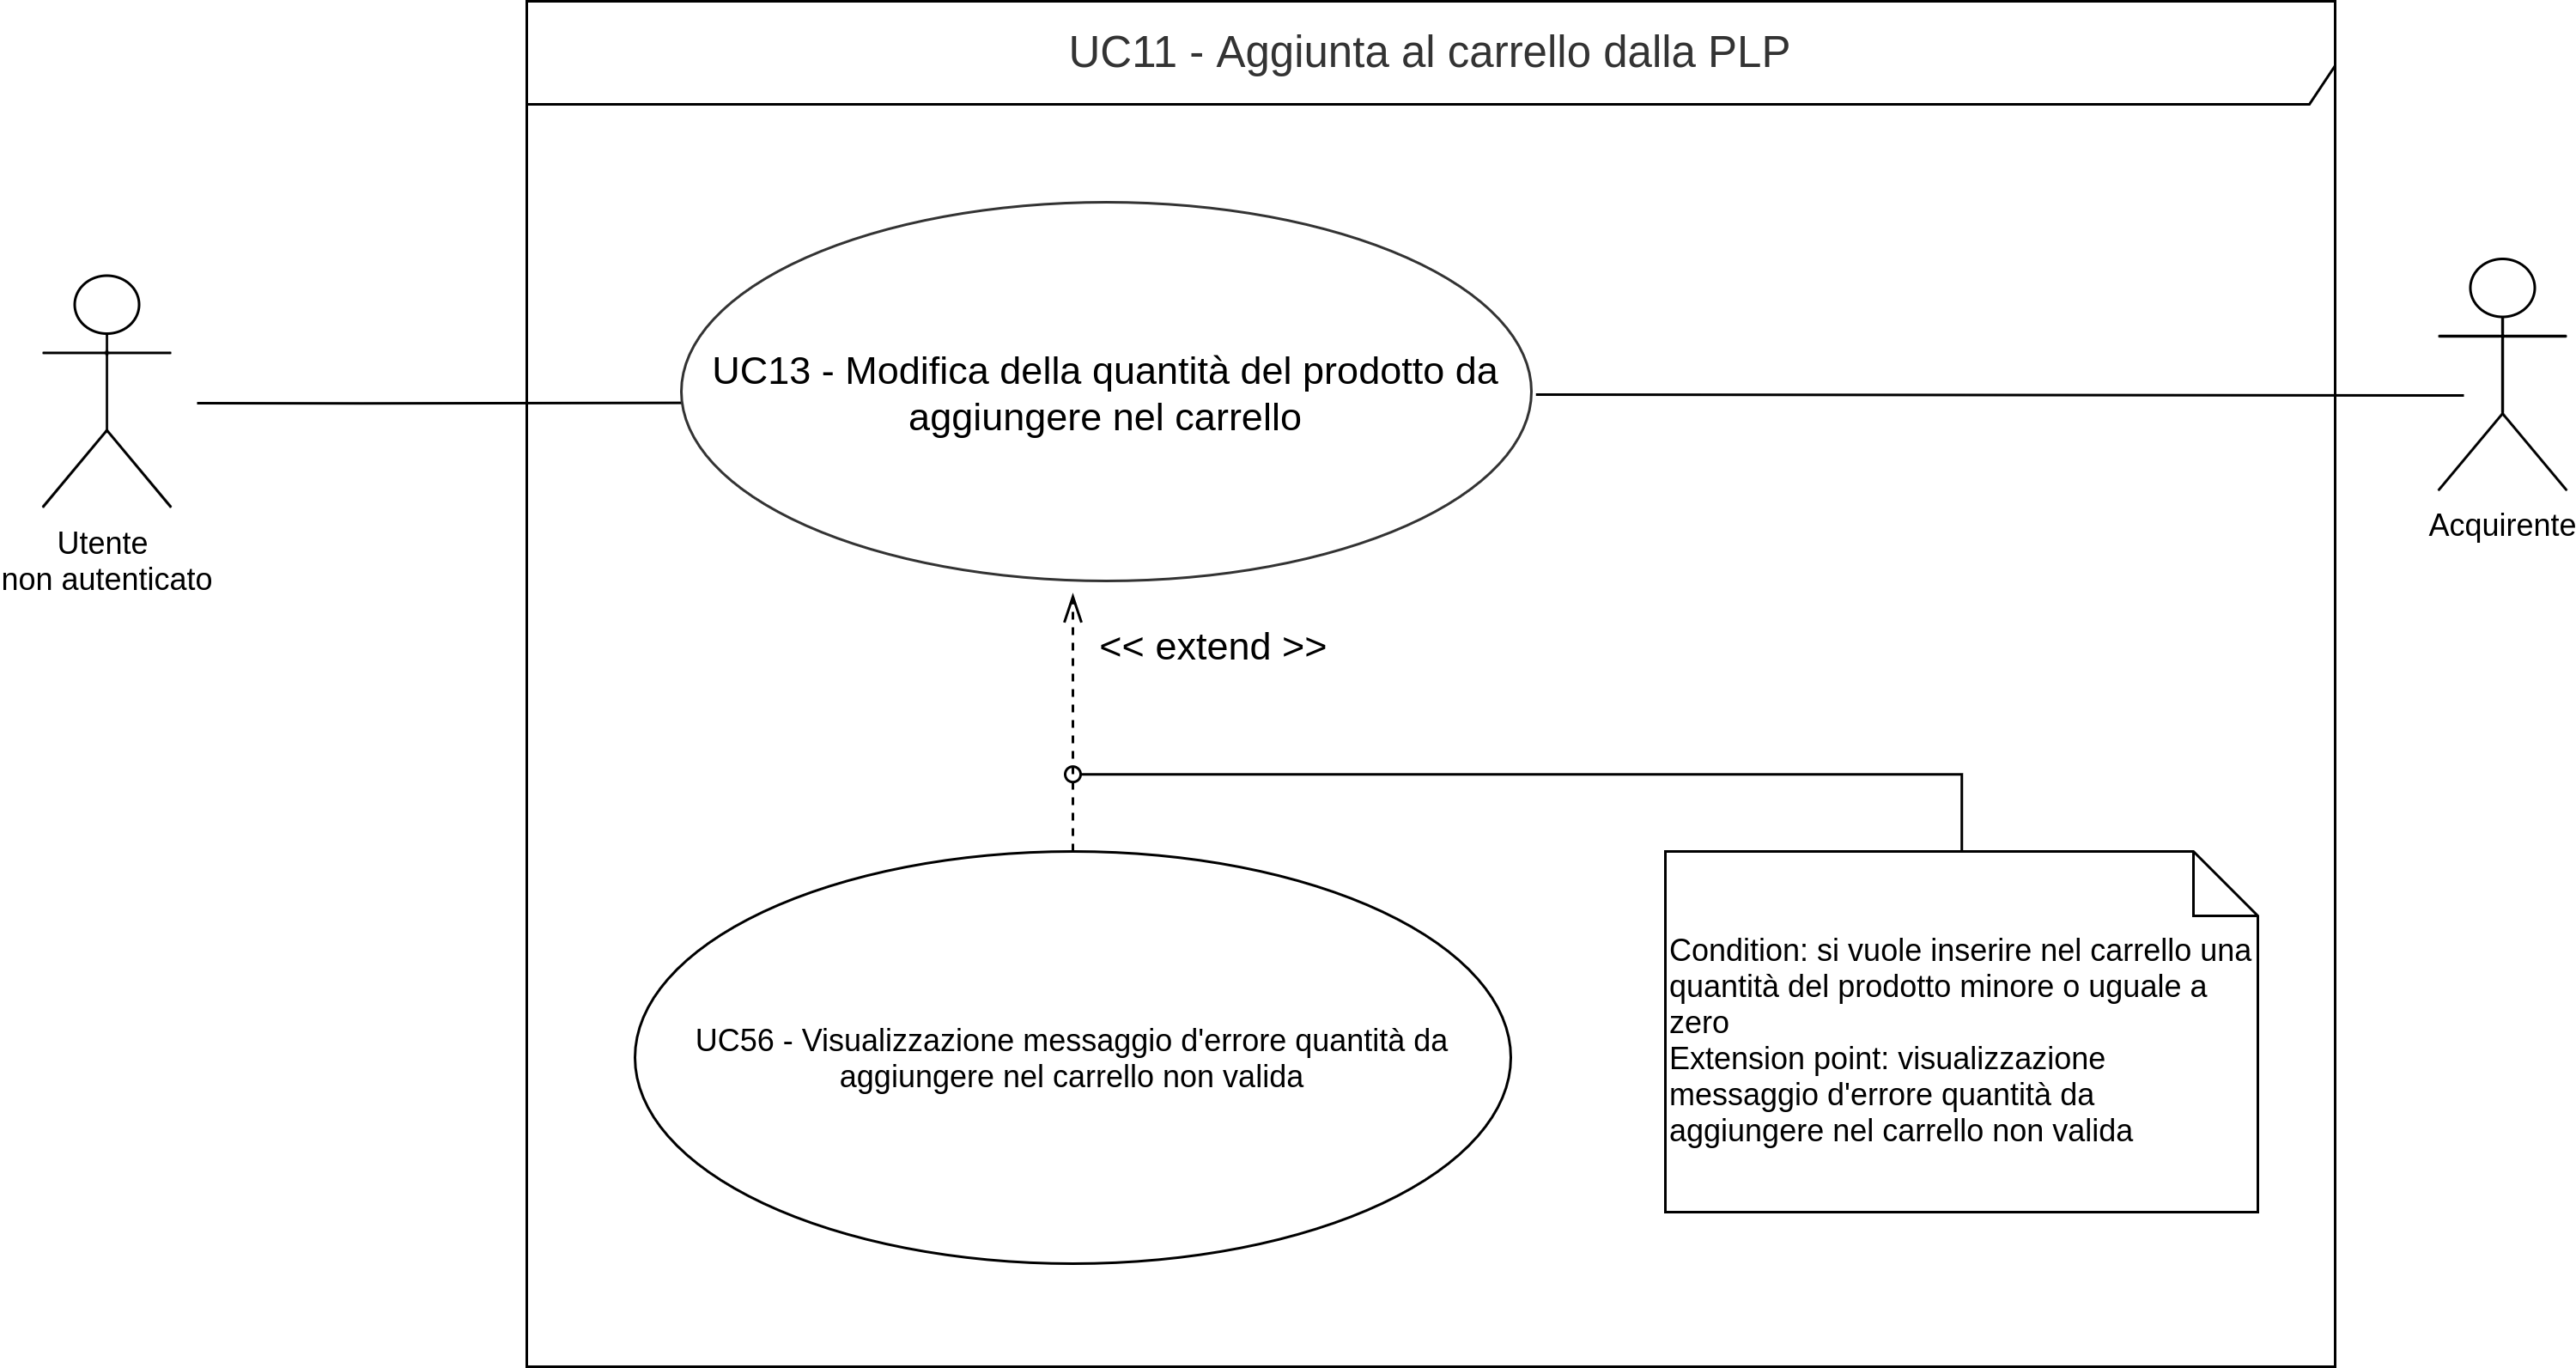
\includegraphics[scale=0.6]{Immagini/DiagrammiUC/AggiuntaProdottiCarrelloPLP.png}
    \caption{Diagramma di \actualUC: Aggiunta al carrello dalla PLP}
\end{figure}

L'utente non autenticato o l'acquirente può aggiungere al carrello i prodotti direttamente dalla PLP.
\begin{itemize}
    \item \textbf{Attori primari:} acquirente o utente non autenticato;
    \item \textbf{Precondizione:} l'attore si trova nella PLP;
    \item \textbf{Postcondizione:} l'attore rimane nella PLP ed al carrello è stato aggiunto il prodotto nella quantità desiderata;
    \item \textbf{Scenario principale:} l'attore vuole aggiungere al carrello un prodotto visualizzato nella PLP e in tal caso:
    \begin{itemize}
        \item (UC\ref{modifica-quantita-da-aggiungere-al-carrello}) - Modifica la quantità del prodotto da aggiungere nel carrello;
        \item Seleziona la funzione di aggiunta al carrello del seguente prodotto nella quantità impostata.
    \end{itemize}
\end{itemize}

% Product details page
%%%%%%%%%%%%%%%%%%%%%%%%%%%%%%%%%%%%%%%%%%%%%%%%%%%%%%%%%%%%%%%%%%%%%%%%%%%%%%%%%%%%%%%%%%%%%%%%%%%%%%%%%%%%%%%%%%%%%%%%%%%%%%%%%%%%%%%%%%%%%%%%%

\UC{Aggiunta prodotto al carrello dalla PDP}
\label{aggiunta-carrello-pdp}

L'acquirente o l'utente non autenticato si trova nella PDP del prodotto che vuole aggiungere al suo carrello.
\begin{itemize}
    \item \textbf{Attori primari:} acquirente o utente non autenticato;
    \item \textbf{Precondizione:} l'attore si trova nella PDP del prodotto;
    \item \textbf{Postcondizione:} il prodotto è stato aggiunto al carrello dell'attore;
    \item \textbf{Scenario principale:} l'attore vuole comprare il prodotto visualizzato dalla PDP e in tal caso:
    \begin{itemize}
        \item (UC\ref{modifica-quantita-da-aggiungere-al-carrello}) - Modifica la quantità del prodotto da aggiungere nel carrello;
        \item Seleziona la funzione di aggiunta al carrello del seguente prodotto nella quantità impostata.
    \end{itemize}
\end{itemize}

%%%%%%%%%%%%%%%%%%%%%%%%%%%%%%%%%%%%%%%%%%%%%%%%%%%%%%%%%%%%%%%%%%%%%%%%%%%%%%%%%%%%%%%%%%%%%%%%%%%%%%%%%%%%%%%%%%%%%%%%%%%%%%%%%%%%%%%%%%%%%%%%% 

\UC{Modifica della quantità del prodotto da aggiungere nel carrello}
\label{modifica-quantita-da-aggiungere-al-carrello}

L'acquirente o l'utente non autenticato modifica la quantità del prodotto che vuole aggiungere nel carrello.
\begin{itemize}
	\item \textbf{Attori primari:} acquirente o utente non autenticato;
	\item \textbf{Precondizione:} l'attore vuole aggiungere un prodotto nel carrello e desidera modificarne la quantità da aggiungere;
	\item \textbf{Postcondizione:} la quantità del prodotto da aggiungere nel carrello è aggiornata;
	\item \textbf{Scenario principale:} l'attore vuole aggiungere un prodotto nel carrello e desidera modificarne la quantità da aggiungere. Per farlo dovrà selezionare la funzione per aumentare o diminuire la quantità del prodotto.
	\item \textbf{Scenari alternativi:}
	\begin{enumerate}[label=\lett]
        \item Se non viene modificata la quantità del prodotto da aggiungere nel carrello, allora verrà aggiunta un'unità di quel prodotto.
    \end{enumerate}
	\item \textbf{Estensioni:}
	\begin{enumerate}[label=\lett]
        \item L'attore inserire una quantità minore o uguale a zero. Per questo motivo:
        \begin{itemize}
            \item (UC\ref{estensione:quantita-non-valida}) - Viene visualizzato il messaggio d'errore quantità da aggiungere al carrello non valida;
            \item Verrà impedita l'aggiunta al carrello.
        \end{itemize}
	\end{enumerate}
\end{itemize}

%%%%%%%%%%%%%%%%%%%%%%%%%%%%%%%%%%%%%%%%%%%%%%%%%%%%%%%%%%%%%%%%%%%%%%%%%%%%%%%%%%%%%%%%%%%%%%%%%%%%%%%%%%%%%%%%%%%%%%%%%%%%%%%%%%%%%%%%%%%%%%%%% 


% Carrello
%%%%%%%%%%%%%%%%%%%%%%%%%%%%%%%%%%%%%%%%%%%%%%%%%%%%%%%%%%%%%%%%%%%%%%%%%%%%%%%%%%%%%%%%%%%%%%%%%%%%%%%%%%%%%%%%%%%%%%%%%%%%%%%%%%%%%%%%%%%%%%%%%%%%%%

\UC{Visualizzazione del carrello}
\label{visualizzazione-carrello}

% \begin{figure}[H]
%     \centering
%     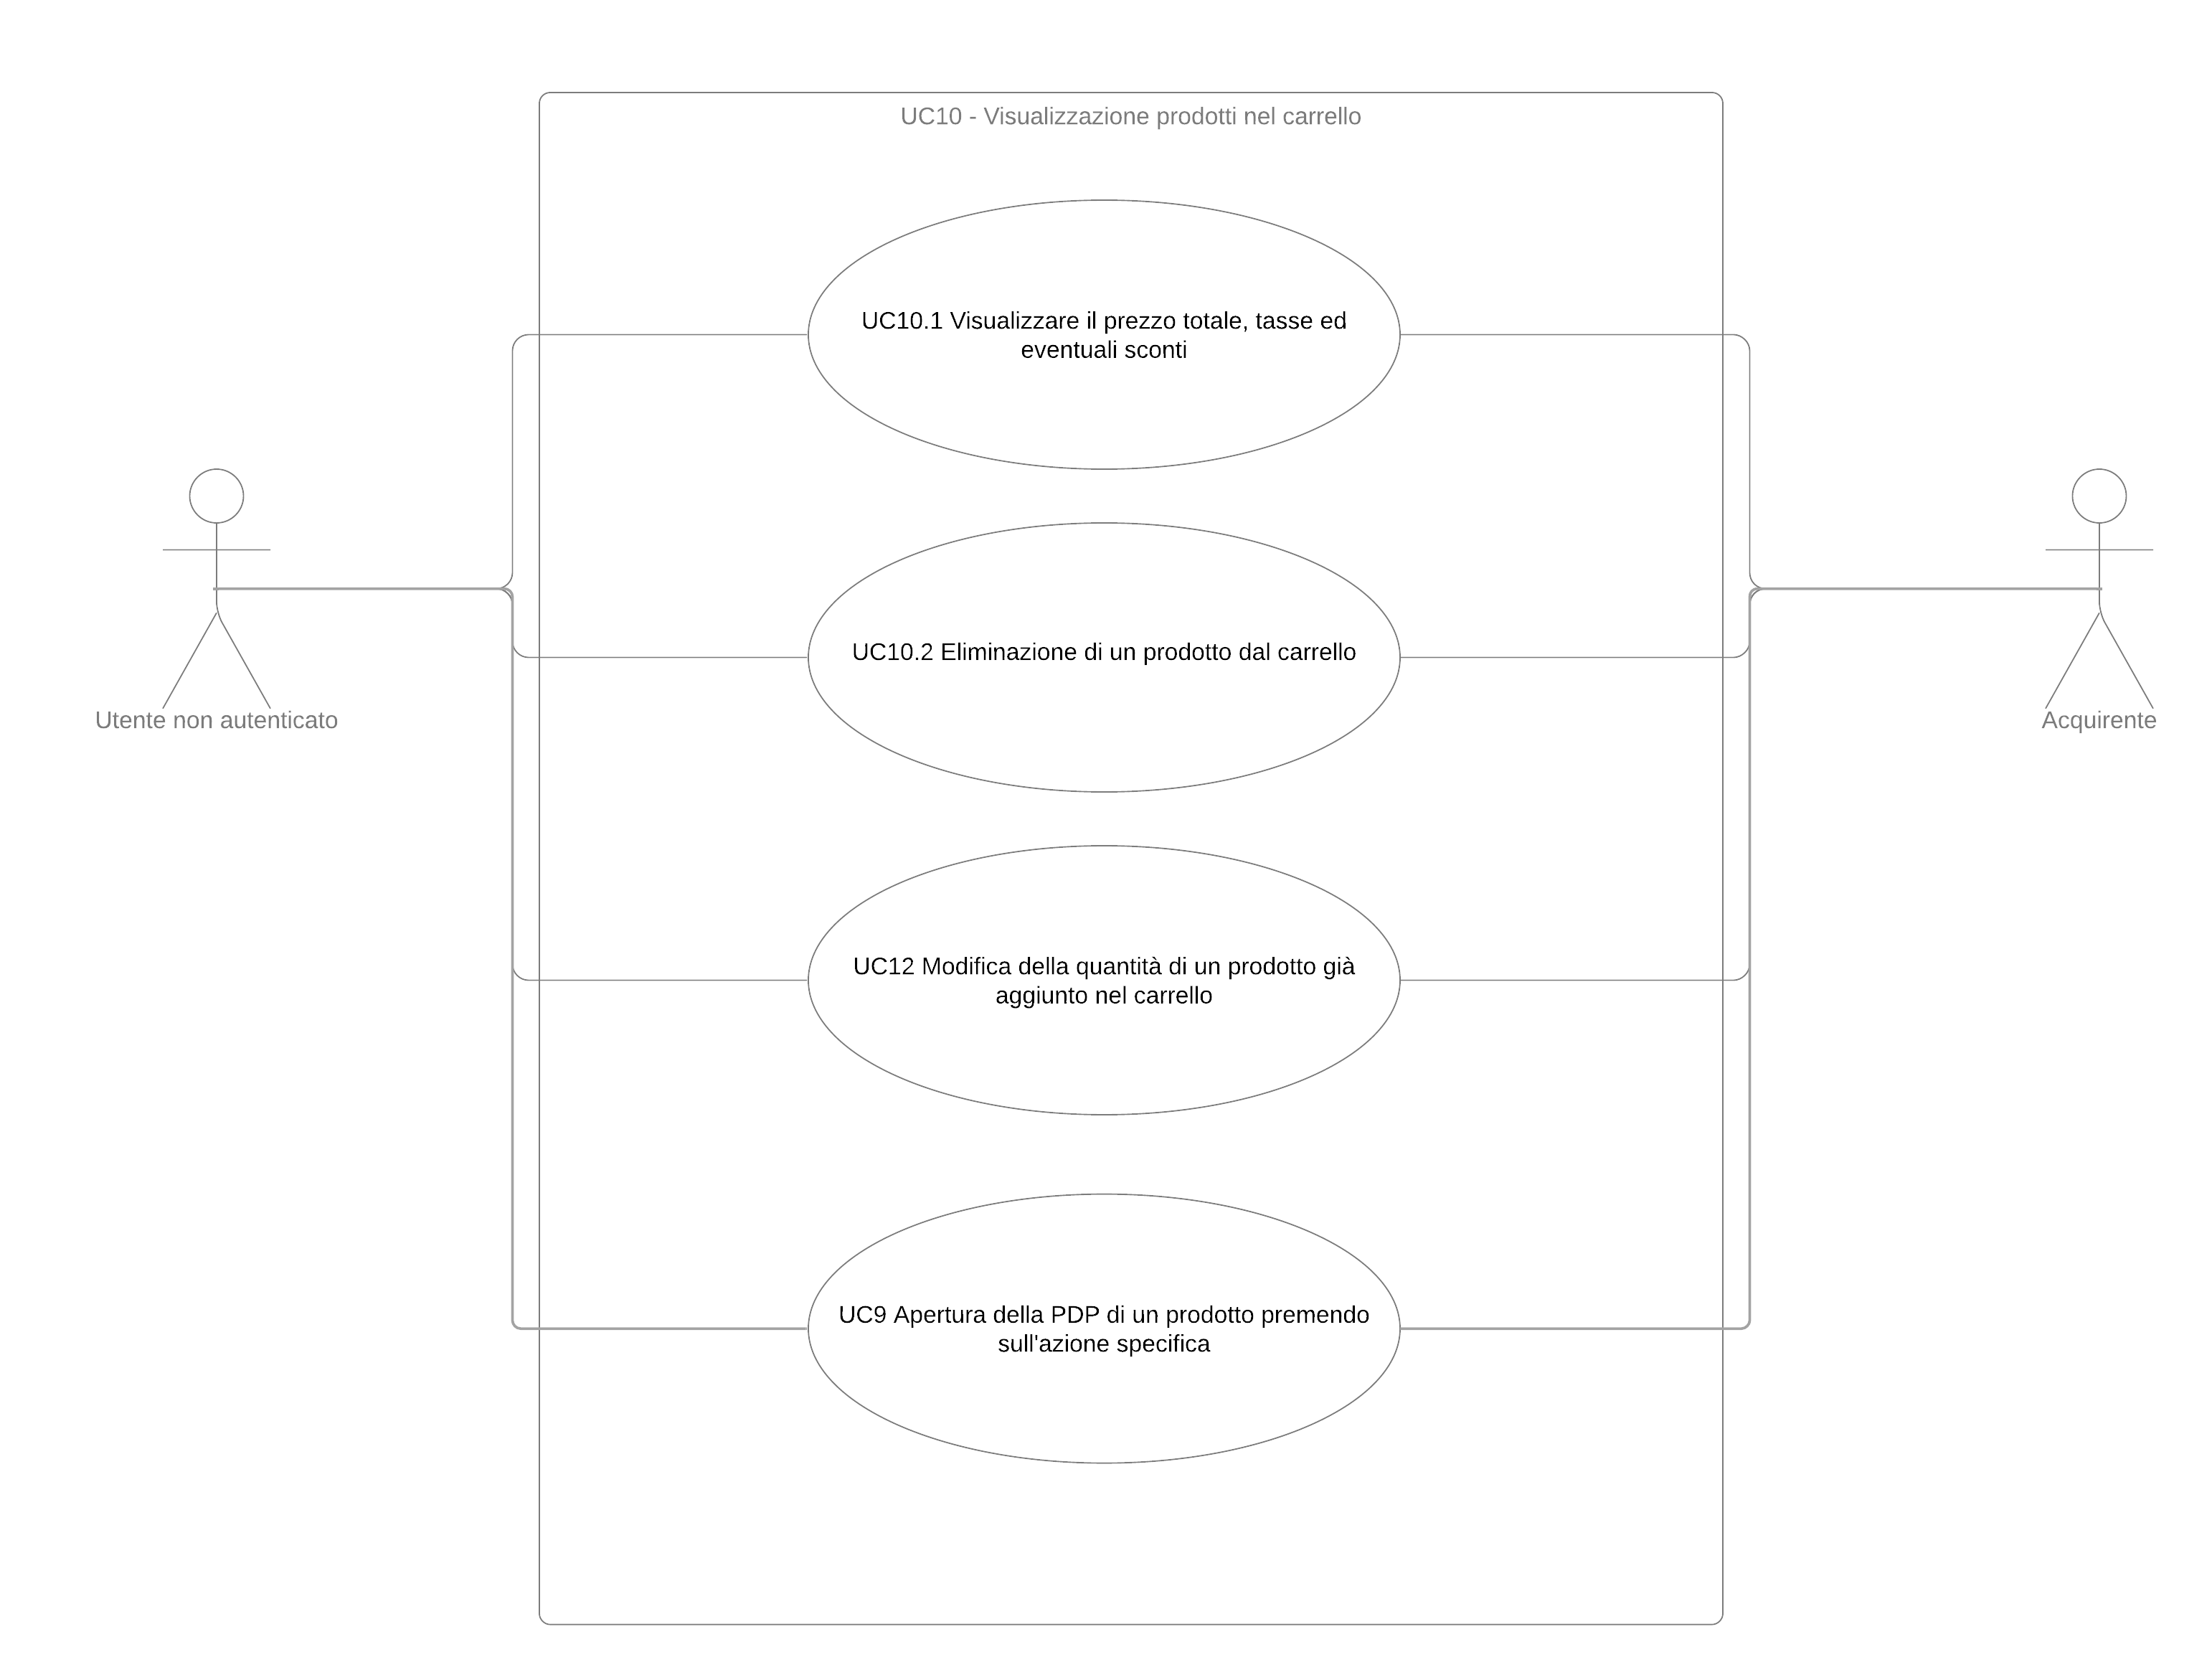
\includegraphics[width=\textwidth]{Immagini/DiagrammiUC/UC10VisualizzazioneProdottiNelCarrello.png}
%     \caption{Diagramma di \actualUC: Visualizzazione prodotti nel carrello} 
%     \label{fig:VisualizzazioneProdottiNelCarrello}
% \end{figure}

L'utente non autenticato o l'acquirente visualizza il proprio carrello.
\begin{itemize}
    \item \textbf{Attori primari:} acquirente o utente non autenticato;
    \item \textbf{Precondizione:} l'attore si trova in una qualunque schermata della piattaforma e seleziona la funzionalità per la visualizzazione del proprio carrello;
    \item \textbf{Postcondizione:} l'attore visualizza il proprio carrello con l'elenco dei prodotti presenti;
    \item \textbf{Scenario principale:} l'attore si trova in una qualunque schermata della piattaforma e seleziona la funzionalità per la visualizzazione del proprio carrello. In seguito visualizzerà il proprio carrello dove sarà presente il prezzo totale con l'elenco dei prodotti al suo interno. Per ogni prodotto sarà visualizzato:
    \begin{itemize}
        \item Prima foto disponibile del prodotto;
        \item Nome del prodotto;
        \item Quantità inserita;
        \item Prezzo del prodotto in base alla quantità inserita e agli sconti disponibili.
    \end{itemize}
    \item \textbf{Scenari alternativi:} 
    \begin{enumerate}[label=\lett]
        \item Se non sono stati inseriti dei prodotti all'interno del carrello, verrà visualizzato il messaggio "Carrello vuoto" e sarà data la possibilità all'attore di andare alla schermata principale per iniziare gli acquisti.
    \end{enumerate}
\end{itemize}

%%%%%%%%%%%%%%%%%%%%%%%%%%%%%%%%%%%%%%%%%%%%%%%%%%%%%%%%%%%%%%%%%%%%%%%%%%%%%%%%%%%%%%%%%%%%%%%%%%%%%%%%%%%%%%%%%%%%%%%%%%%%%%%%%%%%%%%%%%%%%%%%%%%%%%

\UC{Eliminazione di un prodotto dal carrello}
\label{eliminazione-prodotto-dal-carrello}

L'utente non autenticato o l'acquirente può eliminare un prodotto che ha inserito nel carrello.
\begin{itemize}
    \item \textbf{Attori primari:} acquirente o utente non autenticato;
    \item \textbf{Precondizione:} l'attore è nella pagina del carrello e ha inserito almeno un prodotto;
    \item \textbf{Postcondizione:} l'attore ha rimosso totalmente il prodotto dal carrello;
    \item \textbf{Scenario principale:} l'attore non vuole più ordinare un prodotto che ha aggiunto nel carrello per questo seleziona la funzionalità di eliminazione del prodotto dal carrello, il prodotto viene quindi rimosso totalmente dal carrello.
\end{itemize}

%%%%%%%%%%%%%%%%%%%%%%%%%%%%%%%%%%%%%%%%%%%%%%%%%%%%%%%%%%%%%%%%%%%%%%%%%%%%%%%%%%%%%%%%%%%%%%%%%%%%%%%%%%%%%%%%%%%%%%%%%%%%%%%%%%%%%%%%%%%%%%%%%%%%%%

\UC{Modifica della quantità di un prodotto nel carrello}
\label{modifica-quantita-nel-carrello}

L'utente non autenticato o l'acquirente modifica la quantità di un prodotto già nel carrello.
\begin{itemize}
    \item \textbf{Attori primari:} acquirente o utente non autenticato;
    \item \textbf{Precondizione:} l'attore è nella pagina del carrello dove ha inserito almeno un prodotto e ha selezionato la funzionalità di modifica della quantità di un prodotto;
    \item \textbf{Postcondizione:} la quantità del prodotto selezionato è stata modificata;
    \item \textbf{Scenario principale:} l'attore è nella pagina del carrello dove ha inserito almeno un prodotto e ha selezionato la funzionalità di modifica della quantità di un prodotto. In seguito la quantità di quel prodotto selezionato verrà modificata.
    \item \textbf{Estensioni:}
    \begin{enumerate}[label=\lett]
        \item L'attore modifica la quantità con una minore o uguale a zero. In questo caso:
        \begin{itemize}
            \item (UC\ref{estensione:quantita-da-aggiungere-al-carrello-non-valida}) - Viene visualizzato il messaggio d'errore quantità del prodotto non valida;
            \item Verrà impedita la modifica della quantità nel carrello.
        \end{itemize}
    \end{enumerate}
\end{itemize}

%%%%%%%%%%%%%%%%%%%%%%%%%%%%%%%%%%%%%%%%%%%%%%%%%%%%%%%%%%%%%%%%%%%%%%%%%%%%%%%%%%%%%%%%%%%%%%%%%%%%%%%%%%%%%%%%%%%%%%%%%%%%%%%%%%%%%%%%%%%%%%%%%%%%%%


% Checkout
%%%%%%%%%%%%%%%%%%%%%%%%%%%%%%%%%%%%%%%%%%%%%%%%%%%%%%%%%%%%%%%%%%%%%%%%%%%%%%%%%%%%%%%%%%%%%%%%%%%%%%%%%%%%%%%%%%%%%%%%%%%%%%%%%%%%%%%%%%%%%%%%%%%%%%%%%%%%%%%%%%%%%%%%%%%%%%

\UC{Checkout}

\begin{figure}[H]
    \centering
    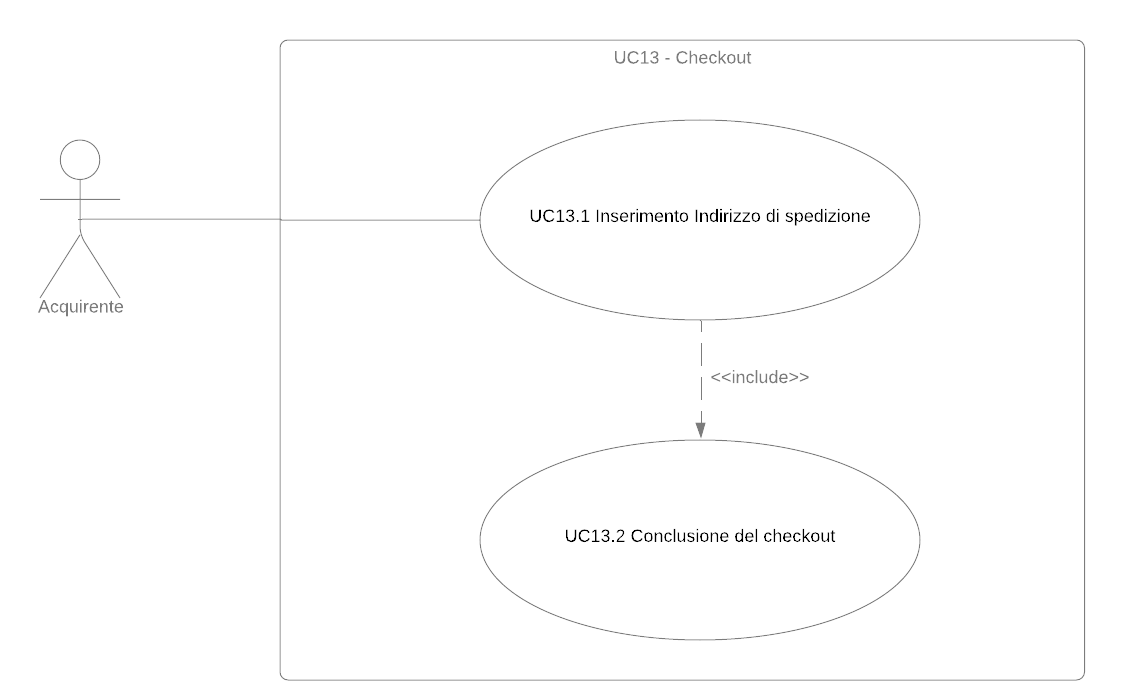
\includegraphics[scale=0.4]{Immagini/DiagrammiUC/UC13Checkout.png}
    \caption{Diagramma di \actualUC: Checkout} 
    \label{fig:Checkout}
\end{figure}

L'utente si trova nella schermata del carrello e vuole procedere al checkout per acquistare i prodotti scelti.
\begin{itemize}
    \item \textbf{Attori primari:} acquirente;
    \item \textbf{Attori secondari:} stripe;
    \item \textbf{Precondizione:} l'attore si trova nella schermata del carrello e ha selezionato l'azione di checkout;
    \item \textbf{Postcondizione:} l'attore ha terminato il checkout acquistando i prodotti nel carrello, il suo carrello risulterà vuoto e verrà reindirizzato alla schermata di riepilogo dell'ordine;
    \item \textbf{Scenario principale:} l'attore si trova nella schermata del carrello e seleziona la funzionalità per procedere con il checkout. In seguito eseguirà le seguenti azioni:
    \begin{itemize}
    	\item (\actualUC.1) - selezionare l'indirizzo di consegna;
    	\item (\actualUC.2) - selezionare la carta con la quale svolgere il pagamento;
    	\item inserire possibili informazioni aggiuntive per la consegna dell'acquisto;
        \item (\actualUC.3) - inviare il pagamento.
    \end{itemize}
    Se il pagamento è andato a buon fine, verrà visualizzato un messaggio il quale segnalerà la buona riuscita del pagamento e verrà visualizzata la schermata di riepilogo dell'ordine;
    \item \textbf{Estensioni:}
    \begin{enumerate}[label=\lett]
        \item se il pagamento fallisce per un errore di stripe:
        \begin{itemize}
            \item (UC) - verrà visualizzato il messaggio di errore pagamento non andato a buon fine;
            \item il carrello non verrà svuotato;
            \item l'acquirente verrà reindirizzato alla schermata del carrello.
        \end{itemize}
    \end{enumerate}
\end{itemize}

\resetSubUC

\subUC{Selezione dell'indirizzo della consegna}
L'acquirente seleziona l'indirizzo della consegna, ovvero dove verrà recapitato l'acquisto, tra gli indirizzi di consegna precedentemente inseriti.
\begin{itemize}
    \item \textbf{Attori primari:} acquirente;
    \item \textbf{Precondizione:} l'acquirente si trova durante la fase di checkout;
    \item \textbf{Postcondizione:} l'acquirente ha selezionato l'indirizzo di consegna;
    \item \textbf{Scenario principale:} l'acquirente si trova durante la fase di checkout e seleziona uno tra gli indirizzi di consegna precedentemente inseriti;
    \item \textbf{Scenari alternativi:}
    \begin{enumerate}[label=\lett]
        \item se sono presenti altri indirizzi, l'acquirente ha eseguito almeno un ordine e non seleziona alcun indirizzo per la consegna, allora verrà utilizzato l'indirizzo a cui è stato recapitato l'ultimo ordine;
        \item se non è presente alcun indirizzo da utilizzare per la consegna, allora verrà mostrato un messaggio il quale indicherà l'obbligo di dover inserire un indirizzo di consegna per poter proseguire con il checkout. In seguito l'indirizzo appena inserito verrà selezionato automaticamente per proseguire con la consegna.
    \end{enumerate}
\end{itemize}

\subUC{Selezione della carta per il pagamento}
L'acquirente seleziona la carta con la quale svolgere il pagamento tra quelle inserite precedentemente.
\begin{itemize}
    \item \textbf{Attori primari:} acquirente;
    \item \textbf{Precondizione:} l'acquirente si trova durante la fase di checkout;
    \item \textbf{Postcondizione:} l'acquirente ha selezionato la carta con la quale svolgere il pagamento;
    \item \textbf{Scenario principale:} l'acquirente si trova durante la fase di checkout e seleziona una tra le carte con la quale svolgere il pagamento tra quelle precedentemente inserite;
    \item \textbf{Scenari alternativi:}
    \begin{enumerate}[label=\lett]
        \item se sono presenti altre carte, l'acquirente ha eseguito almeno un ordine e non seleziona alcuna carta per il pagamento, allora verrà utilizzata la carta a cui è stato addebitato l'ultimo ordine;
        \item se non è presente alcuna carta da utilizzare per il pagamento, allora verrà mostrato un messaggio il quale indicherà l'obbligo di dover inserire una carta di pagamento per poter proseguire con il checkout. In seguito la carta appena inserita verrà selezionata automaticamente per proseguire con la consegna.
    \end{enumerate}
\end{itemize}

\subUC{Invio del pagamento}
L'acquirente procede al pagamento attraverso il servizio fornito da stripe.
\begin{itemize}
    \item \textbf{Attori primari:} acquirente;
    \item \textbf{Attori secondari:} stripe;
    \item \textbf{Precondizione:} l'acquirente è nella fase di checkout e ha selezionato indirizzo e carta con i quali proseguire al checkout;
    \item \textbf{Postcondizione:} l'acquirente ha effettuato il pagamento;
    \item \textbf{Scenario principale:} l'acquirente è nella fase di checkout, ha selezionato indirizzo e carta con i quali proseguire con il checkout e seleziona l'azione di invio del pagamento. A questo punto entrerà in gioco l'attore stripe che si occuperà del pagamento;
\end{itemize}

%%%%%%%%%%%%%%%%%%%%%%%%%%%%%%%%%%%%%%%%%%%%%%%%%%%%%%%%%%%%%%%%%%%%%%%%%%%%%%%%%%%%%%%%%%%%%%%%%%%%%%%%%%%%%%%%%%%%%%%%%%%%%%%%%%%%%%%%%%%%%%%%%%%%%%%%%%%%%%%%%%%%%%%%%%%%%%

%%%%%%%%%%%%%%%%%%%%%%%%%%%%%%%%%%%%%%%%%%%%%%%%%%%%%%%%%%%%%%%%%%%%%%%%%%%%%%%%%%%%%%%%%%%%%%%%%%%%%%%%%%%%%%%%%%%%%%%%%%%%%%%%%%%%%%%%%%%%%%%%%%%%%%%%%%%%%%%%%%%%%%%%%%%%%%

\UC{Inserimento nuovo indirizzo di consegna}
\label{inserimento-indirizzo-consegna}

L'acquirente vuole aggiungere un nuovo indirizzo di consegna.
\begin{itemize}
    \item \textbf{Attori primari:} acquirente;
    \item \textbf{Precondizione:} l'acquirente è nell'operazione di checkout e ha selezionato la funzione di aggiunta di un nuovo indirizzo per la consegna;
    \item \textbf{Postcondizione:} l'acquirente ha inserito il nuovo indirizzo di consegna;
    \item \textbf{Scenario principale:} l'acquirente è nell'operazione di checkout e vuole inserire un nuovo indirizzo di consegna. Per poterlo fare dovrà premere sull'azione di aggiunta nuovo indirizzo ed eseguire le seguenti azioni:
    \begin{itemize}
        \item (UC\ref{inserimento-indirizzo-consegna.modulo}) - Inserimento del nuovo indirizzo di consegna; 
        \item Confermare l'aggiunta del nuovo indirizzo di consegna.
    \end{itemize}
    \item \textbf{Scenari alternativi:}
    \begin{enumerate}[label=\lett]
        \item Se non viene confermata l'aggiunta del nuovo indirizzo di consegna, allora non verrà aggiunto e si andranno a perdere tutti i dati relativi ad esso che sono stati inseriti.
    \end{enumerate}
\end{itemize}

\subUC{Inserimento dei dati dell'indirizzo di consegna}
\label{inserimento-indirizzo-consegna.modulo}

L'acquirente compila il modulo per aggiungere un nuovo indirizzo di consegna.
\begin{itemize}
	\item \textbf{Attori primari:} acquirente;
	\item \textbf{Precondizione:} l'acquirente si trova nella schermata di aggiunta di un nuovo indirizzo di consegna;
	\item \textbf{Postcondizione:} l'acquirente ha compilato correttamente tutti i dati del nuovo indirizzo e può continuare con l'aggiunta;
	\item \textbf{Scenario principale:} l'acquirente compila i campi nel seguente modo:
	\begin{itemize}
		\item (UC\ref{inserimento-indirizzo-consegna.modulo.nazione}) - Selezione della nazione dell'indirizzo di consegna;
		\item (UC\ref{inserimento-indirizzo-consegna.modulo.comune}) - Inserimento del comune dell'indirizzo di consegna;
		\item (UC\ref{inserimento-indirizzo-consegna.modulo.via}) - Inserimento della via dell'indirizzo di consegna;
		\item (UC\ref{inserimento-indirizzo-consegna.modulo.cap}) - Inserimento del CAP dell'indirizzo di consegna.
	\end{itemize}
\end{itemize}

\subSubUC{Selezione della nazione dell'indirizzo di consegna}
\label{inserimento-indirizzo-consegna.modulo.nazione}

L'acquirente seleziona la nazione dell'indirizzo di consegna.
\begin{itemize}
    \item \textbf{Attori primari:} acquirente;
    \item \textbf{Precondizione:} l'acquirente si trova nella schermata di aggiunta di un nuovo indirizzo di consegna;
    \item \textbf{Postcondizione:} l'acquirente ha selezionato la nazione del nuovo indirizzo di consegna;
    \item \textbf{Scenario principale:} l'acquirente seleziona la nazione del nuovo indirizzo di consegna tra quelli disponibili;
    \item \textbf{Estensioni:}
    \begin{enumerate}[label=\lett]
        \item L'acquirente non seleziona alcuna nazione per il nuovo indirizzo di consegna. In questo caso:
        \begin{itemize}
            \item (UC\ref{estensione:campo-obbligatorio-non-inserito}) - Viene mostrato il messaggio d'errore campo dati obbligatorio non inserito;
            \item Verrà impedita l'aggiunta del nuovo indirizzo.
        \end{itemize}
    \end{enumerate}
\end{itemize}

\subSubUC{Inserimento del comune dell'indirizzo di consegna}
\label{inserimento-indirizzo-consegna.modulo.comune}

L'acquirente inserisce il comune dell'indirizzo di consegna.
\begin{itemize}
    \item \textbf{Attori primari:} acquirente;
    \item \textbf{Precondizione:} l'acquirente si trova nella schermata di aggiunta di un nuovo indirizzo di consegna;
    \item \textbf{Postcondizione:} l'acquirente ha inserito il comune del nuovo indirizzo di consegna;
    \item \textbf{Scenario principale:} l'acquirente inserisce correttamente il comune del nuovo indirizzo di consegna;
    \item \textbf{Estensioni:}
    \begin{enumerate}[label=\lett]
        \item L'acquirente non inserisce alcun comune per il nuovo indirizzo di consegna. In questo caso:
        \begin{itemize}
            \item (UC\ref{estensione:campo-obbligatorio-non-inserito}) - Viene mostrato il messaggio d'errore campo dati obbligatorio non inserito;
            \item Verrà impedita l'aggiunta del nuovo indirizzo.
        \end{itemize}
        \item L'acquirente inserisce dei caratteri non alfabetici. In questo caso:
        \begin{itemize}
            \item (UC\ref{estensione:caratteri-non-alfabetici-non-permessi}) - Viene mostrato il messaggio d'errore caratteri non alfabetici non permessi;
            \item Verrà impedita l'aggiunta dell'indirizzo di consegna.
        \end{itemize}
    \end{enumerate}
\end{itemize}

\subSubUC{Inserimento della via dell'indirizzo di consegna}
\label{inserimento-indirizzo-consegna.modulo.via}

L'acquirente inserisce la via dell'indirizzo di consegna, includendo anche il numero civico e l'eventuale interno.
\begin{itemize}
    \item \textbf{Attori primari:} acquirente;
    \item \textbf{Precondizione:} l'acquirente si trova nella schermata di aggiunta di un nuovo indirizzo di consegna;
    \item \textbf{Postcondizione:} l'acquirente ha inserito la via del nuovo indirizzo di consegna;
    \item \textbf{Scenario principale:} l'acquirente inserisce correttamente la via del nuovo indirizzo di consegna;
    \item \textbf{Estensioni:}
    \begin{enumerate}[label=\lett]
        \item L'acquirente non inserisce alcuna via per il nuovo indirizzo di consegna. In questo caso:
        \begin{itemize}
            \item (UC\ref{estensione:campo-obbligatorio-non-inserito}) - Viene mostrato il messaggio d'errore campo dati obbligatorio non inserito;
            \item Verrà impedita l'aggiunta del nuovo indirizzo.
        \end{itemize}
    \end{enumerate}
\end{itemize}

\subSubUC{Inserimento del CAP dell'indirizzo di consegna}
\label{inserimento-indirizzo-consegna.modulo.cap}

L'acquirente inserisce il CAP dell'indirizzo di consegna.
\begin{itemize}
    \item \textbf{Attori primari:} acquirente;
    \item \textbf{Precondizione:} l'acquirente si trova nella schermata di aggiunta di un nuovo indirizzo di consegna;
    \item \textbf{Postcondizione:} l'acquirente ha inserito il CAP del nuovo indirizzo di consegna;
    \item \textbf{Scenario principale:} l'acquirente inserisce correttamente il CAP del nuovo indirizzo di consegna;
    \item \textbf{Estensioni:}
    \begin{enumerate}[label=\lett]
        \item L'acquirente non inserisce alcun CAP per il nuovo indirizzo di consegna. In questo caso:
        \begin{itemize}
            \item (UC\ref{estensione:campo-obbligatorio-non-inserito}) - Viene mostrato il messaggio d'errore campo dati obbligatorio non inserito;
            \item Verrà impedita l'aggiunta del nuovo indirizzo.
        \end{itemize}
        \item L'acquirente non inserisce esattamente 5 numeri come CAP. In questo caso:
        \begin{itemize}
            \item (UC\ref{estensione:cap-non-valido}) - Viene mostrato il messaggio d'errore CAP non valido;
            \item Verrà impedita l'aggiunta del nuovo indirizzo.
        \end{itemize}
    \end{enumerate}
\end{itemize}

%%%%%%%%%%%%%%%%%%%%%%%%%%%%%%%%%%%%%%%%%%%%%%%%%%%%%%%%%%%%%%%%%%%%%%%%%%%%%%%%%%%%%%%%%%%%%%%%%%%%%%%%%%%%%%%%%%%%%%%%%%%%%%%%%%%%%%%%%%%%%%%%%%%%%%%%%%%%%%%%%%%%%%%%%%%%%%

\UC{Modifica indirizzo di consegna}
\label{modifica-indirizzo-consegna}

L'acquirente è nell'operazione di checkout e vuole modificare un indirizzo di consegna precedentemente inserito.
\begin{itemize}
    \item \textbf{Attori primari:} acquirente;
    \item \textbf{Precondizione:} l'acquirente è nell'operazione di checkout e ha selezionato la funzione di modifica di un indirizzo per la consegna precedentemente inserito;
    \item \textbf{Postcondizione:} l'acquirente ha modificato l'indirizzo di consegna desiderata;
    \item \textbf{Scenario principale:} l'acquirente è nell'operazione di checkout e vuole modificare i dati di un indirizzo di consegna precedentemente inserito. Le informazioni che potranno essere modificate sono:
    \begin{itemize}
        \item (UC\ref{modifica-indirizzo-consegna.nazione}) - Modifica della nazione dell'indirizzo di consegna;
		\item (UC\ref{modifica-indirizzo-consegna.comune}) - Modifica del comune dell'indirizzo di consegna;
		\item (UC\ref{modifica-indirizzo-consegna.via}) - Modifica della via dell'indirizzo di consegna;
		\item (UC\ref{modifica-indirizzo-consegna.cap}) - Modifica del CAP dell'indirizzo di consegna.
    \end{itemize}
    In seguito ci sarà la conferma delle modifiche compiute e i dati dell'indirizzo di consegna verranno modificati.
    \item \textbf{Scenari alternativi:}
    \begin{enumerate}[label=\lett]
        \item Se non vengono confermate le modifiche compiute, allora non verranno applicate e andranno perse.
    \end{enumerate}
\end{itemize}

\subUC{Modifica della nazione dell'indirizzo di consegna}
\label{modifica-indirizzo-consegna.nazione}

L'acquirente vuole modificare la nazione dell'indirizzo di consegna.
\begin{itemize}
    \item \textbf{Attori primari:} acquirente;
    \item \textbf{Precondizione:} l'acquirente si trova nella schermata di modifica di un indirizzo di consegna precedentemente inserito;
    \item \textbf{Postcondizione:} l'acquirente ha modificato la nazione dell'indirizzo di consegna;
    \item \textbf{Scenario principale:} l'acquirente modifica correttamente la nazione dell'indirizzo di consegna, selezionandone uno tra quelli disponibili;
    \item \textbf{Scenari alternativi:}
    \begin{enumerate}[label=\lett]
        \item L'acquirente non modifica la nazione dell'indirizzo di consegna attuale e, per questo, non verrà modificato.
    \end{enumerate}
\end{itemize}

\subUC{Modifica del comune dell'indirizzo di consegna}
\label{modifica-indirizzo-consegna.comune}

L'acquirente vuole modificare il comune dell'indirizzo di consegna.
\begin{itemize}
    \item \textbf{Attori primari:} acquirente;
    \item \textbf{Precondizione:} l'acquirente si trova nella schermata di modifica di un indirizzo di consegna precedentemente inserito;
    \item \textbf{Postcondizione:} l'acquirente ha modificato il comune dell'indirizzo di consegna;
    \item \textbf{Scenario principale:} l'acquirente modifica correttamente il comune dell'indirizzo di consegna attraverso le seguenti azioni:
    \begin{itemize}
        \item Si posiziona nel campo dove è presente l'attuale comune dell'indirizzo di consegna;
        \item Modifica il comune dell'indirizzo di consegna.
    \end{itemize}
    \item \textbf{Scenari alternativi:}
    \begin{enumerate}[label=\lett]
        \item L'acquirente non modifica il comune dell'indirizzo di consegna attuale e, per questo, non verrà modificato.
    \end{enumerate}
    \item \textbf{Estensioni:}
    \begin{enumerate}[label=\lett]
        \item L'acquirente elimina l'attuale comune dell'indirizzo di consegna e non ne inserisce uno nuovo. In questo caso:
        \begin{itemize}
            \item (UC\ref{estensione:campo-obbligatorio-non-inserito}) - Viene mostrato il messaggio d'errore campo dati obbligatorio non inserito;
            \item Verrà impedita la modifica dell'indirizzo di consegna.
        \end{itemize}
        \item L'acquirente modifica il comune dell'indirizzo di consegna inserendo dei caratteri non alfabetici. In questo caso:
        \begin{itemize}
            \item (UC\ref{estensione:caratteri-non-alfabetici-non-permessi}) - Viene mostrato il messaggio d'errore caratteri non alfabetici non permessi;
            \item Verrà impedita la modifica dell'indirizzo di consegna.
        \end{itemize}
    \end{enumerate}
\end{itemize}

\subUC{Modifica della via dell'indirizzo di consegna}
\label{modifica-indirizzo-consegna.via}

L'acquirente vuole modificare la via dell'indirizzo di consegna.
\begin{itemize}
    \item \textbf{Attori primari:} acquirente;
    \item \textbf{Precondizione:} l'acquirente si trova nella schermata di modifica di un indirizzo di consegna precedentemente inserito;
    \item \textbf{Postcondizione:} l'acquirente ha modificato la via dell'indirizzo di consegna;
    \item \textbf{Scenario principale:} l'acquirente modifica correttamente la via dell'indirizzo di consegna attraverso le seguenti azioni:
    \begin{itemize}
        \item Si posiziona nel campo dove è presente l'attuale via dell'indirizzo di consegna;
        \item Modifica la via dell'indirizzo di consegna.
    \end{itemize}
    \item \textbf{Scenari alternativi:}
    \begin{enumerate}[label=\lett]
        \item L'acquirente non modifica la via dell'indirizzo di consegna attuale e, per questo, non verrà modificata.
    \end{enumerate}
    \item \textbf{Estensioni:}
    \begin{enumerate}[label=\lett]
        \item L'acquirente elimina l'attuale via dell'indirizzo di consegna e non ne inserisce una nuova. In questo caso:
        \begin{itemize}
            \item (UC\ref{estensione:campo-obbligatorio-non-inserito}) - Viene mostrato il messaggio d'errore campo dati obbligatorio non inserito;
            \item Verrà impedita la modifica dell'indirizzo di consegna.
        \end{itemize}
    \end{enumerate}
\end{itemize}

\subUC{Modifica del CAP dell'indirizzo di consegna}
\label{modifica-indirizzo-consegna.cap}

L'acquirente vuole modificare il CAP dell'indirizzo di consegna.
\begin{itemize}
    \item \textbf{Attori primari:} acquirente;
    \item \textbf{Precondizione:} l'acquirente si trova nella schermata di modifica di un indirizzo di consegna precedentemente inserito;
    \item \textbf{Postcondizione:} l'acquirente ha modificato il CAP dell'indirizzo di consegna;
    \item \textbf{Scenario principale:} l'acquirente modifica correttamente il CAP dell'indirizzo di consegna attraverso le seguenti azioni:
    \begin{itemize}
        \item Si posiziona nel campo dove è presente l'attuale CAP dell'indirizzo di consegna;
        \item Modifica il CAP dell'indirizzo di consegna.
    \end{itemize}
    \item \textbf{Scenari alternativi:}
    \begin{enumerate}[label=\lett]
        \item L'acquirente non modifica il CAP dell'indirizzo di consegna attuale e, per questo, non verrà modificato.
    \end{enumerate}
    \item \textbf{Estensioni:}
    \begin{enumerate}[label=\lett]
        \item L'acquirente elimina l'attuale CAP dell'indirizzo di consegna e non ne inserisce uno nuovo. In questo caso:
        \begin{itemize}
            \item (UC\ref{estensione:campo-obbligatorio-non-inserito}) - Viene mostrato il messaggio d'errore campo dati obbligatorio non inserito;
            \item Verrà impedita la modifica dell'indirizzo di consegna.
        \end{itemize}
        \item L'acquirente modifica il CAP in modo tale che non sia composto da esattamente 5 numeri. In questo caso:
        \begin{itemize}
            \item (UC\ref{estensione:cap-non-valido}) - Viene mostrato il messaggio d'errore CAP non valido;
            \item Verrà impedita la modifica dell'indirizzo di consegna.
        \end{itemize}
    \end{enumerate}
\end{itemize}

%%%%%%%%%%%%%%%%%%%%%%%%%%%%%%%%%%%%%%%%%%%%%%%%%%%%%%%%%%%%%%%%%%%%%%%%%%%%%%%%%%%%%%%%%%%%%%%%%%%%%%%%%%%%%%%%%%%%%%%%%%%%%%%%%%%%%%%%%%%%%%%%%%%%%%%%%%%%%%%%%%%%%%%%%%%%%%

\UC{Eliminazione indirizzo di consegna}
\label{eliminazione-indirizzo-consegna}

L'acquirente vuole eliminare un indirizzo di consegna precedentemente inserito.
\begin{itemize}
    \item \textbf{Attori primari:} acquirente;
    \item \textbf{Precondizione:}  l'acquirente è nell'operazione di checkout;
    \item \textbf{Postcondizione:} l'acquirente ha eliminato l'indirizzo di consegna desiderato.
    \item \textbf{Scenario principale:} l'acquirente è nell'operazione di checkout e vuole eliminare un indirizzo di consegna precedentemente inserito. Per poterlo fare dovrà svolgere le seguenti azioni:
    \begin{itemize}
        \item Seleziona l'indirizzo di consegna da eliminare;
        \item Confermare l'eliminazione della carta.
    \end{itemize}
    Se l'indirizzo di consegna eliminato è quella attualmente selezionato per la consegna e ci sono altri indirizzi di consegna inseriti, allora verrà selezionato per il proseguimento della consegna l'indirizzo successivo. Se viene eliminato l'ultimo indirizzo di consegna e quindi non esiste un indirizzo successivo, verrà selezionato il primo;
    \item \textbf{Scenari alternativi:}
    \begin{enumerate}[label=\lett]
        \item L'acquirente non conferma l'eliminazione dell'indirizzo di consegna e, per questo motivo, non verrà eliminato;
        \item Se l'indirizzo di consegna eliminato dall'acquirente è l'unico attualmente inserito, allora verrà mostrato un messaggio con l'obbligo di dover inserire un nuovo indirizzo di consegna per poter proseguire con il checkout.
    \end{enumerate}
\end{itemize}

%%%%%%%%%%%%%%%%%%%%%%%%%%%%%%%%%%%%%%%%%%%%%%%%%%%%%%%%%%%%%%%%%%%%%%%%%%%%%%%%%%%%%%%%%%%%%%%%%%%%%%%%%%%%%%%%%%%%%%%%%%%%%%%%%%%%%%%%%%%%%%%%%%%%%%%%%%%%%%%%%%%%%%%%%%%%%%

% Ordini
%%%%%%%%%%%%%%%%%%%%%%%%%%%%%%%%%%%%%%%%%%%%%%%%%%%%%%%%%%%%%%%%%%%%%%%%%%%%%%%%%%%%%%%%%%

\UC{Visualizzazione ordini effettuati}
L'acquirente può visualizzare l'elenco degli ordini effettuati sulla piattaforma.
\begin{itemize}
    \item \textbf{Attori primari:} acquirente;
    \item \textbf{Precondizione:} l'acquirente si trova in una qualsiasi altra schermata e seleziona l'azione per accedere all'elenco degli ordini effettuati sulla piattaforma;
    \item \textbf{Postcondizione:} l'acquirente visualizza l'elenco degli ordini effettuati sulla piattaforma in ordine cronologico decrescente;
    \item \textbf{Scenario principale:} l'acquirente si trova in una qualsiasi altra schermata e seleziona l'azione per accedere all'elenco degli ordini effettuati sulla piattaforma. In seguito visualizzerà l'elenco degli ordini effettuati sulla piattaforma, dove è indicato per ogni ordine:
    \begin{itemize}
        \item Se è stato evaso o no;
        \item Il prezzo totale che è stato pagato;
        \item L'indirizzo a cui è stato consegnato o verrà consegnato;
        \item Una lista di tutti i prodotti acquistati in quell'ordine, dove per ogni prodotto verrà visualizzato:
        \begin{itemize}
            \item Nome del prodotto;
            \item Quantità acquistata;
            \item Prezzo totale del prodotto per la quantità.
        \end{itemize}
    \end{itemize}
    \item \textbf{Scenari alternativi:} 
    \begin{enumerate}[label=\lett]
        \item L'acquirente non ha ancora effettuato ordini, viene visualizzato il messaggio "Nessun ordine effettuato" e sarà data la possibilità all'acquirente di tornare alla home per iniziare gli acquisti.
    \end{enumerate}
\end{itemize}

%%%%%%%%%%%%%%%%%%%%%%%%%%%%%%%%%%%%%%%%%%%%%%%%%%%%%%%%%%%%%%%%%%%%%%%%%%%%%%%%%%%%%%%%%%

\UC{Filtro temporale per gli ordini effettuati}
L'acquirente filtra temporalmente l'elenco degli ordini effettuati sulla piattaforma.
\begin{itemize}
    \item \textbf{Attori primari:} acquirente;
    \item \textbf{Precondizione:} l'acquirente si trova nella schermata di visualizzazione degli ordini effettuati;
    \item \textbf{Postcondizione:} l'acquirente visualizzerà tutti gli ordini che sono stati fatti tra la data di iniziale e quella finale;
    \item \textbf{Scenario principale:} l'acquirente si trova nella schermata di visualizzazione degli ordini effettuati e vuole filtrare gli ordini secondo un intervallo temporale. Per farlo dovrà:
    \begin{itemize}
        \item (\actualUC.1) - Impostazione della data iniziale dell'intervallo temporale;
        \item (\actualUC.2) - Impostazione della data finale dell'intervallo temporale.
    \end{itemize}
    \item \textbf{Estensioni:}
    \begin{enumerate}[label=\lett]
        \item L'acquirente imposta un intervallo temporale nel quale non sono stati effettuati ordini. In questo caso:
        \begin{itemize}
            \item (UC) - Verrà visualizzato il messaggio nessun ordine effettuato nell'arco temporale impostato.
        \end{itemize}
    \end{enumerate}
\end{itemize}

\resetSubUC

\subUC{Impostazione della data iniziale dell'intervallo temporale}
L'acquirente imposta la data iniziale dell'intervallo per il quale filtrare l'elenco degli ordini effettuati sulla piattaforma.
\begin{itemize}
    \item \textbf{Attori primari:} acquirente;
    \item \textbf{Precondizione:} l'acquirente si trova nella schermata di visualizzazione degli ordini effettuati;
    \item \textbf{Postcondizione:} l'acquirente ha impostato la data iniziale dell'intervallo per la quale filtrare l'elenco degli ordini effettuati sulla piattaforma;
    \item \textbf{Scenario principale:} l'acquirente si trova nella schermata di visualizzazione degli ordini effettuati e inserisce una data valida e minore o uguale a quella finale, come data iniziale dell'intervallo per la quale filtrare l'elenco degli ordini effettuati;
    \item \textbf{Estensioni:}
    \begin{enumerate}[label=\lett]
        \item L'acquirente inserisce una data iniziale non nel formato corretto. In questo caso:
        \begin{itemize}
            \item (UC) - Verrà visualizzato il messaggio d'errore data non valida;
            \item Non verrà eseguita la ricerca.
        \end{itemize} 
        \item L'acquirente inserisce una data iniziale maggiore di quella finale. In questo caso:
        \begin{itemize}
            \item (UC) - Verrà visualizzato il messaggio d'errore data iniziale maggiore di quella finale;
            \item Non verrà eseguita la ricerca.
        \end{itemize}
    \end{enumerate}
\end{itemize}

\subUC{Impostazione della data finale dell'intervallo temporale}
L'acquirente imposta la data finale dell'intervallo per il quale filtrare l'elenco degli ordini effettuati sulla piattaforma.
\begin{itemize}
    \item \textbf{Attori primari:} acquirente;
    \item \textbf{Precondizione:} l'acquirente si trova nella schermata di visualizzazione degli ordini effettuati;
    \item \textbf{Postcondizione:} l'acquirente ha impostato la data finale dell'intervallo per la quale filtrare l'elenco degli ordini effettuati sulla piattaforma;
    \item \textbf{Scenario principale:} l'acquirente si trova nella schermata di visualizzazione degli ordini effettuati e inserisce una data valida e maggiore o uguale di quella iniziale, come data finale dell'intervallo per la quale filtrare l'elenco degli ordini effettuati;
    \item \textbf{Estensioni:}
    \begin{enumerate}[label=\lett]
        \item L'acquirente inserisce una data finale non nel formato corretto. In questo caso:
        \begin{itemize}
            \item (UC) - Verrà visualizzato il messaggio d'errore data non valida;
            \item Non verrà eseguita la ricerca.
        \end{itemize} 
        \item L'acquirente inserisce una data finale minore di quella iniziale. In questo caso:
        \begin{itemize}
            \item (UC) - Verrà visualizzato il messaggio d'errore data finale minore di quella iniziale;
            \item Non verrà eseguita la ricerca.
        \end{itemize}
    \end{enumerate}
\end{itemize}

    
% Gestione account acquirente
%%%%%%%%%%%%%%%%%%%%%%%%%%%%%%%%%%%%%%%%%%%%%%%%%%%%%%%%%%%%%%%%%%%%%%%%%%%%%%%%%%%%%%%%%%%%%%%%%%%%%%%%%%%%%%%%%

\UC{Modifica informazioni acquirente}
\label{modifica-informazioni-acquirente}

\begin{figure}[H]
    \centering
    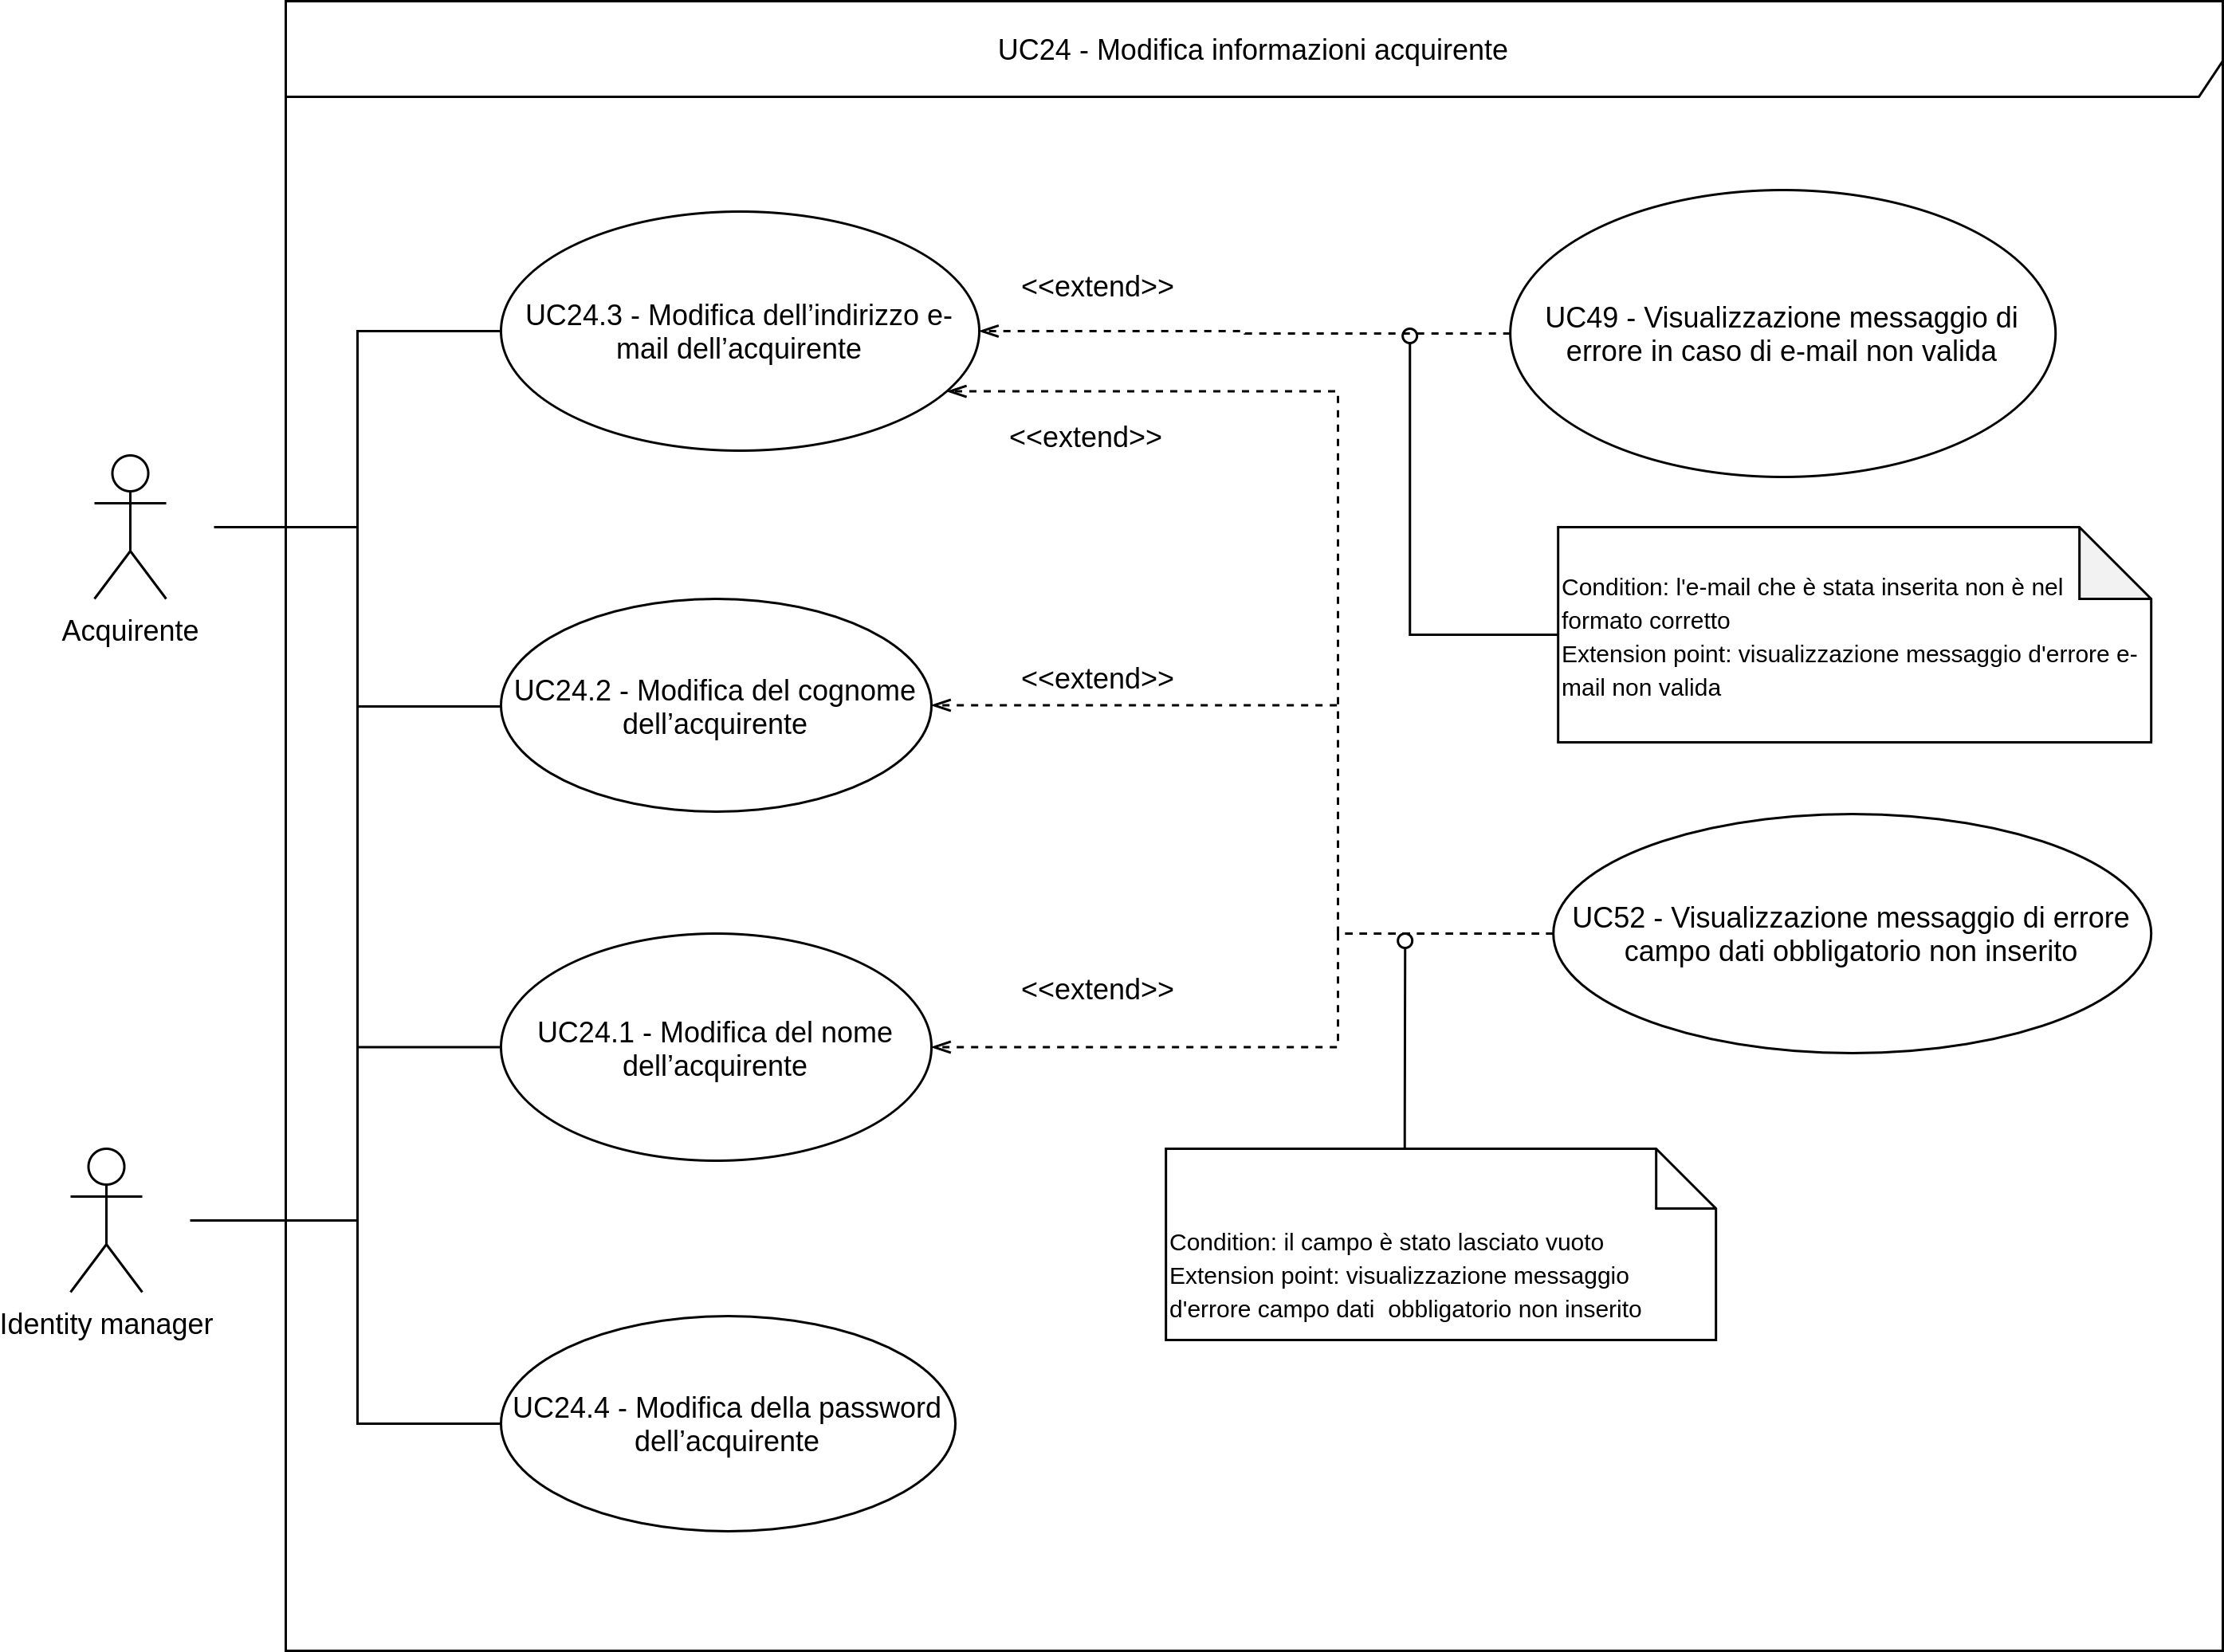
\includegraphics[scale=0.6]{Immagini/DiagrammiUC/Acquirente/ModificaInformazioniAcquirente.png}
    \caption{Diagramma di \actualUC: Modifica informazioni acquirente}
    \label{fig:modifica-informazioni-acquirente}
\end{figure}

L'acquirente può modificare le sue informazioni personali.
\begin{itemize}
    \item \textbf{Attori primari:} acquirente;
    \item \textbf{Attori secondari:} identity manager;
    \item \textbf{Precondizione:} l'acquirente si trova nella vista di modifica informazioni personali;
    \item \textbf{Postcondizione:} l'acquirente ha aggiornato le sue informazioni personali;
    \item \textbf{Scenario principale:} l'acquirente ha selezionato la funzionalità prevista per la modifica delle informazioni personali e, dopo aver compiuto la modifica, potrà confermarla attraverso la funzione di salvataggio. Le informazioni che si possono modificare sono:
    \begin{itemize}
        \item (UC\ref{modifica-informazioni-acquirente.nome}) - Modifica del nome dell'acquirente;
        \item (UC\ref{modifica-informazioni-acquirente.cognome}) - Modifica del cognome dell'acquirente;
        \item (UC\ref{modifica-informazioni-acquirente.email}) - Modifica dell'indirizzo e-mail dell'acquirente;
        \item (UC\ref{modifica-password}) - Modifica della password.
    \end{itemize}
    In seguito ci sarà la conferma delle modifiche compiute e le informazioni personali verranno modificate;
    \item \textbf{Scenari alternativi:}
    \begin{enumerate}[label=\lett]
        \item L'acquirente non conferma le modifiche effettuate, perciò non verranno modificate le informazioni personali.
    \end{enumerate}
    \item \textbf{Estensioni:} 
    \begin{enumerate}[label=\lett]
        \item L'acquirente modifica la propria e-mail con una già utilizzata nella piattaforma e l'identity manager lo segnala. In questo caso:
        \begin{itemize}
            \item L'identity manager segnala che le due password inserite non coincidono;
            \item (UC\ref{estensione:cambio-con-email-esistente}) - Verrà visualizzato il messaggio di errore in caso di cambio e-mail con una già utilizzata nella piattaforma;
            \item Verrà impedita la modifica delle informazioni.
        \end{itemize}
        \item L'acquirente inserisce una password di conferma diversa da quella inserita nel campo di inserimento nuova password e l'identity manager lo segnala. In questo caso:
        \begin{itemize}
            \item (UC\ref{estensione:password-conferma-diverse}) - Verrà visualizzato il messaggio di errore di password e password di conferma diverse;
            \item Verrà impedita la modifica delle informazioni.
        \end{itemize}
    \end{enumerate}
\end{itemize}

\subUC{Modifica del nome dell'acquirente}
\label{modifica-informazioni-acquirente.nome}

L'acquirente modifica il proprio nome.
\begin{itemize}
    \item \textbf{Attori primari:} acquirente;
    \item \textbf{Attori secondari:} identity manager;
    \item \textbf{Precondizione:} l'acquirente si trova nella schermata di modifica informazioni personali e vuole modificare il proprio nome;
    \item \textbf{Postcondizione:} l'acquirente ha aggiornato il proprio nome sulla piattaforma;
    \item \textbf{Scenario principale:} l'acquirente si trova nella schermata di modifica informazioni personali e vuole modificare il proprio nome attraverso le seguenti azioni:
        \begin{itemize}
            \item Si posiziona nel campo di inserimento del nome dove è presente quello attualmente utilizzata;
            \item Cambia il nome attuale modificandolo o inserendone uno completamente nuovo.
        \end{itemize}
    \item \textbf{Scenari alternativi:} 
    \begin{enumerate}[label=\lett]
        \item L'acquirente non modifica il proprio nome attuale e per questo non cambierà.
    \end{enumerate}
    \item \textbf{Estensioni:} 
    \begin{enumerate}[label=\lett]
        \item L'acquirente elimina il proprio nome attuale, non ne inserisce uno nuovo e l'identity manager lo segnala. In questo caso:
        \begin{itemize}
            \item (UC\ref{estensione:campo-obbligatorio-non-inserito}) - Verrà visualizzato il messaggio di errore campo dati obbligatorio non inserito;
            \item Verrà impedita la modifica delle informazioni.
        \end{itemize}
    \end{enumerate}
\end{itemize}

\subUC{Modifica del cognome dell'acquirente}
\label{modifica-informazioni-acquirente.cognome}

L'acquirente modifica il proprio cognome.
\begin{itemize}
    \item \textbf{Attori primari:} acquirente;
    \item \textbf{Attori secondari:} identity manager;
    \item \textbf{Precondizione:} l'acquirente si trova nella schermata di modifica informazioni personali e vuole modificare il proprio cognome;
    \item \textbf{Postcondizione:} l'acquirente ha aggiornato il proprio cognome sulla piattaforma;
    \item \textbf{Scenario principale:} l'acquirente si trova nella schermata di modifica informazioni personali e vuole modificare il proprio cognome attraverso le seguenti azioni:
        \begin{itemize}
            \item Si posiziona nel campo di inserimento del cognome dove è presente quello attualmente utilizzata;
            \item Cambia il cognome attuale modificandolo o inserendone uno completamente nuovo.
        \end{itemize}
    \item \textbf{Scenari alternativi:} 
    \begin{enumerate}[label=\lett]
        \item L'acquirente non modifica il proprio cognome attuale e per questo non cambierà.
    \end{enumerate}
    \item \textbf{Estensioni:} 
    \begin{enumerate}[label=\lett]
        \item L'acquirente elimina il proprio cognome attuale, non ne inserisce uno nuovo e l'identity manager lo segnala. In questo caso:
        \begin{itemize}
            \item (UC\ref{estensione:campo-obbligatorio-non-inserito}) - Verrà visualizzato il messaggio di errore campo dati obbligatorio non inserito;
            \item Verrà impedita la modifica delle informazioni.
        \end{itemize}
    \end{enumerate}
\end{itemize}

\subUC{Modifica dell'indirizzo e-mail dell'acquirente}
\label{modifica-informazioni-acquirente.email}

L'acquirente modifica la propria e-mail.
\begin{itemize}
    \item \textbf{Attori primari:} acquirente;
    \item \textbf{Attori secondari:} identity manager;
    \item \textbf{Precondizione:} l'acquirente si trova nella schermata di modifica informazioni personali e vuole modificare il proprio indirizzo e-mail;
    \item \textbf{Postcondizione:} l'acquirente ha aggiornato la sua e-mail;
    \item \textbf{Scenario principale:} l'acquirente si trova nella schermata di modifica informazioni personali e vuole modificare la propria e-mail attraverso le seguenti azioni:
        \begin{itemize}
            \item Si posiziona nel campo di inserimento dell'e-mail dove è presente quella attualmente utilizzata;
            \item Cambia l'e-mail attuale modificandola o inserendone una completamente nuova.
        \end{itemize}
    \item \textbf{Scenari alternativi:} 
    \begin{enumerate}[label=\lett]
        \item L'acquirente non modifica l'attuale indirizzo e-mail utilizzato e per questo non cambierà.
    \end{enumerate}
    \item \textbf{Estensioni:} 
    \begin{enumerate}[label=\lett]
        \item L'acquirente modifica la propria e-mail con una non valida e l'identity manager lo segnala. In questo caso:
        \begin{itemize}
            \item (UC\ref{estensione:email-non-valida}) - Verrà visualizzato un messaggio di errore in caso di e-mail non valida;
            \item Verrà impedita la modifica delle informazioni.
        \end{itemize}
        \item L'acquirente elimina la propria e-mail attuale, non ne inserisce una nuova e l'identity manager lo segnala. In questo caso:
        \begin{itemize}
            \item (UC\ref{estensione:campo-obbligatorio-non-inserito}) - Verrà visualizzato il messaggio di errore campo dati obbligatorio non inserito;
            \item Verrà impedita la modifica delle informazioni.
        \end{itemize}
    \end{enumerate}
\end{itemize}

%%%%%%%%%%%%%%%%%%%%%%%%%%%%%%%%%%%%%%%%%%%%%%%%%%%%%%%%%%%%%%%%%%%%%%%%%%%%%%%%%%%%%%%%%%%%%%%%%%%%%%%%%%%%

\UC{Eliminazione account dell'acquirente}
\label{eliminazione-account-acquirente}

L'acquirente può eliminare il proprio account.
\begin{itemize}
    \item \textbf{Attori primari:} acquirente;
    \item \textbf{Precondizione:} l'acquirente si trova nella schermata personale e ha selezionato l'azione di eliminazione del proprio account;
    \item \textbf{Postcondizione:} l'account dell'acquirente non è più presente nella piattaforma;
    \item \textbf{Scenario principale:} l'acquirente si trova nella schermata personale e ha selezionato la funzionalità di eliminazione del proprio account. In seguito verrà visualizzato un messaggio di conferma dell'operazione e, se l'acquirente conferma, viene eliminato l'account;
    \item \textbf{Scenari alternativi:}
    \begin{enumerate}[label=\lett]
        \item Se non conferma viene riportato alla propria pagina personale e l'account non viene eliminato.
    \end{enumerate}.
\end{itemize}


% Gestione account Venditore
\UC{Modifica informazioni venditore}
Il venditore può modificare le sue informazioni personali.
\begin{itemize}
    \item \textbf{Attori primari:} venditore;
    \item \textbf{Attori secondari:} \glo{identity manager};
    \item \textbf{Precondizione:} il venditore si trova nella schermata della propria area personale e ha selezionato l'azione di modifica delle proprie informazioni;
    \item \textbf{Postcondizione:} il venditore ha aggiornato le proprie informazioni personali;
    \item \textbf{Scenario principale:} il venditore si trova nella schermata della propria area personale e può compiere le seguenti azioni:
    \begin{itemize}
    	\item (UC) - Modifica del nome del venditore;
    	\item (UC) - Modifica del cognome del venditore;
        \item (UC) - Modifica dell'indirizzo e-mail del venditore;
        \item (UC) - Modifica della password del venditore;
        \item (UC) - Modifica del logo;
        \item (UC) - Modifica nome dell'azienda;
        \item (UC) - Modifica della descrizione dell'azienda.
    \end{itemize}
    Il venditore conferma le modifiche compiute e le informazioni personali verranno modificate;
    \item \textbf{Scenari alternativi:}
    \begin{enumerate}[label=\lett]
    	\item Il venditore non conferma le modifiche effettuate e di conseguenza non verranno aggiornate le informazioni personali;
    \end{enumerate}
    \item \textbf{Estensioni:}
    \begin{enumerate}[label=\lett]
    	\item Il venditore compila i campi dati per la password e la conferma della stessa con due password diverse, in questo caso:
    	\begin{itemize}
    		\item L'identity manager segnala che le due password inserite non coincidono;
    		\item (UC51) - Visualizzazione messaggio di errore in caso di password e password di conferma diverse;
    		\item Il venditore può modificare le password inserite.
    	\end{itemize}
    	\item Il venditore cambia il proprio indirizzo e-mail con un'e-mail già presente nella piattaforma e l'identity manager lo segnala. In questo caso:
    	\begin{itemize}
    		\item (UC46) - Visualizzazione messaggio di errore in caso di cambio e-mail con una già utilizzata nella piattaforma;
    		\item Viene fornita al venditore la possibilità di modificare il proprio indirizzo e-mail inserito.
    	\end{itemize}
    \end{enumerate}
\end{itemize}

\resetSubUC

\subUC{Modifica del nome del venditore}
Il venditore vuole modificare il proprio nome.
\begin{itemize}
	\item \textbf{Attori primari:} venditore;
	\item \textbf{Attori secondari:} identity manager;
	\item \textbf{Precondizione:} il venditore si trova nella schermata di modifica delle proprie informazioni;
	\item \textbf{Postcondizione:} il venditore ha aggiornato il proprio nome;
	\item \textbf{Scenario principale:} il venditore modifica il proprio nome;
	\item \textbf{Scenari alternativi:}
	\begin{enumerate}[label=\lett]
		\item Il venditore non modifica l'attuale nome utilizzato e di conseguenza non cambierà.
	\end{enumerate}
	\item \textbf{Estensioni:}
	\begin{enumerate}[label=\lett]
		\item Il venditore non inserisce il nome e l'identity manager controlla il campo dati che risulta essere vuoto, in questo caso:
		\begin{itemize}
			\item (UC52) - Viene mostrato un messaggio d'errore campo dati obbligatorio non inserito;
			\item Viene fornita al venditore la possibilità di inserire un nome.
		\end{itemize}
	\end{enumerate} 
\end{itemize}

\subUC{Modifica del cognome del venditore}
Il venditore vuole modificare il proprio cognome.
\begin{itemize}
	\item \textbf{Attori primari:} venditore;
	\item \textbf{Attori secondari:} identity manager;
	\item \textbf{Precondizione:} il venditore si trova nella schermata di modifica delle proprie informazioni;
	\item \textbf{Postcondizione:} il venditore ha aggiornato il proprio cognome;
	\item \textbf{Scenario principale:} il venditore modifica il proprio cognome;
	\item \textbf{Scenari alternativi:}
	\begin{enumerate}[label=\lett]
		\item Il venditore non modifica l'attuale cognome utilizzato e di conseguenza non cambierà.
	\end{enumerate}
	\item \textbf{Estensioni:}
	\begin{enumerate}[label=\lett]
		\item Il venditore non inserisce il cognome e l'identity manager controlla il campo dati che risulta essere vuoto, in questo caso:
		\begin{itemize}
			\item (UC52) - Viene mostrato un messaggio d'errore campo dati obbligatorio non inserito;
			\item Viene fornita al venditore la possibilità di inserire un cognome.
		\end{itemize}
	\end{enumerate} 
\end{itemize}

\subUC{Modifica dell'indirizzo e-mail del venditore}
Il venditore vuole modificare la propria e-mail.
\begin{itemize}
    \item \textbf{Attori primari:} venditore;
    \item \textbf{Attori secondari:} identity manager;
    \item \textbf{Precondizione:} il venditore si trova nella schermata di modifica delle proprie informazioni;
    \item \textbf{Postcondizione:} il venditore ha aggiornato il suo indirizzo e-mail;
    \item \textbf{Scenario principale:} il venditore modifica il proprio indirizzo e-mail;
    \item \textbf{Scenari alternativi:}
    \begin{enumerate}[label=\lett]
    	\item Il venditore non modifica l'attuale indirizzo e-mail utilizzato e di conseguenza non cambierà.
    \end{enumerate}
    \item \textbf{Estensioni:}
    \begin{enumerate}[label=\lett]
    	\item Il venditore ha inserito un indirizzo e-mail e l'identity manager segnala che non è nel formato non corretto, in questo caso:
    	\begin{itemize}
    		\item (UC49) - Viene mostrato un messaggio d'errore indirizzo e-mail non rispetta il formato;
    		\item Viene fornita al venditore la possibilità di modificare l'indirizzo e-mail inserito.
    	\end{itemize}
	    \item Il venditore non inserisce l'e-mail e l'identity manager controlla il campo dati che risulta essere vuoto, in questo caso:
	    \begin{itemize}
	    	\item (UC52) - Viene mostrato un messaggio d'errore campo dati obbligatorio non inserito;
	    	\item Viene fornita al venditore la possibilità di inserire un indirizzo e-mail.
	    \end{itemize}
    \end{enumerate} 
\end{itemize}

\subUC{Modifica della password del venditore}
Il venditore vuole modificare la propria password.
\begin{itemize}
    \item \textbf{Attori primari:} venditore;
	\item \textbf{Attori secondari:} identity manager;
    \item \textbf{Precondizione:} il venditore si trova nella schermata di modifica delle proprie informazioni;
    \item \textbf{Postcondizione:} il venditore ha modificato la sua password;
    \item \textbf{Scenario principale:} Il venditore per poter cambiare la password deve compiere i seguenti passi:
        \begin{itemize}
            \item (\actualSubUC.1) - Inserimento password per la modifica delle informazioni personali del venditore;
            \item (\actualSubUC.2) - Inserimento conferma password per la modifica delle informazioni personali del venditore.
        \end{itemize}
    \item \textbf{Scenari alternativi:}
    \begin{enumerate}[label=\lett]
    	\item Il venditore non inserisce alcuna password e lascia i campi per l'inserimento della nuova password e della conferma della stessa vuoti. In questo caso non verrà modificata la password.
    \end{enumerate}
\end{itemize}

\resetSubSubUC

\subSubUC{Inserimento password per la modifica delle informazioni personali del venditore}
Il venditore inserisce una nuova password.
\begin{itemize}
	\item \textbf{Attori primari:} venditore;
	\item \textbf{Attori secondari:} identity manager;
	\item \textbf{Precondizione:} il venditore non ha ancora fornito una password che rispetta i requisiti di complessità ed ha a disposizione un campo dati dove inserirla;
	\item \textbf{Postcondizione:} il venditore ha inserito una password valida;
	\item \textbf{Scenario principale:} il venditore inserisce una password che rispetta le condizioni imposte;
	\item \textbf{Estensioni:}
	\begin{enumerate}[label=\lett]
		\item Il venditore inserisce la password e l'identity manager controlla il campo dati che risulta essere vuoto, in questo caso:
		\begin{itemize}
			\item (UC52) - Viene mostrato un messaggio d'errore campo dati obbligatorio non inserito;
			\item Viene fornita all'utente la possibilità di inserire una password.
		\end{itemize}
		\item Il venditore ha inserito una password e l'identity manager segnala che non è nel formato corretto, in questo caso:
		\begin{itemize}
			\item (UC50) - Viene mostrato un messaggio d'errore password non rispetta i requisiti di complessità;
			\item Viene fornita al venditore la possibilità di modificare la password inserita.
		\end{itemize}
	\end{enumerate} 
\end{itemize}

\subSubUC{Inserimento conferma password per la modifica delle informazioni personali del venditore}
Il venditore inserisce la conferma della nuova password.
\begin{itemize}
	\item \textbf{Attori primari:} venditore;
	\item \textbf{Attori secondari:} identity manager;
	\item \textbf{Precondizione:} il venditore non ha ancora fornito una password che rispetta i requisiti di complessità ed ha a disposizione un campo dati dove inserirla;
	\item \textbf{Postcondizione:} il venditore ha inserito la conferma della password ed è valida;
	\item \textbf{Scenario principale:} il venditore inserisce una password che rispetta le condizioni imposte;
	\item \textbf{Estensioni:}
	\begin{enumerate}[label=\lett]
		\item Il venditore inserisce la password e l'identity manager controlla il campo dati che risulta essere vuoto, in questo caso:
		\begin{itemize}
			\item (UC52) - Viene mostrato un messaggio d'errore campo dati obbligatorio non inserito;
			\item Viene fornita all'utente la possibilità di inserire una password.
		\end{itemize}
		\item Il venditore ha inserito una password e l'identity manager segnala che non è nel formato corretto, in questo caso:
		\begin{itemize}
			\item (UC50) - Viene mostrato un messaggio d'errore password non rispetta i requisiti di complessità;
			\item Viene fornita al venditore la possibilità di modificare la password inserita.
		\end{itemize}
	\end{enumerate} 
\end{itemize}

\subUC{Modifica del logo}
Il venditore vuole modificare il proprio logo.
\begin{itemize}
    \item \textbf{Attori primari:} venditore;
    \item \textbf{Precondizione:} il venditore si trova nella schermata di modifica delle proprie informazioni;
    \item \textbf{Postcondizione:} il venditore ha inserito un nuovo logo aziendale;
    \item \textbf{Scenario principale:} il venditore modifica il proprio logo aziendale scegliendo un'immagine tra quelle disponibili localmente nel proprio dispositivo;
    \item \textbf{Scenari alternativi:}
    \begin{enumerate}[label=\lett]
    	\item Il venditore non seleziona alcun file ed il logo non verrà cambiato.
    \end{enumerate}
    \item \textbf{Estensioni:}
    \begin{enumerate}[label=\lett]
    	\item Il venditore seleziona un file del tipo non immagine. In questo caso:
    	\begin{itemize}
    		\item (UC58) - Verrà visualizzato il messaggio di errore il quale segnala che il file selezionato non è del tipo immagine;
    		\item Viene fornita al venditore la possibilità di modificare il file inserito.
    	\end{itemize}
    \end{enumerate}
\end{itemize}

\subUC{Modifica nome dell'azienda}
Il venditore vuole modificare il nome dell'azienda.
\begin{itemize}
	\item \textbf{Attori primari:} venditore;
	\item \textbf{Precondizione:} il venditore si trova nella schermata di modifica delle proprie informazioni;
	\item \textbf{Postcondizione:} il venditore ha aggiornato il nome dell'azienda;
	\item \textbf{Scenario principale:} il venditore modifica il nome della propria azienda;
	\item \textbf{Scenari alternativi:}
	\begin{enumerate}[label=\lett]
		\item Il venditore non modifica l'attuale nome aziendale utilizzato e di conseguenza non cambierà.
	\end{enumerate}
	\item \textbf{Estensioni:}
	\begin{enumerate}[label=\lett]
		\item Il venditore non inserisce il nome aziendale ed il campo dati risulta essere vuoto. In questo caso:
		\begin{itemize}
			\item (UC52) - Viene mostrato un messaggio d'errore campo dati obbligatorio non inserito;
			\item Viene fornita al venditore la possibilità di inserire un nome aziendale.
		\end{itemize}
	\end{enumerate} 
\end{itemize}

\subUC{Modifica della descrizione dell'azienda}
Il venditore vuole modificare la descrizione dell'azienda che viene mostrata nella schermata principale.
\begin{itemize}
    \item \textbf{Attori primari:} venditore;
    \item \textbf{Precondizione:} il venditore si trova nella schermata di modifica delle proprie informazioni;
    \item \textbf{Postcondizione:} il venditore ha aggiornato la descrizione dell'azienda;
    \item \textbf{Scenario principale:} il venditore modifica la descrizione dell'azienda;
    \item \textbf{Scenari alternativi:}
    \begin{enumerate}[label=\lett]
    	\item Il venditore non modifica l'attuale descrizione dell'azienda e di conseguenza non cambierà.
    \end{enumerate}
\end{itemize}

% Gestione prodotto
\UC{Aggiunta nuovo prodotto}
Il venditore aggiunge un nuovo prodotto alla piattaforma, così da poter essere venduto.
\begin{itemize}
    \item \textbf{Attori primari:} venditore;
    \item \textbf{Precondizione:} il venditore si trova nella schermata di amministrazione dei prodotti e vuole aggiungere un nuovo prodotto;
    \item \textbf{Postcondizione:} il venditore ha inserito il nuovo prodotto nella piattaforma;
    \item \textbf{Scenario principale:} il venditore seleziona la funzionalità per aggiungere un nuovo prodotto e compie le seguenti azioni:
    \begin{itemize}
        \item (\actualUC.1) - Inserimento del nome del prodotto;
        \item (\actualUC.2) - Inserimento della descrizione del prodotto;
        \item (\actualUC.3) - Inserimento delle categorie del prodotto;
        \item (\actualUC.4) - Inserimento del prezzo del prodotto;
        \item (\actualUC.5) - Inserimento dello sconto percentuale al prezzo del prodotto;
        \item (\actualUC.6) - Inserimento della quantità del prodotto disponibile in magazzino;
        \item (\actualUC.7) - Inserimento delle foto del prodotto;
        \item Sceglie se aggiungere il prodotto tra quelli in evidenza tramite la funzionalità apposita;
        \item Conferma gli inserimenti e aggiunge il prodotto alla piattaforma.
    \end{itemize}
    \item \textbf{Scenari alternativi:}
	\begin{enumerate}[label=\lett]
		\item Il venditore non conferma la creazione del nuovo prodotto e di conseguenza questo non verrà aggiunto.
	\end{enumerate}
\end{itemize}

\resetSubUC

\subUC{Inserimento del nome del prodotto}
Il venditore inserisce il nome del prodotto da aggiungere.
\begin{itemize}
    \item \textbf{Attori primari:} venditore;
    \item \textbf{Precondizione:} il venditore si trova nella schermata di aggiunta di un nuovo prodotto;
    \item \textbf{Postcondizione:} il venditore ha inserito il nome del prodotto;
    \item \textbf{Scenario principale:} il venditore aggiunge il nome del prodotto da inserire;
    \item \textbf{Estensioni:} 
    \begin{enumerate}[label=\lett]
    	\item Il venditore non inserisce il nome del prodotto ed il campo dati risulta essere vuoto. In questo caso:
	    \begin{itemize}
	        \item (UC52) - Viene visualizzato il messaggio di errore campo dati obbligatorio non inserito;
	        \item Viene data la possibilità al venditore di modificare il nome del nuovo prodotto inserito.
	    \end{itemize}
    	\item Il venditore inserisce un nome composto da troppi caratteri per il nuovo prodotto. In questo caso:
    	\begin{itemize}
    		\item (UC57) - Viene visualizzato il messaggio di errore in caso di inserimento di un numero eccessivo di caratteri;
    		\item Viene data la possibilità al venditore di modificare il nome del nuovo prodotto inserito.
    	\end{itemize}
	\end{enumerate}
\end{itemize}

\subUC{Inserimento della descrizione del prodotto}
Il venditore inserisce la descrizione del prodotto da aggiungere.
\begin{itemize}
    \item \textbf{Attori primari:} venditore;
    \item \textbf{Precondizione:} il venditore si trova nella schermata di aggiunta di un nuovo prodotto;
    \item \textbf{Postcondizione:} il venditore ha inserito la descrizione del prodotto;
    \item \textbf{Scenario principale:} il venditore aggiunge la descrizione del prodotto da inserire;
    \item \textbf{Estensioni:}
    \begin{enumerate}[label=\lett]
    	\item Il venditore non inserisce la descrizione del prodotto ed il campo dati risulta essere vuoto. In questo caso:
    	\begin{itemize}
    		\item (UC52) - Viene visualizzato il messaggio di errore campo dati obbligatorio non inserito;
    		\item Viene fornita al venditore la possibilità di modificare la descrizione del nuovo prodotto inserito.
    	\end{itemize}
        \item Il venditore inserisce una descrizione composta da troppi caratteri per il nuovo prodotto. In questo caso:
	    \begin{itemize}
    		\item (UC57) - Viene visualizzato il messaggio di errore in caso di inserimento di un numero eccessivo di caratteri;
	    	\item Viene fornita al venditore la possibilità di modificare la descrizione del nuovo prodotto inserito.
	    \end{itemize}
    \end{enumerate}
\end{itemize}

\subUC{Inserimento delle categorie del prodotto}
Il venditore inserisce le categorie del prodotto da aggiungere.
\begin{itemize}
    \item \textbf{Attori primari:} venditore;
    \item \textbf{Precondizione:} il venditore si trova nella schermata di aggiunta di un nuovo prodotto;
    \item \textbf{Postcondizione:} il venditore ha inserito le categorie del prodotto;
    \item \textbf{Scenario principale:} il venditore inserisce le categorie a cui fa parte il prodotto scegliendole dalla lista di categorie disponibili nella piattaforma;
    \item \textbf{Scenari alternativi:}
    \begin{enumerate}[label=\lett]
    	\item Il venditore non ha inserito alcuna categoria e il prodotto viene automaticamente categorizzato come senza categoria.
    \end{enumerate}
\end{itemize}

\subUC{Inserimento del prezzo del prodotto}
Il venditore inserisce il prezzo a cui vendere il prodotto da aggiungere.
\begin{itemize}
    \item \textbf{Attori primari:} venditore;
    \item \textbf{Precondizione:} il venditore si trova nella schermata di aggiunta di un nuovo prodotto;
    \item \textbf{Postcondizione:} il venditore ha inserito il prezzo a cui vendere il prodotto;
    \item \textbf{Scenario principale:} il venditore inserisce il prezzo a cui vendere il prodotto;
    \item \textbf{Estensioni:}
    \begin{enumerate}[label=\lett]
    	\item Il venditore non inserisce il prezzo del prodotto ed il campo dati risulta essere vuoto. In questo caso:
    	\begin{itemize}
    		\item (UC52) - Viene visualizzato il messaggio di errore campo dati obbligatorio non inserito;
    		\item Viene fornita al venditore la possibilità di aggiungere un prezzo al nuovo prodotto inserito.
    	\end{itemize}
    	\item Il venditore inserisce un prezzo minore o uguale a zero. In questo caso:
    	\begin{itemize}
    		\item (UC59) - Viene visualizzato il messaggio di errore prezzo minore o uguale a zero;
    		\item Viene fornita al venditore la possibilità di aggiungere un nuovo prezzo al prodotto da inserire.
    	\end{itemize}
    \end{enumerate}
\end{itemize}

\subUC{Inserimento dello sconto percentuale al prezzo del prodotto}
Il venditore inserisce lo sconto percentuale da applicare al prezzo del prodotto da aggiungere.
\begin{itemize}
    \item \textbf{Attori primari:} venditore;
    \item \textbf{Precondizione:} il venditore si trova nella schermata di aggiunta di un nuovo prodotto;
    \item \textbf{Postcondizione:} il venditore ha inserito lo sconto percentuale da applicare al prezzo del prodotto;
    \item \textbf{Scenario principale:} il venditore inserisce lo sconto percentuale da applicare al prezzo del prodotto. In seguito il prezzo a cui vendere quel prodotto sarà scontato della percentuale applicata;
    \item \textbf{Scenari alternativi:}
    \begin{enumerate}[label=\lett]
    	\item Nel caso in cui il venditore non inserisce alcuno sconto, il prezzo non viene modificato in alcun modo.
    \end{enumerate}
    \item \textbf{Estensioni:}
    \begin{enumerate}[label=\lett]
    	\item Il venditore inserisce uno sconto maggiore di 100\%. In questo caso:
    	\begin{itemize}
    		\item (UC62) - Viene visualizzato il messaggio di errore in caso di sconto maggiore di 100\%;
    		\item Viene fornita al venditore la possibilità di modificare lo sconto da applicare al nuovo prodotto.
    	\end{itemize}
    	\item Il venditore inserisce uno sconto minore di 0\%. In questo caso:
    	\begin{itemize}
    		\item (UC61) - Viene mostrato un messaggio di errore che segnala lo sconto minore di 0\%;
    		\item Viene fornita al venditore la possibilità di modificare lo sconto da applicare al nuovo prodotto.
    	\end{itemize}
    \end{enumerate}
\end{itemize}

\subUC{Inserimento della quantità del prodotto disponibile in magazzino}
Il venditore inserisce la quantità disponibile attualmente in magazzino del prodotto da aggiungere.
\begin{itemize}
    \item \textbf{Attori primari:} venditore;
    \item \textbf{Precondizione:} il venditore si trova nella schermata di aggiunta di un nuovo prodotto;
    \item \textbf{Postcondizione:} il venditore ha inserito la quantità disponibile attualmente in magazzino del prodotto;
    \item \textbf{Scenario principale:} il venditore inserisce la quantità disponibile attualmente in magazzino del prodotto;
    \item \textbf{Scenari alternativi:}
    \begin{enumerate}[label=\lett]
    	\item Nel caso in cui il venditore inserisca 0 come disponibilità attuale, allora il prodotto verrà indicato come non disponibile.
    \end{enumerate}
    \item \textbf{Estensioni:}
    \begin{enumerate}[label=\lett]
    	\item Il venditore inserisce una quantità minore di 0. In questo caso:
    	\begin{itemize}
    		\item (UC60) - Viene visualizzato il messaggio di errore quantità minore di 0;
    		\item Viene fornita la possibilità al venditore di modificare la quantità inserita per il nuovo prodotto.
    	\end{itemize}
    	\item Il venditore non inserisce la quantità del prodotto ed il campo dati risulta essere vuoto. In questo caso:
    	\begin{itemize}
    		\item (UC52) - Viene visualizzato il messaggio di errore campo dati obbligatorio non inserito;
    		\item Viene fornita la possibilità al venditore di aggiungere la quantità inserita per il nuovo prodotto.
    	\end{itemize}
    \end{enumerate}
\end{itemize}

\subUC{Inserimento foto del prodotto}
Il venditore inserisce le foto relative al prodotto da aggiungere.
\begin{itemize}
    \item \textbf{Attori primari:} venditore;
    \item \textbf{Precondizione:} il venditore si trova nella schermata di aggiunta di un nuovo prodotto;
    \item \textbf{Postcondizione:} il venditore ha inserito le foto relative al prodotto;
    \item \textbf{Scenario principale:} il venditore inserisce al più il numero massimo di foto consentite relative al prodotto;
    \item \textbf{Estensioni:}
    \begin{enumerate}[label=\lett]
    	\item Il venditore non inserisce alcuna foto del prodotto. In questo caso:
    	\begin{itemize}
    		\item (UC64) - Viene visualizzato il messaggio di errore nessuna foto inserita;
    		\item Viene fornita al venditore la possibilità di inserire altre foto relative al nuovo prodotto.
    	\end{itemize}
    	\item Il venditore seleziona un file che non è del tipo immagine. In questo caso:
    	\begin{itemize}
    		\item (UC58) - Viene visualizzato il messaggio di errore il quale segnala che il file selezionato non è del tipo immagine;
    		\item Viene fornita la possibilità al venditore di cambiare i file selezionati per il nuovo prodotto.
    	\end{itemize}
    	\item Il venditore cerca di inserire più del massimo numero di foto consentite relative ad un prodotto. In questo caso:
    	\begin{itemize}
    		\item (UC63) - Viene visualizzato il messaggio di errore il quale segnala il tentativo di aggiunta di più del numero massimo di foto consentite relative ad un prodotto;
    		\item Viene fornita la possibilità al venditore di rimuovere alcune foto selezionate per il nuovo prodotto da inserire.
    	\end{itemize}
    \end{enumerate}
\end{itemize}

%%%%%%%%%%%%%%%%%%%%%%%%%%%%%%%%%%%%%%%%%%%%%%%%%%%%%%%%%%%%%%%%%%%%%%%%%%%%%%%%%%%%%%%%%%%%%%%%%%%%%%%%%%%%%%%%%%%%%%%%%%%%%%%%%%%%%%%%%%%%%%%%%%%%%%%%%%%%%%%%%%%%%%%%%%%%%%%%%%%%%%%%%%%%%%

\UC{Modifica informazioni del prodotto}
% \begin{figure}[H]
%     \centering
%     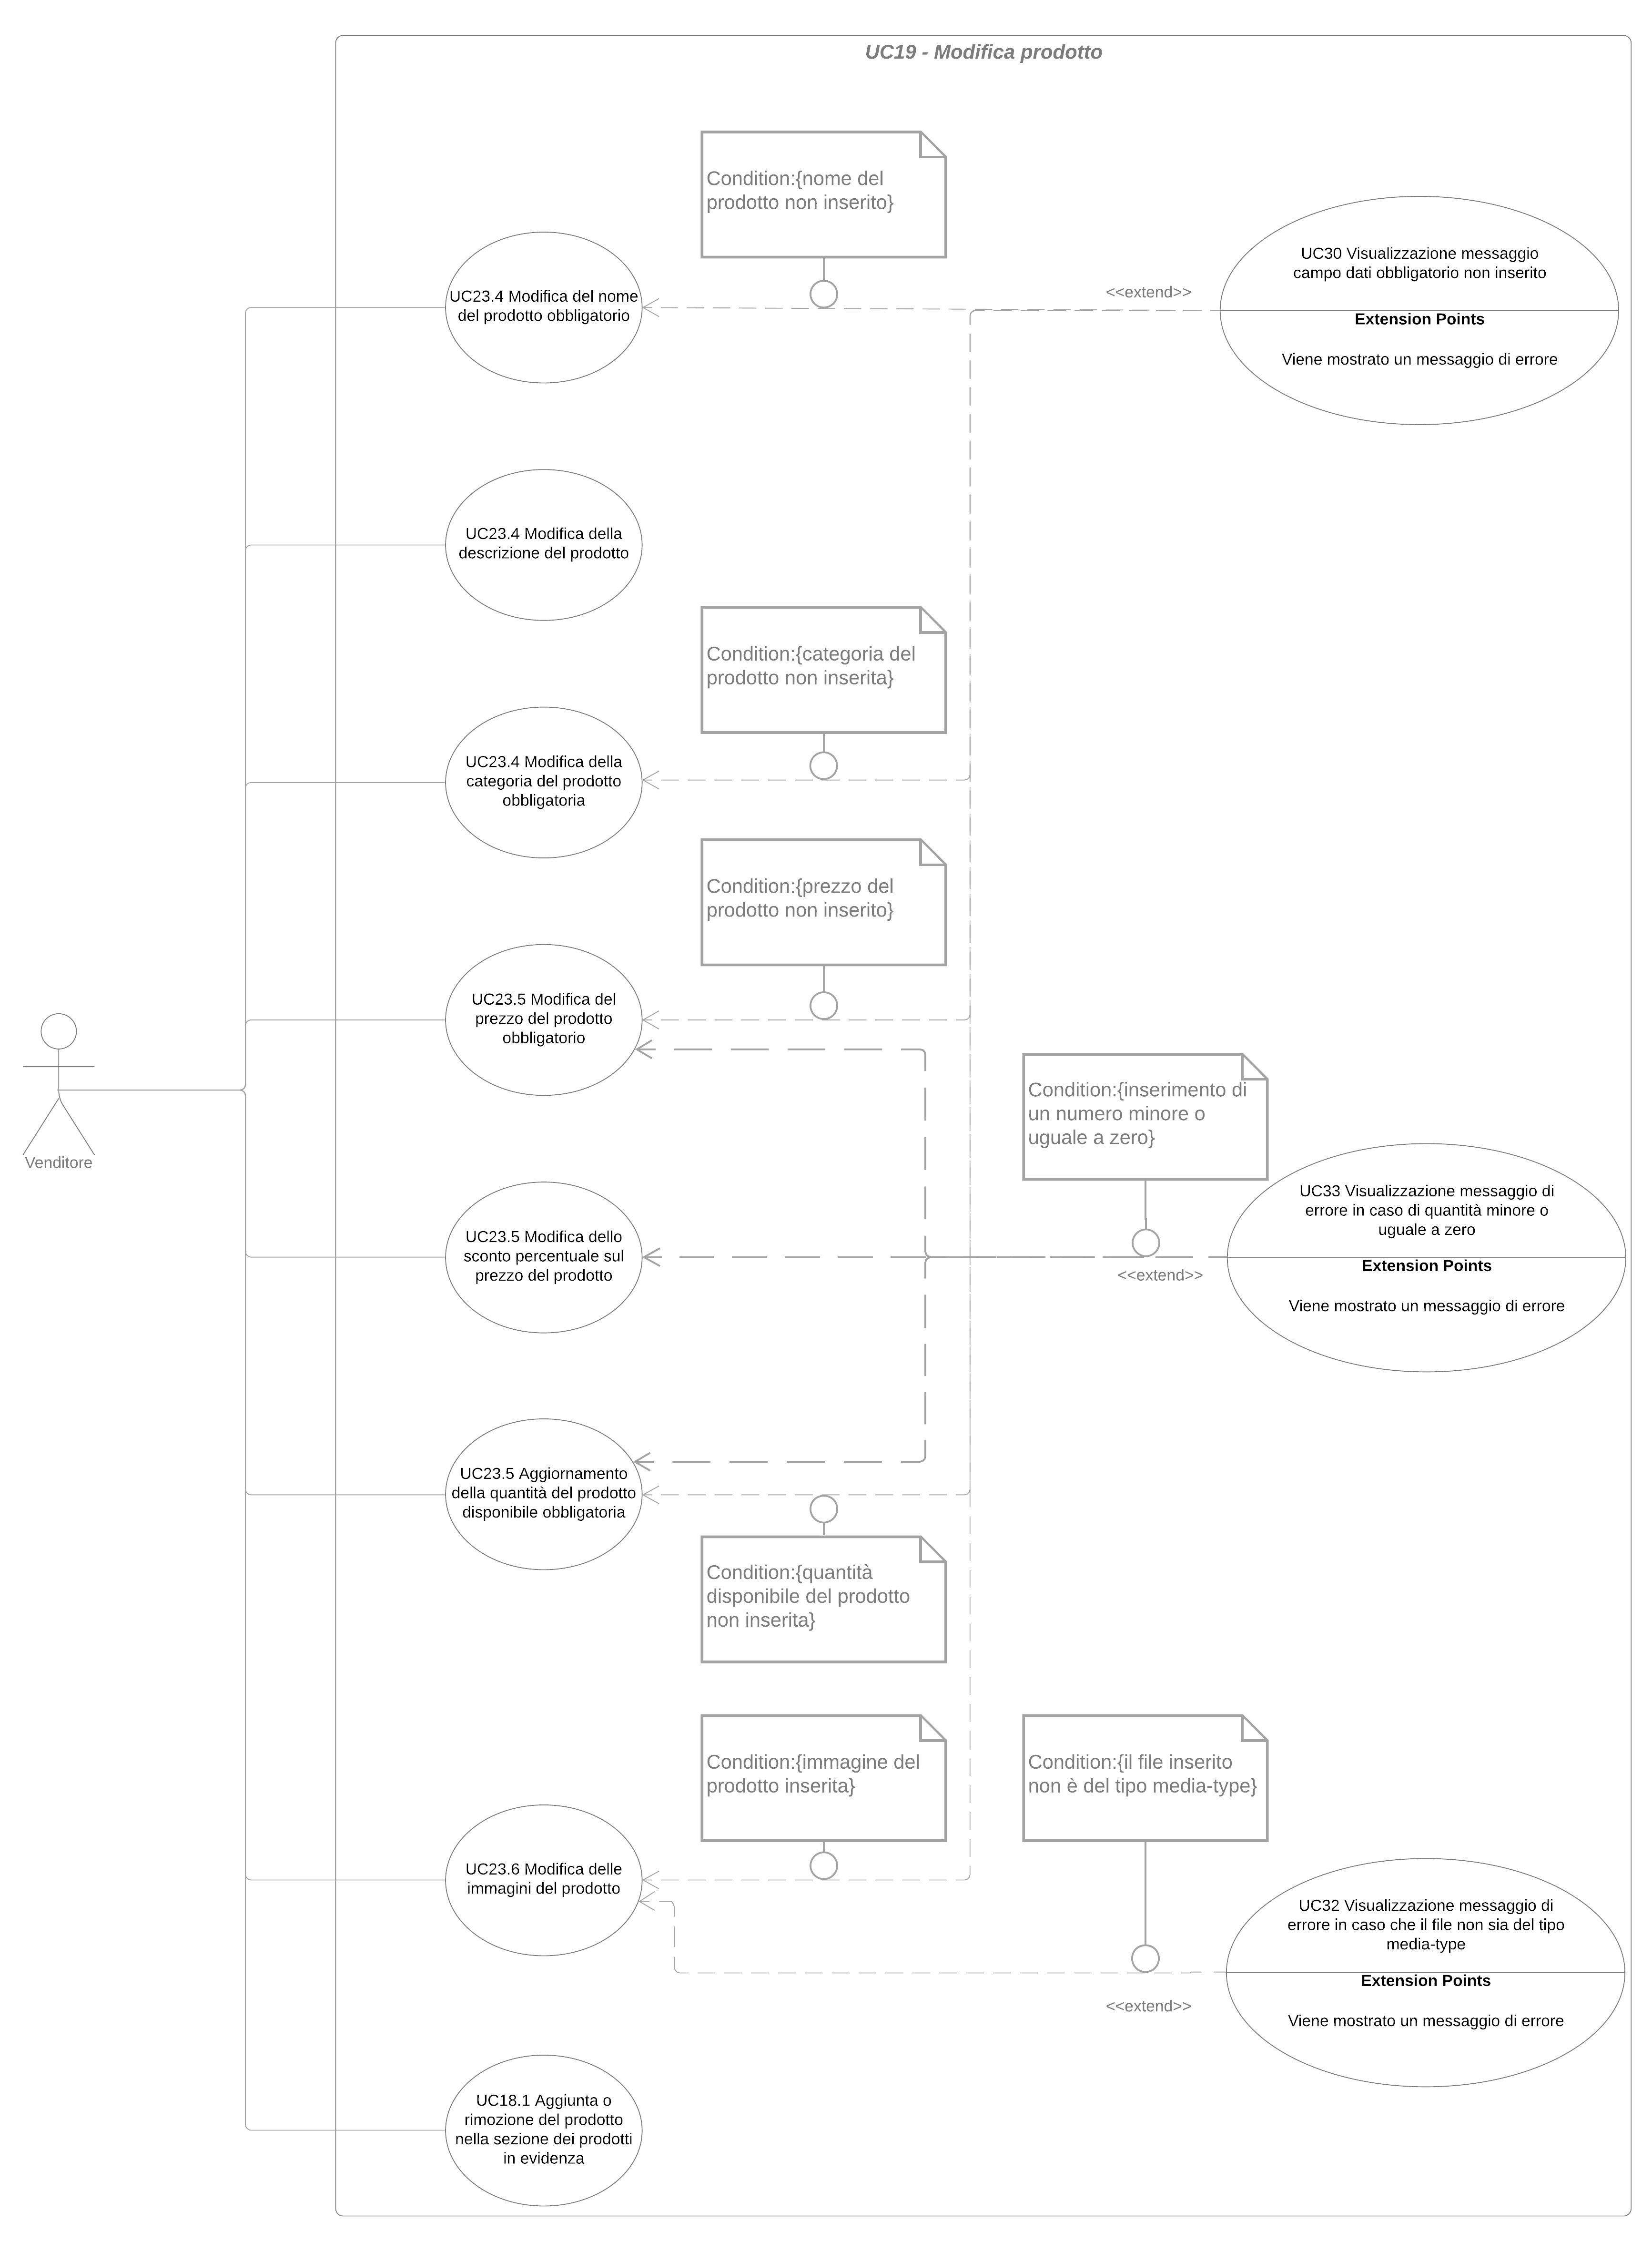
\includegraphics[scale=0.1]{Immagini/DiagrammiUC/UC19ModificaProdotto.png}
%     \caption{Diagramma di \actualUC: Modifica di un prodotto nella piattaforma da parte del venditore}
%     \label{fig:ModificaProdotto}
% \end{figure}

Il venditore modifica uno o più campi di un prodotto che è stato inserito nella piattaforma.
\begin{itemize}
    \item \textbf{Attori primari:} venditore;
    \item \textbf{Precondizione:} il venditore si trova nella PDP di un prodotto e clicca la funzionalità di modifica del prodotto selezionato;
    \item \textbf{Postcondizione:} il venditore ha modificato il prodotto con le modifiche compiute;
    \item \textbf{Scenario principale:} il venditore può compiere le seguenti azioni:
    \begin{itemize}
        \item (\actualUC.1) - Modifica del nome del prodotto;
        \item (\actualUC.2) - Modifica della descrizione del prodotto;
        \item (\actualUC.3) - Modifica delle categorie del prodotto;
        \item (\actualUC.4) - Modifica del prezzo del prodotto;
        \item (\actualUC.5) - Modifica dello sconto percentuale al prezzo del prodotto;
        \item (\actualUC.6) - Aggiunta di nuove foto del prodotto;
        \item (\actualUC.7) - Rimozione di foto del prodotto.
    \end{itemize}
    Il venditore conferma le modifiche compiute modificando in modo definitivo il prodotto selezionato;
    \item \textbf{Scenari alternativi:}
    \begin{enumerate}[label=\lett]
    	\item Il venditore non conferma le modifiche effettuate e perciò verranno scartate.
    \end{enumerate}
\end{itemize}

\resetSubUC
\subUC{Modifica del nome del prodotto}
Il venditore vuole modificare il nome del prodotto.
\begin{itemize}
    \item \textbf{Attori primari:} venditore;
    \item \textbf{Precondizione:} il venditore si trova nella schermata di modifica del prodotto;
    \item \textbf{Postcondizione:} il venditore ha modificato il nome del prodotto;
    \item \textbf{Scenario principale:} il venditore aggiorna il nome del prodotto selezionato;
    \item \textbf{Estensioni:}
    \begin{enumerate}[label=\lett]
    	\item Il venditore cancella il nome attuale del prodotto ed il campo dati risulta essere vuoto. In questo caso:
    	\begin{itemize}
    		\item (UC52) - Viene visualizzato il messaggio di errore campo dati obbligatorio non inserito;
    		\item Viene fornita al venditore la possibilità di inserire un nuovo nome al prodotto selezionato.
    	\end{itemize}
    \end{enumerate}
\end{itemize}

\subUC{Modifica della descrizione del prodotto}
Il venditore vuole modificare la descrizione del prodotto.
\begin{itemize}
    \item \textbf{Attori primari:} venditore;
    \item \textbf{Precondizione:} il venditore si trova nella schermata di modifica del prodotto;
    \item \textbf{Postcondizione:} il venditore ha modificato la descrizione del prodotto;
    \item \textbf{Scenario principale:} il venditore modifica la descrizione del prodotto selezionato;
    \item \textbf{Estensioni:}
    \begin{enumerate}[label=\lett]
    	\item Il venditore cancella la descrizione attuale del prodotto ed il campo dati risulta essere vuoto. In questo caso:
    	\begin{itemize}
    		\item (UC52) - Viene visualizzato il messaggio di errore campo dati obbligatorio non inserito;
    		\item Viene fornita al venditore la possibilità di inserire una nuova descrizione del prodotto selezionato.
    	\end{itemize}
    \end{enumerate}
\end{itemize}

\subUC{Modifica delle categorie del prodotto}
Il venditore modifica le categorie del prodotto.
\begin{itemize}
    \item \textbf{Attori primari:} venditore;
    \item \textbf{Precondizione:} il venditore si trova nella schermata di modifica del prodotto;
    \item \textbf{Postcondizione:} il venditore ha modificato le categorie del prodotto;
    \item \textbf{Scenario Principale:} il venditore modifica le categorie a cui fa parte il prodotto e può compiere le seguenti azioni:
    \begin{itemize}
        \item Aggiunta di una nuova categoria presa dalla lista di categorie disponibili;
        \item Rimozione di una categoria attualmente inserita.
    \end{itemize}
\end{itemize}

\subUC{Modifica del prezzo del prodotto}
Il venditore modifica il prezzo a cui vendere il prodotto.
\begin{itemize}
    \item \textbf{Attori primari:} venditore;
    \item \textbf{Precondizione:} il venditore si trova nella schermata di modifica del prodotto;
    \item \textbf{Postcondizione:} il venditore ha modificato il prezzo a cui vendere il prodotto;
    \item \textbf{Scenario principale:} il venditore modifica il prezzo a cui vendere il prodotto selezionato;
    \item \textbf{Estensioni:}
    \begin{enumerate}[label=\lett]
    	\item Il venditore cancella il prezzo attuale del prodotto ed il campo dati risulta essere vuoto. In questo caso:
    	\begin{itemize}
    		\item (UC52) - Viene visualizzato il messaggio di errore campo dati obbligatorio non inserito;
    		\item Viene fornita la possibilità al venditore di inserire un nuovo prezzo per il prodotto selezionato.
    	\end{itemize}
    	\item Il venditore inserisce un nuovo prezzo minore o uguale a 0. In questo caso:
    	\begin{itemize}
    		\item (UC59) - Verrà visualizzato il messaggio di errore in caso di prezzo minore o uguale a 0;
    		\item Viene fornita la possibilità al venditore di modificare il prezzo per il prodotto selezionato.
    	\end{itemize}
    \end{enumerate}
\end{itemize}

\subUC{Modifica dello sconto percentuale al prezzo del prodotto}
Il venditore modifica lo sconto percentuale da applicare al prezzo del prodotto.
\begin{itemize}
    \item \textbf{Attori primari:} venditore;
    \item \textbf{Precondizione:} il venditore si trova nella schermata di modifica del prodotto;
    \item \textbf{Postcondizione:} il venditore ha modificato lo sconto percentuale da applicare al prezzo del prodotto;
    \item \textbf{Scenario Principale:} il venditore modifica lo sconto percentuale da applicare al prezzo del prodotto selezionato;
    \item \textbf{Scenari alternativi:}
    \begin{enumerate}[label=\lett]
    	\item Nel caso in cui il venditore cancella lo sconto attuale senza inserirne uno di nuovo, non viene applicato alcuno sconto.
    \end{enumerate}
    \item \textbf{Estensioni:}
    \begin{enumerate}[label=\lett]
    	\item Il venditore inserisce uno sconto maggiore di 100\%. In questo caso:
		\begin{itemize}
			\item (UC62) - Viene visualizzato il messaggio di errore in caso di sconto maggiore di 100\%;
			\item Viene fornita al venditore la possibilità di modificare lo sconto da applicare al nuovo prodotto.
		\end{itemize}
		\item Il venditore inserisce uno sconto minore di 0\%. In questo caso:
		\begin{itemize}
			\item (UC61) - Viene mostrato un messaggio di errore che segnala lo sconto minore di 0\%;
			\item Viene fornita al venditore la possibilità di modificare lo sconto da applicare al nuovo prodotto.
		\end{itemize}
    \end{enumerate}
\end{itemize}

\subUC{Aggiunta di foto al prodotto}
Il venditore inserisce le foto relative al prodotto.
\begin{itemize}
    \item \textbf{Attori primari:} venditore;
    \item \textbf{Precondizione:} il venditore si trova nella schermata di modifica del prodotto;
    \item \textbf{Postcondizione:} il venditore ha inserito le foto relative al prodotto;
    \item \textbf{Scenario principale:} il venditore inserisce delle nuove foto relative al prodotto selezionato;
    \item \textbf{Estensioni:}
    \begin{enumerate}[label=\lett]
    	\item Il venditore seleziona un file che non è del tipo immagine. In questo caso:
		\begin{itemize}
			\item (UC58) - Viene visualizzato il messaggio di errore il quale segnala che il file selezionato non è del tipo immagine;
			\item Viene fornita la possibilità al venditore di cambiare i file selezionati per il nuovo prodotto.
		\end{itemize}
		\item Il venditore cerca di inserire più del numero massimo di foto consentite relative ad un prodotto. In questo caso:
		\begin{itemize}
			\item (UC63) - Viene visualizzato il messaggio di errore il quale segnala il tentativo di aggiunta di più del numero massimo di foto consentite relative ad un prodotto;
			\item Viene fornita la possibilità al venditore di rimuovere alcune foto selezionate per il nuovo prodotto da inserire.
		\end{itemize}
    \end{enumerate}
\end{itemize}

\subUC{Rimozione di foto dal prodotto}
Il venditore rimuove le foto relative al prodotto da aggiungere.
\begin{itemize}
    \item \textbf{Attori primari:} venditore;
    \item \textbf{Precondizione:} il venditore si trova nella schermata di modifica del prodotto;
    \item \textbf{Postcondizione:} il venditore ha rimosso le foto relative al prodotto;
    \item \textbf{Scenario principale:} il venditore rimuove le foto relative al prodotto attraverso i seguenti passi: 
    \begin{itemize}
        \item Seleziona la foto che vuole eliminare;
        \item Seleziona l'azione di eliminazione di quella specifica foto;
        \item Conferma la rimozione della foto selezionata.
    \end{itemize}
    \item \textbf{Estensioni:}
    \begin{enumerate}[label=\lett]
    	\item Il venditore cancella tutte le foto relative al prodotto. In questo caso:
    	\begin{itemize}
    		\item (UC52) - Viene visualizzato il messaggio di errore campo dati obbligatorio non inserito;
    		\item Viene impedita la conferma delle modifiche al prodotto.
    	\end{itemize}
    \end{enumerate}
\end{itemize}

\UC{Aggiunta prodotto alla sezione dei prodotti in evidenza}
Il venditore aggiunge un prodotto alla sezione dei prodotti in evidenza presente nella vista principale.
\begin{itemize}
    \item \textbf{Attori primari:} venditore;
    \item \textbf{Precondizione:} il venditore si trova nella PDP del prodotto ed il prodotto non è stato aggiunto alla sezione dei prodotti in evidenza;
    \item \textbf{Postcondizione:} il prodotto viene aggiunto alla sezione dei prodotti in evidenza;
    \item \textbf{Scenario principale:} il venditore aggiunge un prodotto alla sezione dei prodotti in evidenza tramite la funzionalità adeguata che lo segnerà come in evidenza.
\end{itemize}

\UC{Rimozione prodotto dalla sezione dei prodotti in evidenza}
Il venditore rimuove un prodotto dalla sezione dei prodotti in evidenza presente nella vista principale.
\begin{itemize}
    \item \textbf{Attori primari:} venditore;
    \item \textbf{Precondizione:} il venditore si trova nella PDP del prodotto ed il prodotto è stato aggiunto alla sezione dei prodotti in evidenza;
    \item \textbf{Postcondizione:} il prodotto viene rimosso dalla sezione dei prodotti in evidenza; 
    \item \textbf{Scenario principale:} il venditore rimuove un prodotto dalla sezione dei prodotti in evidenza tramite la funzionalità adeguata che lo segnerà come non in evidenza.
\end{itemize}

\UC{Eliminazione prodotto}
\begin{figure}[H]
    \centering
    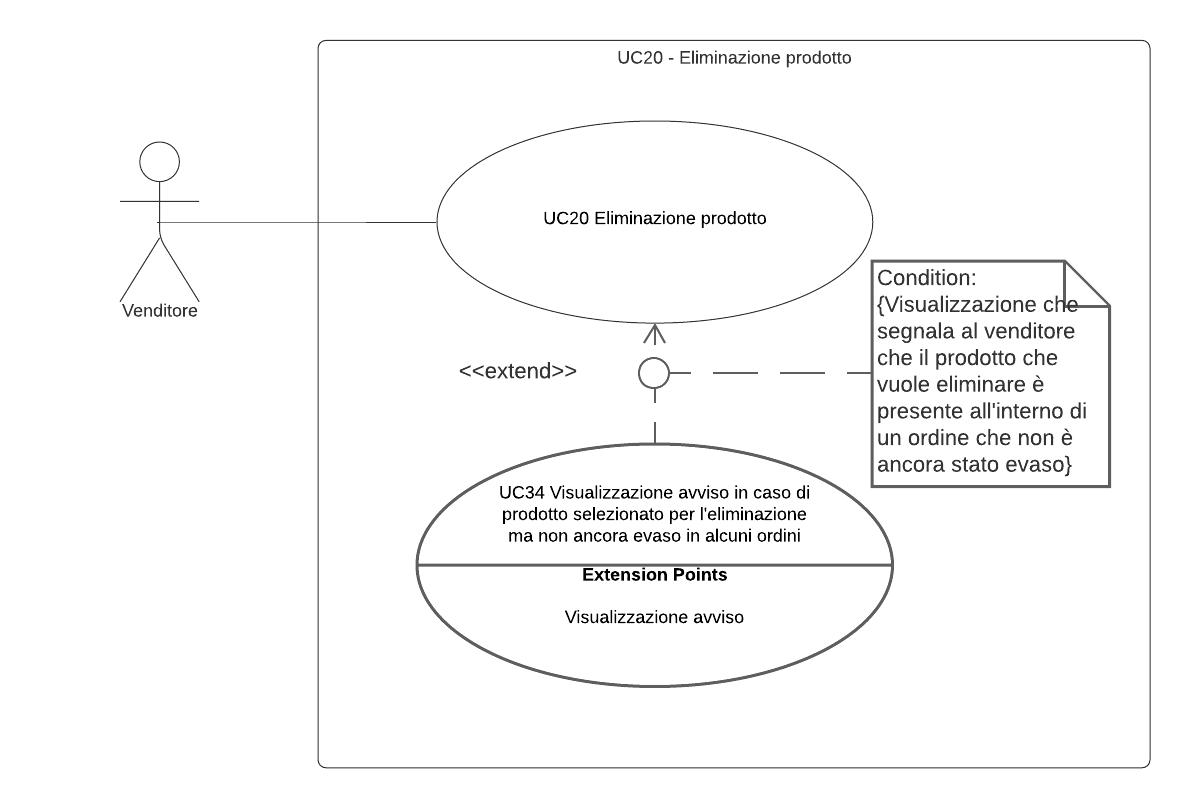
\includegraphics[width=\textwidth]{Immagini/DiagrammiUC/UC20EliminazioneProdotto}
    \caption{Diagramma di \actualUC: Eliminazione di un prodotto da parte del venditore} 
    \label{fig:EliminazioneProdotto}
\end{figure}

Il venditore vuole eliminare un prodotto precedentemente inserito.
\begin{itemize}
    \item \textbf{Attori primari:} venditore;
    \item \textbf{Precondizione:} il venditore si trova nella schermata della dashboard;
    \item \textbf{Postcondizione:} il venditore ha eliminato il prodotto selezionato;
    \item \textbf{Scenario Principale:} il venditore seleziona un prodotto dalla lista di quelli che ha inserito nella piattaforma, clicca sulla funzionalità per eliminarlo definitivamente e conferma l'eliminazione del prodotto selezionato. Di conseguenza:
    \begin{itemize}
    	\item Il prodotto viene rimosso da PDP, PLP, schermata principale, carrelli e dashboard;
    	\item Il prodotto rimane negli ordini già effettuati.
    \end{itemize}
	\item \textbf{Scenari alternativi:}
	\begin{enumerate}[label=\lett]
		\item Il venditore non conferma l'eliminazione del prodotto selezionato e di conseguenza questo rimarrà presente nella piattaforma.
	\end{enumerate}
\end{itemize}

\UC{Rifornimento prodotto}
Il venditore vuole rifornire un prodotto precedentemente inserito che sta per esaurire o è esaurito.
\begin{itemize}
    \item \textbf{Attori primari:} venditore;
    \item \textbf{Precondizione:} il venditore si trova nella schermata di amministrazione dei prodotti;
    \item \textbf{Postcondizione:} il venditore ha rifornito un prodotto;
    \item \textbf{Scenario principale:} il venditore seleziona un prodotto dalla lista di quelli che ha inserito nella piattaforma e preme sulla funzionalità per rifornirlo. Per completare il rifornimento deve svolgere i seguenti passi:
    \begin{itemize}
        \item Inserisce la quantità con cui rifornire il prodotto selezionato;
        \item Conferma il salvataggio della modifica.
    \end{itemize}
	\item \textbf{Scenari alternativi:}
	\begin{enumerate}[label=\lett]
		\item Il venditore inserisce la quantità con cui rifornire le scorte di un prodotto ma non conferma la modifica. In questo caso la quantità del prodotto non subisce alcuna modifica.
	\end{enumerate}
	\item \textbf{Estensioni:}
	\begin{enumerate}[label=\lett]
		\item Il venditore inserisce un valore inferiore a zero con cui rifornire le scorte di un determinato prodotto. In questo caso:
		\begin{itemize}
			\item (UC60) - Viene visualizzato un messaggio di errore in caso di quantità minore a zero;
			\item Viene fornita al venditore la possibilità di modificare il valore inserito per rifornire il prodotto.
		\end{itemize}
	\end{enumerate}
\end{itemize}

\UC{Ricerca dei prodotti del venditore} 
Il venditore può cercare i prodotti dalla propria PLP attraverso delle parole.
\begin{itemize}
	\item \textbf{Attori primari:} venditore;
	\item \textbf{Precondizione:} il venditore ha selezionato la funzionalità per la ricerca;
	\item \textbf{Postcondizione:} il venditore visualizza i prodotti che contengono nella descrizione o nel nome, almeno una delle parole per le quali si è svolta la ricerca;
	\item \textbf{Scenario principale:} il venditore ha selezionato la funzione prevista per la ricerca. Dopo aver inserito le parole per individuare il prodotto, conferma la ricerca e viene aggiornata la PLP che mostra tutti i prodotti che hanno almeno una delle parole indicate nella descrizione o nel nome;
	\item \textbf{Scenari alternativi:}
	\begin{enumerate}[label=\lett]
		\item Il venditore ha svolto una ricerca in modo tale che questa non dia alcun risultato. In questo caso la PLP del venditore viene aggiornata mostrando il messaggio nessun prodotto trovato.
	\end{enumerate}
\end{itemize}

%%%%%%%%%%%%%%%%%%%%%%%%%%%%%%%%%%%%%%%%%%%%%%%%%%%%%%%%%%%%%%%%%%%%%%%%%%%%%%%%%%%%%%%%%%%%%%%%%%%%%%%%%%%%%%%%%%%%%%%%%%%%%%%%%%%%%%%%%%%%%%%%%%%%%%%%%%%%%

\UC{Filtraggio prodotti della PLP del venditore}
\begin{figure}[H]
	\centering
	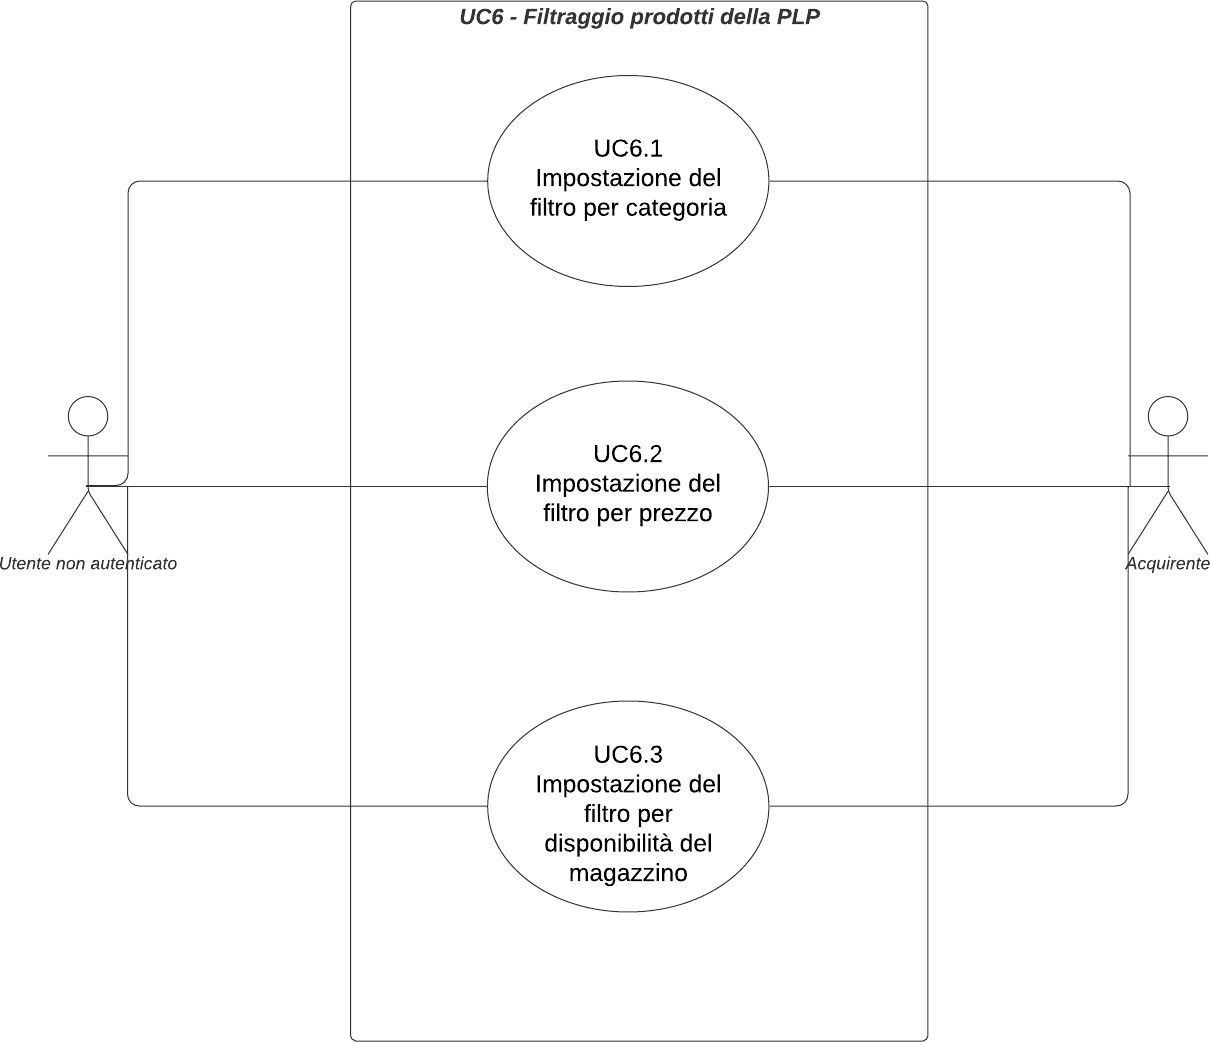
\includegraphics[scale=0.5]{Immagini/DiagrammiUC/UC6FiltraggioProdottiDellaPLP.png}
	\caption{Diagramma di \actualUC: Filtraggio dei prodotti della PLP} 
\end{figure}

Il venditore può filtrare i prodotti all'interno della PLP per categoria, prezzo, se è disponibile nel magazzino e se il prodotto è in evidenza o meno.
\begin{itemize}
	\item \textbf{Attori primari:} venditore;
	\item \textbf{Precondizione:} il venditore è nella PLP e ha impostato uno (o più) dei filtri disponibili per i quali cercare;
	\item \textbf{Postcondizione:} il venditore avrà a disposizione tutti i prodotti che soddisfano tutte le condizioni dei vari filtri impostati;
	\item \textbf{Scenario principale:} l'attore è nella PLP e ha impostato uno (o più) dei seguenti filtri:
	\begin{itemize}
		\item (\actualUC.1) - Impostazione del filtro per categoria;
		\item (\actualUC.2) - Impostazione del filtro per prezzo;
		\item (\actualUC.3) - Impostazione del filtro per disponibilità nel magazzino;
		\item (\actualUC.4) - Impostazione del filtro per prodotto in evidenza.
	\end{itemize}
	Di seguito la PLP verrà aggiornata con i prodotti che rispettano tutti i filtri applicati;
	\item \textbf{Scenari alternativi:}
	\begin{enumerate}[label=\lett]
		\item Il venditore ha impostato i filtri in modo tale che la ricerca con la loro combinazione non dia alcun risultato. In questo caso la schermata di riepilogo ordini viene aggiornata mostrando il messaggio nessun prodotto trovato.
	\end{enumerate}
\end{itemize}

\resetSubUC
\subUC{Filtro per categorie}
Il venditore può cercare i prodotti in base alla loro categoria, selezionando quelle di interesse tra tutte le categorie disponibili.
\begin{itemize}
	\item \textbf{Attori primari:} venditore;
	\item \textbf{Precondizione:} il venditore è nella PLP e ha selezionato una (o più) categorie tra quelle disponibili per quali filtrare;
	\item \textbf{Postcondizione:} il venditore visualizzerà nella PLP i prodotti che appartengono ad almeno una delle categorie selezionate;
	\item \textbf{Scenario principale:} il venditore è nella PLP e ha selezionato una (o più) categorie tra quelle disponibili per quali filtrare e di seguito verranno visualizzati i prodotti che appartengono ad almeno una delle categoria selezionate;
	\item \textbf{Scenari alternativi:}
	\begin{enumerate}[label=\lett]
		\item Se il venditore non imposta il seguente filtro, allora verranno visualizzati tutti i prodotti a prescindere della categoria.
	\end{enumerate}
\end{itemize}

\subUC{Filtro per prezzo}
Il venditore può cercare i prodotti in base al loro prezzo.
\begin{itemize}
	\item \textbf{Attori primari:} venditore;
	\item \textbf{Precondizione:} il venditore è nella PLP e ha selezionato uno tra gli intervalli di prezzo disponibili oppure ha inserito un intervallo personalizzato;
	\item \textbf{Postcondizione:} il venditore visualizzerà nella PLP i prodotti filtrati in base all'intervallo di prezzo selezionato;
	\item \textbf{Scenario principale:} il venditore seleziona l'intervallo di prezzo, oppure ne fornisce uno personalizzato per filtrare i prodotti, e verranno visualizzati i prodotti che entrano nell'intervallo di prezzo selezionato;
	\item \textbf{Scenari alternativi:}
	\begin{enumerate}[label=\lett]
		\item Se il venditore non imposta il seguente filtro, allora verranno visualizzati tutti i prodotti a prescindere dal prezzo.
	\end{enumerate}
\end{itemize}

\subUC{Filtro per disponibilità nel magazzino}
Il venditore può cercare i prodotti in base alla loro disponibilità in magazzino.
\begin{itemize}
	\item \textbf{Attori primari:} venditore;
	\item \textbf{Precondizione:} il venditore è nella PLP e ha attivato il filtro per disponibilità in magazzino;
	\item \textbf{Postcondizione:} il venditore visualizzerà nella PLP i prodotti che sono disponibili in magazzino;
	\item \textbf{Scenario principale:} il venditore ha attivato il filtro per disponibilità in magazzino e verranno visualizzati i prodotti che sono disponibili in magazzino;
	\item \textbf{Scenari alternativi:}
	\begin{enumerate}[label=\lett]
		\item Se il venditore non imposta il seguente filtro, allora verranno visualizzati tutti i prodotti a prescindere dalla loro disponibilità.
	\end{enumerate}
\end{itemize}

\subUC{Filtro per prodotto in evidenza}
Il venditore può cercare i prodotti in base alla loro caratteristica di trovarsi in evidenza o meno nella piattaforma.
\begin{itemize}
	\item \textbf{Attori primari:} venditore;
	\item \textbf{Precondizione:} il venditore è nella PLP e ha attivato il filtro per prodotto in evidenza;
	\item \textbf{Postcondizione:} il venditore visualizzerà nella PLP i prodotti che sono in evidenza;
	\item \textbf{Scenario principale:} il venditore ha attivato il filtro per prodotto in evidenza e verranno visualizzati i prodotti che sono in evidenza all'interno del sistema;
	\item \textbf{Scenari alternativi:}
	\begin{enumerate}[label=\lett]
		\item Se il venditore non imposta il seguente filtro, allora verranno visualizzati tutti i prodotti a prescindere dalla loro caratteristica di trovarsi in evidenza.
	\end{enumerate}
\end{itemize}

% Gestione categorie
\UC{Aggiunta nuova categoria}
Il venditore aggiunge una nuova categoria.
\begin{itemize}
    \item \textbf{Attori primari:} venditore;
    \item \textbf{Precondizione:} il venditore si trova nella schermata di amministrazione delle categorie e ha selezionato la funzionalità di aggiunta di una nuova categoria;
    \item \textbf{Postcondizione:} la categoria inserita è stata creata;
    \item \textbf{Scenario principale:}
    \begin{itemize}
    	\item Il venditore si trova nella schermata di amministrazione delle categorie;
    	\item Il venditore seleziona la funzionalità per aggiungere una nuova categoria di prodotti;
    	\item (UC) - Inserimento nome della nuova categoria;
    	\item Il venditore conferma la creazione della categoria di prodotti.
    \end{itemize} 
    \item \textbf{Scenari alternativi:}
    \begin{enumerate}[label=\lett]
    	\item Il venditore non conferma la creazione della categoria e di conseguenza questa non verrà aggiunta.
    \end{enumerate} 
\end{itemize}

\resetSubUC

\subUC{Inserimento nome della categoria}
Il venditore inserisce il nome della nuova categoria da aggiungere.
\begin{itemize}
    \item \textbf{Attori primari:} venditore;
    \item \textbf{Precondizione:} il venditore sta eseguendo l'azione di aggiunta di una nuova categoria;
    \item \textbf{Postcondizione:} il venditore ha inserito il nome della categoria;
    \item \textbf{Scenario principale:} il venditore compila il modulo per l'aggiunta della nuova categoria inserendo un nome;
    \item \textbf{Estensioni:}
    \begin{enumerate}[label=\lett]
    	\item Il venditore non inserisce alcun nome per la nuova categoria. In questo caso:
    	\begin{itemize}
    		\item (UC) - Verrà visualizzato il messaggio di errore campo dati obbligatorio non inserito;
    		\item Viene fornita al venditore la possibilità di modificare il nome della nuova categoria di prodotti.
    	\end{itemize}
    	\item Il venditore inserisce un nome per la nuova categoria che è già assegnato ad un'altra categoria. In questo caso:
    	\begin{itemize}
    		\item (UC) - Verrà visualizzato il messaggio di errore nome per la categoria già utilizzato;
    		\item Viene fornita al venditore la possibilità di modificare il nome della nuova categoria di prodotti.
    	\end{itemize}
    \end{enumerate}
\end{itemize}

\UC{Modifica di una categoria}
Il venditore modifica una categoria precedentemente inserita.
\begin{itemize}
    \item \textbf{Attori primari:} venditore;
    \item \textbf{Precondizione:} il venditore si trova nella schermata di amministrazione delle categorie e ha selezionato la funzionalità di modifica di una categoria precedentemente inserita;
    \item \textbf{Postcondizione:} la categoria selezionata viene modificata;
    \item \textbf{Scenario principale:}
    \begin{itemize}
    	\item Il venditore si trova nella schermata di amministrazione delle categorie;
    	\item Il venditore seleziona la funzionalità per modificare una categoria di prodotti;
    	\item (UC) - Modifica nome della categoria;
    	\item Il venditore conferma la modifica della categoria di prodotti.
    \end{itemize}
    \item \textbf{Scenari alternativi:} 
    \begin{enumerate}[label=\lett]
    	\item Il venditore non dà la conferma alle modifiche effettuate e di conseguenza la categoria non verrà modificata.
    \end{enumerate}
\end{itemize}

\resetSubUC

\subUC{Modifica nome della categoria}
Il venditore modifica il nome attuale di una categoria precedentemente inserita.
\begin{itemize}
    \item \textbf{Attori primari:} venditore;
    \item \textbf{Precondizione:} il venditore sta eseguendo l'azione di modifica di una categoria;
    \item \textbf{Postcondizione:} il venditore ha modificato il nome della categoria;
    \item \textbf{Scenario principale:} il venditore modifica la categoria inserendo un nuovo nome o modificando quello attuale;
    \item \textbf{Estensioni:}
    \begin{enumerate}[label=\lett]
    	\item Il venditore elimina il nome utilizzato in precedenza non inserendone uno nuovo. In questo caso:
    	\begin{itemize}
    		\item (UC) - Verrà visualizzato il messaggio di errore campo dati obbligatorio non inserito;
    		\item Viene fornita al venditore la possibilità di modificare il nome della nuova categoria di prodotti.
    	\end{itemize}
    	\item Il venditore modifica il nome della categoria con uno che è già assegnato ad un'altra categoria. In questo caso:
		\begin{itemize}
			\item (UC) - Verrà visualizzato il messaggio di errore nome per la categoria già utilizzato;
			\item Viene fornita al venditore la possibilità di modificare il nome della nuova categoria di prodotti.
		\end{itemize}
    \end{enumerate}
\end{itemize}

\UC{Eliminazione di una categoria}
Il venditore elimina una categoria precedentemente inserita.
\begin{itemize}
    \item \textbf{Attori primari:} venditore;
    \item \textbf{Precondizione:} il venditore si trova nella schermata di amministrazione delle categorie e ha selezionato la funzionalità di eliminazione di una categoria precedentemente inserita;
    \item \textbf{Postcondizione:} la categoria interessata viene eliminata;
    \item \textbf{Scenario principale:}
    \begin{itemize}
    	\item Il venditore si trova nella schermata di amministrazione delle categorie;
    	\item Il venditore seleziona la funzionalità per eliminare una categoria di prodotti;
    	\item Il venditore conferma la rimozione della categoria di prodotti con la conseguente eliminazione anche nei prodotti appartenenti alla categoria indicata.
    \end{itemize}
    \item \textbf{Scenari alternativi:}
    \begin{enumerate}[label=\lett]
    	\item Durante la visualizzazione del messaggio di conferma, il venditore non da il suo consenso per l'eliminazione e di conseguenza la categoria non verrà eliminata.
    \end{enumerate}
\end{itemize}

\UC{Ricerca categoria} 
Il venditore può cercare una categoria dalla propria schermata di amministrazione delle categorie.
\begin{itemize}
	\item \textbf{Attori primari:} venditore;
	\item \textbf{Precondizione:} il venditore ha selezionato la funzionalità per la ricerca;
	\item \textbf{Postcondizione:} il venditore visualizza le categorie che contengono nel nome almeno una delle parole per le quali si è svolta la ricerca;
	\item \textbf{Scenario principale:} il venditore ha selezionato la funzione prevista per la ricerca. Dopo aver inserito le parole per le quali individuare la categoria, avvia la ricerca e viene aggiornata la schermata di amministrazione delle categorie la quale visualizzerà tutte le categorie che hanno almeno una delle parole indicate nel nome;
	\item \textbf{Estensioni:}
	\begin{enumerate}[label=\lett]
		\item Il venditore ha svolto una ricerca che non ha prodotto alcun risultato. In questo caso:
		\begin{itemize}
			\item (UC) - Viene visualizzato il messaggio di ricerca senza alcun risultato.
		\end{itemize}
	\end{enumerate}
\end{itemize}


% Gestione ordini
\UC{Visualizzazione riepilogo ordini in gestione}
\label{visualizzazione-ordini-in-gestione}

Il venditore vuole vedere gli ordini chiusi o da gestire.
\begin{itemize}
    \item \textbf{Attori primari:} venditore;
    \item \textbf{Precondizione:} il venditore da qualsiasi schermata in cui si trovi vuole visualizzare gli ordini da gestire o già chiusi;
    \item \textbf{Postcondizione:} il venditore vede tutti gli ordini a suo carico in ordine cronologico decrescente;
    \item \textbf{Scenario principale:} il venditore vuole vedere tutti gli ordini a suo carico da gestire o già chiusi ed accede alla schermata di riepilogo ordini. Il venditore seleziona la funzionalità per accedere all'elenco degli ordini effettuati sulla piattaforma e visualizza l'elenco degli ordini ricevuti sulla piattaforma, dove è indicato per ogni ordine:
    \begin{itemize}
    	\item Il codice numerico dell'ordine;
    	\item Lo stato dell'ordine;
    	\item Il prezzo totale che è stato pagato;
    	\item L'indirizzo a cui è stato consegnato o verrà consegnato;
    	\item L'indirizzo e-mail dell'acquirente che ha effettuato l'ordine;
    	\item Una lista di tutti i prodotti acquistati in quell'ordine, dove per ogni prodotto verrà visualizzato:
    	\begin{itemize}
    		\item Nome del prodotto;
    		\item Quantità acquistata;
    		\item Prezzo totale del prodotto a cui è stato acquistato.
    	\end{itemize}
    \end{itemize}
	\item \textbf{Scenari alternativi:} 
	\begin{enumerate}[label=\lett]
		\item Il venditore non ha ancora ricevuto ordini, viene visualizzato il messaggio "Nessun ordine ricevuto" e viene data la possibilità al venditore di tornare alla propria dashboard.
	\end{enumerate}
\end{itemize}

\UC{Modifica stato ordine}
\label{modifica-stato-ordine}

Il venditore vuole modificare lo stato di un determinato ordine.
\begin{itemize}
	\item \textbf{Attori primari:} venditore;
	\item \textbf{Precondizione:} il venditore ha intenzione di modificare lo stato di un ordine a suo carico;
	\item \textbf{Postcondizione:} il venditore ha modificato lo stato di un ordine;
	\item \textbf{Scenario principale:}
	\begin{itemize}
		\item Il venditore seleziona un ordine dalla lista;
		\item Il venditore modifica lo stato dell'ordine.
	\end{itemize}
\end{itemize}

\UC{Ricerca di un ordine per codice}
\label{ricerca-codice-ordine-venditore}

Il venditore può cercare un ordine dalla propria schermata di riepilogo ordini.
\begin{itemize}
	\item \textbf{Attori primari:} venditore;
	\item \textbf{Precondizione:} il venditore ha selezionato la funzionalità per la ricerca e l'inserimento del codice per individuare un ordine;
	\item \textbf{Postcondizione:} il venditore visualizza l'ordine che corrisponde al codice per il quale si è svolta la ricerca;
	\item \textbf{Scenario principale:} il venditore ha selezionato la funzione prevista per la ricerca. Dopo aver inserito il codice per individuare l'ordine, conferma la ricerca e viene aggiornata la schermata di riepilogo ordini che mostra solamente l'ordine corrispondente al codice indicato;
	\item \textbf{Scenari alternativi:}
	\begin{enumerate}[label=\lett]
		\item Il venditore ha svolto una ricerca che non ha trovato coincidenze con nessun ordine ricevuto. In questo caso la schermata di riepilogo ordini viene aggiornata mostrando il messaggio nessun ordine trovato.
	\end{enumerate}
\end{itemize}

\UC{Ricerca di un ordine per cliente}
\label{ricerca-cliente-ordine-venditore}

Il venditore può cercare gli ordini in base al cliente che lo ha effettuato.
\begin{itemize}
	\item \textbf{Attori primari:} venditore;
	\item \textbf{Precondizione:} il venditore è nella schermata di riepilogo ordine ed ha inserito l'indirizzo e-mail di uno uno tra i clienti che hanno effettuato un ordine a suo carico;
	\item \textbf{Postcondizione:} il venditore visualizza la lista di ordini effettuati dal cliente per il quale si è svolta la ricerca;
	\item \textbf{Scenario principale:} il venditore ha selezionato la funzione prevista per la ricerca. Dopo aver inserito il cliente per individuare gli ordini, conferma la ricerca e viene aggiornata la schermata di riepilogo ordini che mostra solamente gli ordini effettuati dal cliente indicato;
	\item \textbf{Scenari alternativi:}
	\begin{enumerate}[label=\lett]
		\item Il venditore ha svolto una ricerca che non ha trovato coincidenze con nessun cliente. In questo caso la schermata di riepilogo ordini viene aggiornata mostrando il messaggio nessun ordine trovato.
	\end{enumerate}
\end{itemize}

\UC{Filtraggio ordini nella schermata di riepilogo ordini}
\label{filtro-ordini-venditore}

\begin{figure}[H]
    \centering
    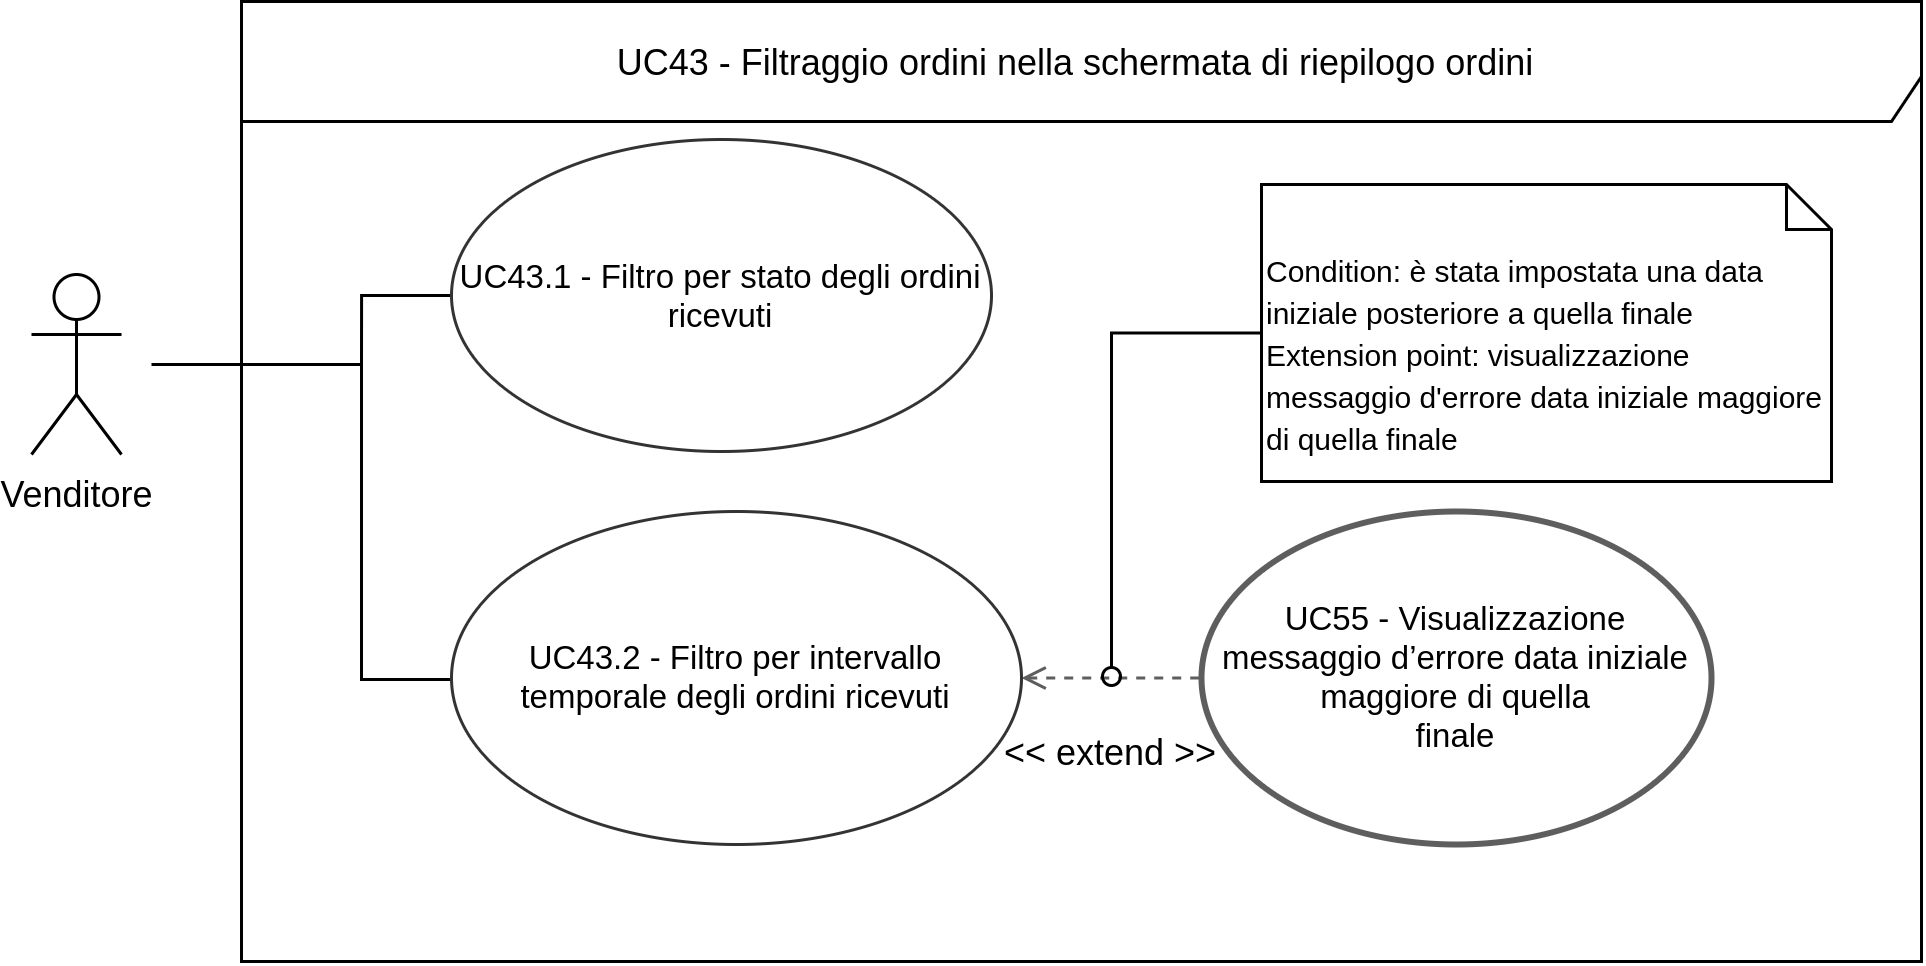
\includegraphics[width=\textwidth]{Immagini/DiagrammiUC/Venditore/FiltraggioOrdiniVenditore.png}
    \caption{Diagramma di \actualUC: Filtraggio ordini nella schermata di riepilogo ordini}
    \label{fig:filtro-ordini-venditore}
\end{figure}

Il venditore può filtrare gli ordini nella schermata di riepilogo ordini per lo stato dell'ordine secondo un intervallo temporale ed ordinarli in base alla loro data di accettazione.
\begin{itemize}
	\item \textbf{Attori primari:} venditore;
	\item \textbf{Precondizione:} il venditore è nella schermata di riepilogo ordini e ha impostato uno (o più) dei filtri disponibili per i quali cercare;
	\item \textbf{Postcondizione:} il venditore avrà a disposizione tutti gli ordini che soddisfano tutte le condizioni dei vari filtri impostati;
	\item \textbf{Scenario principale:} l'attore è nella schermata di riepilogo ordini e ha impostato uno (o più) dei seguenti filtri:
	\begin{itemize}
		\item (UC\ref{filtro-ordini-venditore.stato}) - Impostazione del filtro per stato degli ordini ricevuti;
		\item (UC\ref{filtro-ordini-venditore.temporale}) - Impostazione del filtro per intervallo temporale degli ordini ricevuti.
	\end{itemize}
	Di seguito la schermata di riepilogo ordini verrà aggiornata con gli ordini che rispettano tutti i filtri applicati;
	\item \textbf{Scenari alternativi:}
	\begin{enumerate}[label=\lett]
		\item Il venditore ha impostato i filtri in modo tale che la ricerca con la loro combinazione non dia alcun risultato. In questo caso la schermata di riepilogo ordini viene aggiornata mostrando il messaggio nessun ordine trovato.
	\end{enumerate}
\end{itemize}

\subUC{Filtro per stato degli ordini ricevuti}
\label{filtro-ordini-venditore.stato}

Il venditore può cercare gli ordini in base al loro stato, selezionando quelle di interesse tra tutti quelli disponibili.
\begin{itemize}
	\item \textbf{Attori primari:} venditore;
	\item \textbf{Precondizione:} il venditore è nella schermata di riepilogo ordini e ha selezionato uno (o più) stati tra quelli disponibili per quali filtrare;
	\item \textbf{Postcondizione:} il venditore visualizzerà nella schermata di riepilogo ordini gli ordini a suo carico che si trovano in uno degli stati selezionati;
	\item \textbf{Scenario principale:} il venditore è nella schermata di riepilogo ordini e ha selezionato uno (o più) stati tra quelli disponibili per quali filtrare e di seguito verranno visualizzati gli ordini che appartengono ad almeno uno degli stati selezionati;
	\item \textbf{Scenari alternativi:}
	\begin{enumerate}[label=\lett]
		\item Se il venditore non imposta il seguente filtro, allora verranno visualizzati tutti gli ordini ricevuti.
	\end{enumerate}
\end{itemize}

\subUC{Filtro per intervallo temporale degli ordini ricevuti}
\label{filtro-ordini-venditore.temporale}

\begin{figure}[H]
    \centering
    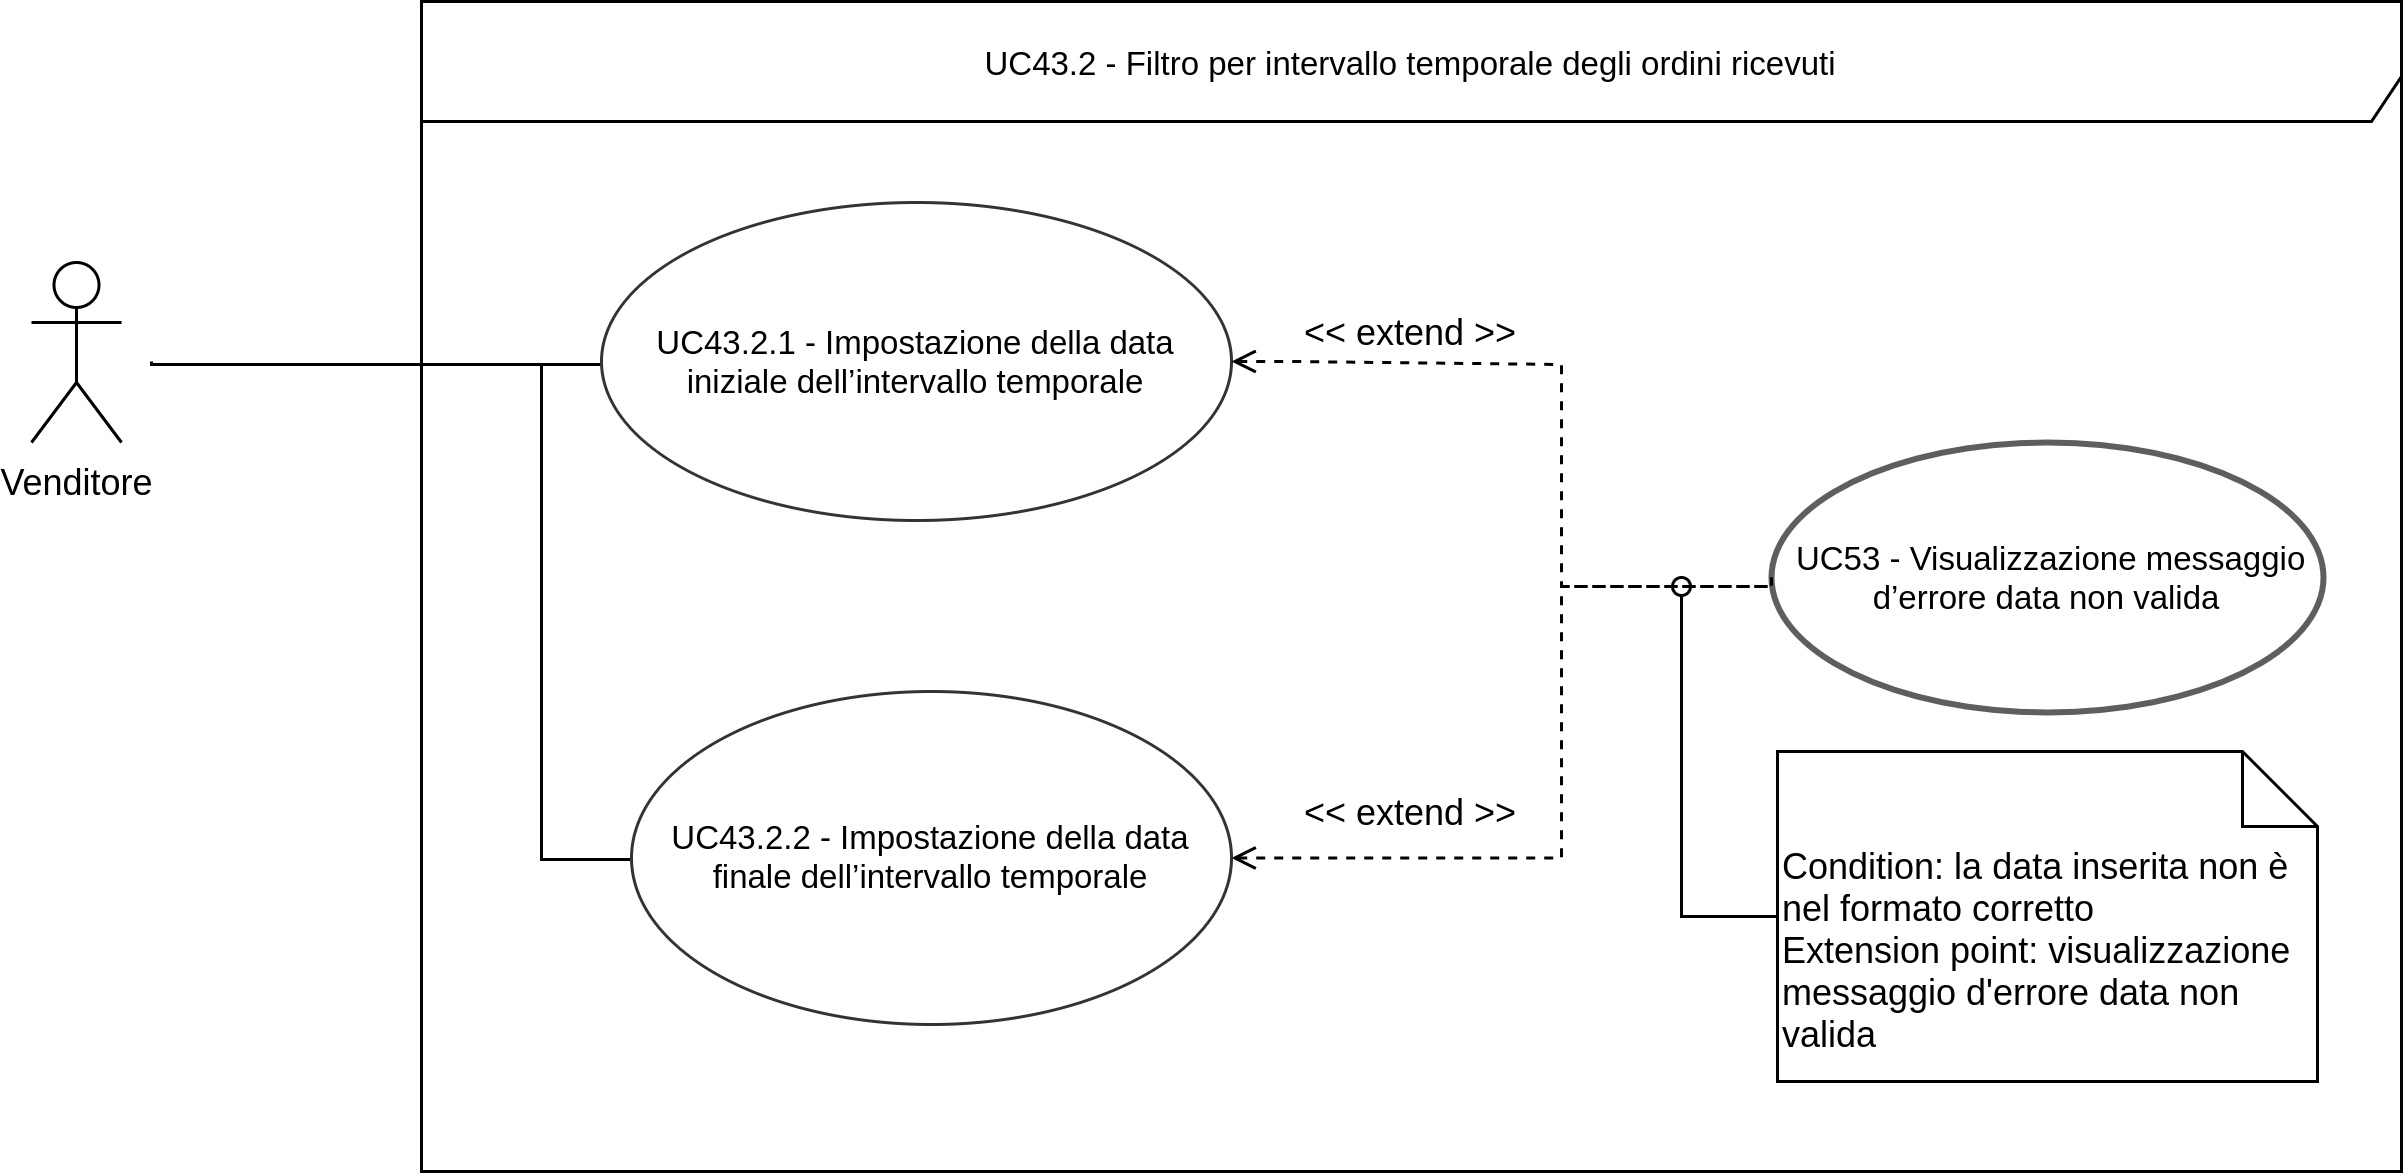
\includegraphics[width=\textwidth]{Immagini/DiagrammiUC/Venditore/FiltroIntervalloTemporaleVenditore.png}
    \caption{Diagramma di \actualSubUC: Filtro per intervallo temporale degli ordini ricevuti}
    \label{fig:filtro-ordini-venditore.temporale}
\end{figure}

Il venditore filtra temporalmente l'elenco degli ordini a suo carico sulla piattaforma.
\begin{itemize}
	\item \textbf{Attori primari:} venditore;
	\item \textbf{Precondizione:} il venditore si trova nella schermata di riepilogo ordini;
	\item \textbf{Postcondizione:} il venditore visualizza tutti gli ordini che sono stati fatti tra la data di inizio e quella di fine impostate;
	\item \textbf{Scenario principale:} il venditore si trova nella schermata di riepilogo ordini e vuole filtrare gli ordini a suo carico ricevuti durante un certo intervallo temporale. Per farlo dovrà:
	\begin{itemize}
		\item (UC\ref{filtro-ordini-venditore.temporale.data-iniziale}) - Impostare la data iniziale dell'intervallo temporale;
		\item (UC\ref{filtro-ordini-venditore.temporale.data-finale}) - Impostare la data finale dell'intervallo temporale.
	\end{itemize}
		\item \textbf{Scenari alternativi:}
	\begin{enumerate}[label=\lett]
		\item Se il venditore non imposta il seguente filtro, allora verranno visualizzati tutti gli ordini ricevuti dal più al meno recente.
	\end{enumerate}
	\item \textbf{Estensioni:}
	\begin{enumerate}[label=\lett]
		\item Il venditore inserisce una data iniziale maggiore di quella finale. In questo caso:
		\begin{itemize}
			\item (UC\ref{estensione:data-iniziale-maggiore-data-finale}) - Viene visualizzato il messaggio d'errore data iniziale maggiore di quella finale;
			\item Non verrà eseguita la ricerca.
		\end{itemize}
	\end{enumerate}
\end{itemize}

\subSubUC{Impostazione della data iniziale dell'intervallo temporale}
\label{filtro-ordini-venditore.temporale.data-iniziale}

Il venditore imposta la data iniziale dell'intervallo per il quale filtrare l'elenco degli ordini a suo carico ricevuti sulla piattaforma.
\begin{itemize}
	\item \textbf{Attori primari:} venditore;
	\item \textbf{Precondizione:} il venditore si trova nella schermata di riepilogo ordini;
	\item \textbf{Postcondizione:} il venditore ha impostato la data iniziale dell'intervallo per la quale filtrare l'elenco degli ordini ricevuti sulla piattaforma;
	\item \textbf{Scenario principale:} il venditore inserisce una data valida e minore o uguale a quella finale, come data iniziale dell'intervallo per la quale filtrare l'elenco degli ordini ricevuti;
	\item \textbf{Estensioni:}
	\begin{enumerate}[label=\lett]
		\item Il venditore inserisce una data iniziale non nel formato corretto. In questo caso:
		\begin{itemize}
			\item (UC\ref{estensione:data-non-valida}) - Viene visualizzato il messaggio d'errore data non valida;
			\item Non verrà eseguita la ricerca.
		\end{itemize} 
	\end{enumerate}
\end{itemize}

\subSubUC{Impostazione della data finale dell'intervallo temporale}
\label{filtro-ordini-venditore.temporale.data-finale}

Il venditore imposta la data finale dell'intervallo per il quale filtrare l'elenco degli ordini a suo carico ricevuti sulla piattaforma.
\begin{itemize}
	\item \textbf{Attori primari:} venditore;
	\item \textbf{Precondizione:} il venditore si trova nella schermata di riepilogo ordini;
	\item \textbf{Postcondizione:} il venditore ha impostato la data finale dell'intervallo per la quale filtrare l'elenco degli ordini ricevuti sulla piattaforma;
	\item \textbf{Scenario principale:} il venditore inserisce una data valida e maggiore o uguale di quella iniziale, come data finale dell'intervallo per la quale filtrare l'elenco degli ordini ricevuti;
	\item \textbf{Estensioni:}
	\begin{enumerate}[label=\lett]
		\item Il venditore inserisce una data finale non nel formato corretto. In questo caso:
		\begin{itemize}
			\item (UC\ref{estensione:data-non-valida}) - Viene visualizzato il messaggio d'errore data non valida;
			\item Non verrà eseguita la ricerca.
		\end{itemize}
	\end{enumerate}
\end{itemize}

% Estensioni
% Estensioni campi dati
\UC{Visualizzazione messaggio di errore caratteri non alfabetici non permessi}
Visualizzazione messaggio di errore che segnala all'attore l'inserimento di caratteri non alfabetici.
\begin{itemize}
    \item \textbf{Attori primari:} acquirente;
    \item \textbf{Precondizione:} l'attore ha inserito dei caratteri non alfabetici;
    \item \textbf{Postcondizione:} all'attore verrà mostrato un messaggio il quale lo informa della presenza di carattere non alfabetici, dove non è permessa la loro presenza;
    \item \textbf{Scenario principale:} l'attore ha inserito dei caratteri non alfabetici dove non è permessa la loro presenza e verrà avvisato della presenza di caratteri non alfabetici.
\end{itemize}

% Estensioni email
\UC{Visualizzazione messaggio di errore in caso di registrazione con un'email già utilizzata nella piattaforma}
Visualizzazione messaggio di errore che segnala all'attore il tentativo di registrazione con un'email già utilizzata nella piattaforma.
\begin{itemize}
    \item \textbf{Attori primari:} utente non autenticato;
    \item \textbf{Precondizione:} l'utente non autenticato sta cercando di registrarsi con un'email già utilizzata nella piattaforma;
    \item \textbf{Postcondizione:} all'attore viene mostrato un messaggio il quale indica l'impossibilità di registrarsi con un'email già utilizzata nella piattaforma;
    \item \textbf{Scenario principale:} l'attore sta cercando di registrarsi con un'email già utilizzata nella piattaforma e viene avvisato dell'impossibilità di registrarsi con un'email già utilizzata nella piattaforma.
\end{itemize}

\UC{Visualizzazione messaggio di errore in caso di cambio email con una già utilizzata nella piattaforma}
Visualizzazione messaggio di errore che segnala all'attore il tentativo di cambio dell'email attuale con un'email già utilizzata nella piattaforma.
\begin{itemize}
    \item \textbf{Attori primari:} acquirente o venditore;
    \item \textbf{Precondizione:} l'attore sta cercando di cambiare la propria email con una già utilizzata nella piattaforma;
    \item \textbf{Postcondizione:} all'attore viene mostrato un messaggio il quale indica l'impossibilità di cambiare la propria email attuale con un'email già utilizzata nella piattaforma;
    \item \textbf{Scenario principale:} l'attore sta cercando di cambiare la propria email attuale con un'email già utilizzata nella piattaforma e viene avvisato dell'impossibilità di cambiare la propria email con una già utilizzata nella piattaforma.
\end{itemize}

\UC{Visualizzazione messaggio di errore in caso di email non registrata}
Visualizzazione messaggio di errore che segnala all'attore il tentativo di accesso alla piattaforma con una email non registrata.
\begin{itemize}
    \item \textbf{Attori primari:} utente non autenticato;
    \item \textbf{Precondizione:} l'utente non autenticato ha inserito un'email non registrata nella piattaforma;
    \item \textbf{Postcondizione:} all'utente non autenticato viene mostrato un messaggio il quale indica l'impossibilità di inserire un'email non registrata nella piattaforma;
    \item \textbf{Scenario principale:} l'utente non autenticato ha inserito un'email non registrata nella piattaforma e viene informato dell'impossibilità di inserire un'email non registrata nella piattaforma.
\end{itemize}

\UC{Visualizzazione messaggio di errore in caso di credenziali non presenti nella piattaforma}
Visualizzazione messaggio di errore che segnala all'utente il tentativo di accesso alla piattaforma attraverso delle credenziali non presenti nella piattaforma.
\begin{itemize}
    \item \textbf{Attori primari:} utente non autenticato;
    \item \textbf{Precondizione:} l'utente non autenticato tenta di accedere alla piattaforma attraverso delle credenziali non presenti in essa;
    \item \textbf{Postcondizione:} all'utente non autenticato viene mostrato un messaggio il quale lo avvisa dell'utilizzo di credenziali non presenti nella piattaforma;
    \item \textbf{Scenario principale:} l'utente non autenticato tenta di accedere alla piattaforma attraverso delle credenziali non presenti in essa e viene informato dell'utilizzo di credenziali non presenti nella piattaforma.
\end{itemize}

\UC{Visualizzazione messaggio di errore in caso di email non valida}
Visualizzazione messaggio di errore che segnala all'utente che l'email inserita non rispetta il formato di un indirizzo email.
\begin{itemize}
    \item \textbf{Attori primari:} utente autenticato o utente non autenticato;
    \item \textbf{Precondizione:} l'attore ha inserito un'email nel formato sbagliato;
    \item \textbf{Postcondizione:} all'utente non autenticato viene mostrato un messaggio il quale lo avvisa dell'inserimento di un'email in un formato errato;
    \item \textbf{Scenario principale:} l'attore ha inserito un'email nel formato sbagliato e viene informato dell'inserimento di un'email nel formato sbagliato.
\end{itemize}

% Estensioni password
\UC{Visualizzazione messaggio di errore in caso di password troppo debole}
Visualizzazione messaggio di errore che segnala all'utente l'inserimento di una password troppo debole che non rispetta le condizioni minime per essere accettabile.
\begin{itemize}
    \item \textbf{Attori primari:} utente autenticato o utente non autenticato;
    \item \textbf{Precondizione:} l'attore ha inserito una password troppo debole;
    \item \textbf{Postcondizione:} all'attore viene mostrato un messaggio il quale lo avvisa dell'inserimento di una password che non rispetta le condizioni minime per essere accettabile;
    \item \textbf{Scenario principale:} l'attore ha inserito una password troppo debole che non rispetta le condizioni minime per essere accettabile e viene informato del non rispetto delle condizioni minime.
\end{itemize}

\UC{Visualizzazione messaggio di errore in caso di password e password di conferma diverse}
Visualizzazione messaggio di errore che segnala all'utente la non corrispondenza della password e della password di conferma inserite.
\begin{itemize}
    \item \textbf{Attori primari:} utente autenticato o utente non autenticato;
    \item \textbf{Precondizione:} l'attore inserisce una password di conferma che non corrisponde a quella inserita come password da registrare;
    \item \textbf{Postcondizione:} all'attore viene mostrato un messaggio il quale lo avvisa della non corrispondenza tra la password e la password di conferma;
    \item \textbf{Scenario principale:} l'attore inserisce una password di conferma che non corrisponde a quella inserita come password da registrare e viene informato della non corrispondenza.
\end{itemize}

\UC{Visualizzazione messaggio campo dati obbligatorio non inserito}
Visualizzazione messaggio che segnala all'utente il mancato riempimento di un campo dati obbligatorio.
\begin{itemize}
    \item \textbf{Attori primari:} utente autenticato o utente non autenticato;
    \item \textbf{Precondizione:} l'attore non ha inserito, oppure ha inserito solo caratteri vuoti come spazi o tab, in un campo dati obbligatorio;
    \item \textbf{Postcondizione:} all'attore viene mostrato un messaggio che lo avvisa del mancato riempimento di quel campo dati obbligatorio;
    \item \textbf{Scenario principale:} l'attore non ha inserito, oppure ha inserito solo caratteri vuoti come spazi o tab, in un campo dati obbligatorio e viene informato del mancato riempimento di esso.
\end{itemize}

% Estensioni ordini
\UC{Visualizzazione messaggio d'errore data non valida}
Visualizzazione messaggio di errore che segnala all'attore l'inserimento di una data non valida.
\begin{itemize}
    \item \textbf{Attori primari:} utente autenticato o utente non autenticato;
    \item \textbf{Precondizione:} l'attore ha inserito una data non nel formato corretto;
    \item \textbf{Postcondizione:} all'attore verrà mostrato un messaggio il quale lo informa dell'inserimento di una data non valida;
    \item \textbf{Scenario principale:} l'attore ha inserito una data non nel formato giorno/mese/anno e viene informato del formato non valido della data.
\end{itemize}

\UC{Visualizzazione messaggio d'errore data iniziale maggiore di quella finale}
Visualizzazione messaggio di errore che segnala all'attore l'inserimento di una data iniziale maggiore di quella finale.
\begin{itemize}
    \item \textbf{Attori primari:} utente autenticato o utente non autenticato;
    \item \textbf{Precondizione:} l'attore ha inserito una data iniziale maggiore di quella finale;
    \item \textbf{Postcondizione:} all'attore verrà mostrato un messaggio il quale lo informa dell'inserimento di una data iniziale maggiore di quella finale;
    \item \textbf{Scenario principale:} l'attore ha inserito una data iniziale maggiore di quella finale e viene informato dell'impossibilità di inserire una data iniziale maggiore di quella finale.
\end{itemize}

% Estensioni carrello
\begin{comment}
\UC{Visualizzazione messaggio di errore prodotto non disponibile}
L'acquirente o l'utente non autenticato richiede un prodotto che non è disponibile.
\begin{itemize}
    \item \textbf{Attori primari:} acquirente o utente non autenticato;
    \item \textbf{Precondizione:} l'attore richiede di aggiungere al carrello un prodotto non disponibile;
    \item \textbf{Postcondizione:} viene impedita l'aggiunta al carrello e segnalata la causa.
    \item \textbf{Scenario principale:}
        \begin{itemize}
            \item L'utente richiede di aggiungere al carrello un prodotto non disponibile;
            \item Viene scartata la modifica, il carrello rimane invariato;
            \item Viene visualizzato un visualizzato un errore che indica la non disponibilità del prodotto.
        \end{itemize}
\end{itemize}
\end{comment}

% Estensioni info personali
\UC{Visualizzazione messaggio di errore nel caso in cui il file selezionato non sia del tipo immagine}
Visualizzazione messaggio di errore che segnala al venditore che il file inserito non è di tipo immagine.
\begin{itemize}
    \item \textbf{Attori primari:} venditore;
    \item \textbf{Precondizione:} il venditore inserisce un file di tipo non immagine;
    \item \textbf{Postcondizione:} all'attore viene mostrato un messaggio il quale lo avvisa che si possono selezionare solo file di tipo immagine;
    \item \textbf{Scenario principale:} il venditore inserisce un file di tipo non immagine e viene informato del tipo errato del file.
\end{itemize}

% Estensioni prodotto
\UC{Visualizzazione messaggio di errore in caso di prezzo minore o uguale a zero}
Visualizzazione messaggio di errore il quale segnala al venditore che il prezzo del prodotto inserito è minore o uguale a zero.
\begin{itemize}
    \item \textbf{Attori primari:} venditore;
    \item \textbf{Precondizione:} il venditore inserisce un prezzo minore o uguale a zero;
    \item \textbf{Postcondizione:} al venditore viene mostrato un messaggio il quale lo avvisa che il prezzo del prodotto inserito è minore o uguale a zero;
    \item \textbf{Scenario principale:} il venditore inserisce un prezzo minore o uguale a zero e viene informato dell'inserimento di un prezzo minore o uguale a zero.
\end{itemize}

\UC{Visualizzazione messaggio di errore in caso di quantità minore o uguale a zero}
Visualizzazione messaggio di errore che segnala al venditore che la quantità del prodotto inserita è minore o uguale a zero.
\begin{itemize}
    \item \textbf{Attori primari:} venditore;
    \item \textbf{Precondizione:} il venditore inserisce una quantità del prodotto minore o uguale a zero;
    \item \textbf{Postcondizione:} al venditore viene mostrato un messaggio il quale lo avvisa che la quantità del prodotto inserita è minore o uguale a zero;
    \item \textbf{Scenario principale:} il venditore inserisce una quantità del prodotto minore o uguale a zero e viene informato dell'inserimento di una quantità minore o uguale a zero.
\end{itemize}

\UC{Visualizzazione messaggio di errore in caso di sconto minore di zero}
Visualizzazione messaggio di errore il quale segnala al venditore che lo sconto inserito è minore di zero.
\begin{itemize}
    \item \textbf{Attori primari:} venditore;
    \item \textbf{Precondizione:} il venditore inserisce uno sconto minore di zero;
    \item \textbf{Postcondizione:} al venditore viene mostrato un messaggio il quale lo avvisa che lo sconto appena inserito è minore di zero;
    \item \textbf{Scenario principale:} il venditore inserisce uno sconto minore di zero e viene informato dell'inserimento di uno sconto minore di zero.
\end{itemize}

\UC{Visualizzazione messaggio di errore in caso di sconto maggiore di 100\%}
Visualizzazione messaggio di errore il quale segnala al venditore che lo sconto inserito è maggiore di 100\%.
\begin{itemize}
    \item \textbf{Attori primari:} venditore;
    \item \textbf{Precondizione:} il venditore inserisce uno sconto maggiore di 100\%;
    \item \textbf{Postcondizione:} al venditore viene mostrato un messaggio il quale lo avvisa che lo sconto appena inserito è maggiore di 100\%;
    \item \textbf{Scenario principale:} il venditore inserisce uno sconto maggiore di 100\% e viene informato dell'inserimento di uno sconto maggiore di 100\%.
\end{itemize}

\UC{Visualizzazione messaggio di errore tentivo di aggiunta di più di quattro foto relative ad un prodotto}
Visualizzazione messaggio di errore il quale segnala al venditore il tentativo di aggiunta di una nuova foto relativa ad un prodotto, quando si è già raggiunto il limite massimo di quattro.
\begin{itemize}
    \item \textbf{Attori primari:} venditore;
    \item \textbf{Precondizione:} il venditore cerca di aggiungere una nuova foto relativa ad un prodotto, anche quando si è già raggiunto il limite massimo di quattro;
    \item \textbf{Postcondizione:} al venditore viene mostrato un messaggio il quale lo avvisa che non possono essere inserite più di 4 quattro foto per prodotto;
    \item \textbf{Scenario principale:} il venditore cerca di aggiungere una nuova foto relativa ad un prodotto, anche quando si è già raggiunto il limite massimo di quattro e viene informato del superamento del limite di quattro foto per prodotto.
\end{itemize}

\UC{Visualizzazione messaggio di errore nessuna foto inserita}
Visualizzazione messaggio di errore il quale segnala al venditore che non è stata inserita alcuna foto relativa al prodotto.
\begin{itemize}
    \item \textbf{Attori primari:} venditore;
    \item \textbf{Precondizione:} il venditore non inserisce alcuna foto relativa ad un prodotto;
    \item \textbf{Postcondizione:} al venditore viene mostrato un messaggio il quale lo avvisa che bisogna inserire almeno una foto relativa ad un prodotto;
    \item \textbf{Scenario principale:} il venditore non inserisce alcuna foto relativa ad un prodotto e viene informato del mancato inserimento di almeno una foto relativa ad un prodotto.
\end{itemize}

% Estensioni Categoria
\UC{Visualizzazione messaggio nome per la categoria già utilizzato}
Visualizzazione messaggio di errore il quale segnala al venditore che sta cercando di assegnare ad una categoria un nome già utilizzato da un'altra.
\begin{itemize}
    \item \textbf{Attori primari:} venditore;
    \item \textbf{Precondizione:} il venditore vuole assegnare ad una categoria un nome già utilizzato da un'altra categoria;
    \item \textbf{Postcondizione:} al venditore viene mostrato un messaggio il quale lo avvisa che il nome che sta cercando di assegnare ad una categoria è già in uso;
    \item \textbf{Scenario principale:} il venditore vuole assegnare ad una categoria un nome già utilizzato da un'altra categoria e viene informato dell'impossibilità di assegnare ad una categoria un nome già utilizzato da un'altra categoria.
\end{itemize}

% Estensioni dashboard

\UC{Visualizzazione messaggio di ricerca senza alcun risultato}
Nel caso in cui la ricerca del prodotto non dia risultati verrà visualizzato un opportuno messaggio.
\begin{itemize}
	\item \textbf{Attori primari:} acquirente o utente non autenticato;
	\item \textbf{Precondizione:} l'attore ha svolto una ricerca di un prodotto che non ha dato alcun risultato;
	\item \textbf{Postcondizione:} all'attore verrà mostrato un messaggio il quale lo informa che la ricerca appena effettuata non ha prodotto alcun risultato;
	\item \textbf{Scenario principale:} l'attore effettua una ricerca che non ha prodotto alcun risultato e viene informato del mancato risultato della ricerca appena effettuata.
\end{itemize}

\UC{Visualizzazione messaggio nessun ordine effettuato nell'arco temporale impostato}
Visualizzazione di un messaggio il quale segnala all'acquirente che non è stato effettuato alcun ordine nell'arco temporale impostato.
\begin{itemize}
    \item \textbf{Attori primari:} acquirente;
    \item \textbf{Precondizione:} l'acquirente ha inserito un intervallo temporale nel quale non è stato effettuato alcun ordine;
    \item \textbf{Postcondizione:} all'acquirente verrà mostrato un messaggio il quale lo informa della non effettuazione di alcun ordine nell'arco temporale impostato;
    \item \textbf{Scenario principale:} l'acquirente ha inserito un intervallo temporale nel quale non è stato effettuato alcun ordine e viene informato della non effettuazione di alcun ordine nell'arco temporale impostato.
\end{itemize}

\UC{Visualizzazione messaggio in caso di prodotto selezionato per l'eliminazione ma non ancora evaso in alcuni ordini}
Visualizzazione messaggio il quale segnala al venditore che il prodotto che vuole eliminare è presente all'interno di un ordine che non è ancora stato evaso.
\begin{itemize}
    \item \textbf{Attori primari:} venditore;
    \item \textbf{Precondizione:} il venditore sta cercando di eliminare un prodotto all'interno in un ordine che non è stato ancora evaso;
    \item \textbf{Postcondizione:} al venditore viene mostrato un messaggio il quale lo informa che il prodotto non può essere eliminato perché è presente in un ordine che non è stato ancora evaso;
    \item \textbf{Scenario principale:} il venditore sta cercando di eliminare un prodotto presente in un ordine che non è stato ancora evaso, viene quindi informato che per questo motivo non è possibile procedere con l'eliminazione.
\end{itemize}

% Estensioni carta per il pagamento
\UC{Visualizzazione messaggio d'errore numero della carta non valido}
Nel caso in cui venga inserito un numero di una carta non valido, verrà segnalato attraverso un messaggio di errore opportuno.
\begin{itemize}
	\item \textbf{Attori primari:} acquirente;
	\item \textbf{Precondizione:} l'acquirente ha inserito un numero di una carta non valido;
	\item \textbf{Postcondizione:} all'acquirente verrà mostrato un messaggio il quale lo informa della non validità del numero della carta;
	\item \textbf{Scenario principale:} l'attore non ha inserito esattamente 16 numeri compresi tra 0 e 9 come numero della carta e verrà avvisato della non validità del numero della carta.
\end{itemize}

\UC{Visualizzazione messaggio d'errore CVV della carta non valido}
Nel caso in cui venga inserito un CVV di una carta non valido, verrà segnalato attraverso un messaggio di errore opportuno.
\begin{itemize}
	\item \textbf{Attori primari:} acquirente;
	\item \textbf{Precondizione:} l'acquirente ha inserito un CVV di una carta non valido;
	\item \textbf{Postcondizione:} all'acquirente verrà mostrato un messaggio il quale lo informa della non validità del CVV della carta;
	\item \textbf{Scenario principale:} l'attore non ha inserito esattamente 3 numeri compresi tra 0 e 9 come CVV della carta e verrà avvisato della non validità del CVV della carta.
\end{itemize}

\UC{Visualizzazione messaggio d'errore data di scandenza non valida}
Nel caso in cui venga inserita una data di scadenza di una carta non valida, verrà segnalato attraverso un messaggio di errore opportuno.
\begin{itemize}
	\item \textbf{Attori primari:} acquirente;
	\item \textbf{Precondizione:} l'acquirente ha inserito una data di scadenza di una carta non valida;
	\item \textbf{Postcondizione:} all'acquirente verrà mostrato un messaggio il quale lo informa della non validità della data di scadenza della carta;
	\item \textbf{Scenario principale:} l'attore non ha inserito una data di scadenza valida nel seguente formato "mese/anno", dove l'anno sarà composto solo dalle ultime due cifre dell'anno di scadenza, e verrà avvisato della non validità della data di scadenza.
\end{itemize}

% Estensioni indirizzo di consegna
\UC{Visualizzazione messaggio d'errore CAP non valido}
Nel caso in cui venga inserito un CAP per un indirizzo di consegna non valido, verrà segnalato attraverso un messaggio di errore opportuno.
\begin{itemize}
	\item \textbf{Attori primari:} acquirente;
	\item \textbf{Precondizione:} l'acquirente ha inserito un CAP per un indirizzo di consegna non valido;
	\item \textbf{Postcondizione:} all'acquirente verrà mostrato un messaggio il quale lo informa della non validità del CAP inserito;
	\item \textbf{Scenario principale:} l'attore non ha inserito un CAP composto da esattamente 5 numeri compresi tra 0 e 9 e verrà avvisato della non validità del CAP.
\end{itemize}

% Estensioni stripe
\UC{Visualizzazione messaggio d'errore pagamento non andato a buon fine}
Nel caso in cui avvenga un errore durante lo svolgimento del pagamento da parte di stripe, questo verrà visualizzato all'acquirente.
\begin{itemize}
	\item \textbf{Attori primari:} acquirente;
	\item \textbf{Attori secondari:} stripe;
	\item \textbf{Precondizione:} stripe sta svolgendo il pagamento dell'acquirente e si verifica un errore;
	\item \textbf{Postcondizione:} all'acquirente verrà mostrato un messaggio il quale lo informa della non riuscita del pagamento con il relativo messaggio;
	\item \textbf{Scenario principale:} stripe sta svolgendo il pagamento dell'acquirente, si verifica un errore e questo verrà visualizzato all'acquirente informandolo dell'errore specifico.
\end{itemize}


% \setcounter{secnumdepth}{9}

\newpage
\section{Requisiti}

\subsection{Introduzione}
In questa parte, vengono riportati i requisiti del progetto, classificati per tipologia. Ciascun requisito possiede un codice identificativo, il cui formalismo viene riportato all'interno del documento \NdPv{1.0.0}.

\subsection{Requisiti funzionali} \label{ReqFunz}
\rowcolors{2}{white}{celeste} 
\renewcommand{\arraystretch}{1.5}

\addcontentsline{lot}{table}{Requisiti funzionali}

\begin{longtable}{c C{9.5cm} C{2.5cm}} 

	\rowcolor{darkblue}
	\textcolor{white}{\textbf{Codice Requisito}}&
	\textcolor{white}{\textbf{Descrizione}}&
    \textcolor{white}{\textbf{Fonte}} \\
    
    % Acquirente
    \rfun{O}{\ref{registrazione}} & L'utente non autenticato che non dispone di credenziali può registrarsi e accedere come acquirente alla piattaforma. & UC\ref{registrazione} \\ 

\rfun{O}{\ref{registrazione.modulo.nome}} & L'utente non autenticato inserisce il nome con il quale vuole registrarsi. & UC\ref{registrazione.modulo.nome} \\

\rfun{O}{\ref{registrazione.modulo.cognome}} & L'utente non autenticato inserisce il cognome con il quale vuole registrarsi. & UC\ref{registrazione.modulo.cognome} \\

\rfun{O}{\ref{registrazione.modulo.email}} & L'utente non autenticato inserisce l'indirizzo e-mail con il quale vuole registrarsi. & UC\ref{registrazione.modulo.email} \\

\rfun{O}{\ref{registrazione.modulo.password}} & L'utente non autenticato inserisce la password con la quale vuole registrarsi. & UC\ref{registrazione.modulo.password} \\

\rfun{O}{\ref{registrazione.modulo.conferma-password}} & L'utente non autenticato inserisce la conferma della password con la quale vuole registrarsi. & UC\ref{registrazione.modulo.conferma-password} \\

\rfun{O}{\ref{autenticazione-venditore}} & L'utente non autenticato che dispone di credenziali venditore può accedere alla piattaforma usando l'e-mail e la password & UC\ref{autenticazione-venditore} \\

\rfun{O}{\ref{autenticazione-acquirente}} & L'utente non autenticato che dispone di credenziali acquirente può accedere nella piattaforma usando l'e-mail e la password & UC\ref{autenticazione-acquirente} \\

\rfun{O}{\ref{password-dimenticata}} & L'utente non autenticato che dispone di credenziali acquirente o venditore e si è dimenticato la propria password, potrà cambiarla. & UC\ref{password-dimenticata} \\

\rfun{O}{} & L'utente non autenticato potrà accedere alla schermata per l'autenticazione da qualsiasi schermata della piattaforma. & Interna \\

\rfun{O}{\ref{logout}} & L'utente autenticato potrà scollegarsi dalla piattaforma da qualsiasi schermata della piattaforma. & UC\ref{logout} \\


    \rfun{O}{\ref{ricerca-prodotti-acquirente}} & L'utente non autenticato e l'acquirente può cercare i prodotti attraverso delle parole dalla schermata principale, oppure dalla PLP. & UC\ref{ricerca-prodotti-acquirente} \\

\rfun{O}{\ref{filtro-prodotti-acquirente}} & L'utente non autenticato o l'acquirente può filtrare i prodotti all'interno della \glo{PLP}. & UC\ref{filtro-prodotti-acquirente} \\

\rfun{O}{\ref{filtro-prodotti-acquirente.categoria}} & L'utente non autenticato o l'acquirente può cercare i prodotti in base alla loro categoria, selezionando quelle di interesse tra tutte le categorie disponibili. & UC\ref{filtro-prodotti-acquirente.categoria} \\

\rfun{O}{\ref{filtro-prodotti-acquirente.prezzo}} & L'utente non autenticato o l'acquirente può cercare i prodotti in base al loro prezzo. & UC\ref{filtro-prodotti-acquirente.prezzo} \\

\rfun{O}{\ref{filtro-prodotti-acquirente.magazzino}} & L'utente non autenticato o l'acquirente può cercare i prodotti in base alla loro disponibilità in magazzino. & UC\ref{filtro-prodotti-acquirente.magazzino} \\


    \rfun{O}{} & L'utente non autenticato o l'acquirente visualizzerà i prodotti nella PLP ordinati alfabeticamente come ordinamento predefinito & Capitolato \\

\rfun{O}{} & L'utente non autenticato o l'acquirente, nella PLP, visualizzerà una lista di tutti i prodotti corrispondenti alla ricerca, dove per ogni prodotto sarà visualizzabile: il nome del prodotto, la prima immagine disponibile di esso, il suo prezzo per unità e se è disponibile in magazzino o no & Capitolato \\

\rfun{O}{} & I prodotti nella PLP non disponibili devono essere distinti da quelli che lo sono. & Capitolato \\

\rfun{O}{\ref{ordinamento-alfabetico}} & L'utente non autenticato o l'acquirente può ordinare i prodotti risultanti dalla ricerca effettuata in precedenza per ordine alfabetico. & UC\ref{ordinamento-alfabetico} \\

\rfun{O}{\ref{ordinamento-prezzo-crescente}} & L'utente non autenticato o l'acquirente può ordinare i prodotti risultanti dalla ricerca effettuata in precedenza per prezzo crescente. & UC\ref{ordinamento-prezzo-crescente} \\

\rfun{O}{\ref{ordinamento-prezzo-decrescente}} & L'utente non autenticato o l'acquirente può ordinare i prodotti risultanti dalla ricerca effettuata in precedenza per prezzo decrescente. & UC\ref{ordinamento-prezzo-decrescente} \\

\rfun{O}{\ref{aggiunta-carrello-plp}} & L'utente non autenticato o l'acquirente può aggiungere al carrello un'unità di un prodotto direttamente dalla PLP, avendo anche la possibilità di modificare in precedenza la quantità da aggiungere. & UC\ref{aggiunta-carrello-plp} \\

% \rfun{O}{\ref{}} &  & UC\ref{} \\


    \rfun{O}{} & L'utente non autenticato o l'acquirente può accedere alla \glo{PDP} di un prodotto in evidenza dalla schermata principale. & Interna \\

\rfun{O}{} & L'utente non autenticato o l'acquirente può accedere alla PDP di un prodotto acquistato dalla schermata di riepilogo ordine. & Interna \\

\rfun{O}{} & L'utente non autenticato o l'acquirente può accedere alla PDP di un prodotto che è stato aggiunto al carrello. & \glo{Capitolato} \\

\rfun{O}{} & L'utente non autenticato o l'acquirente può accedere alla PDP di un prodotto dalla PLP. & Capitolato \\

\rfun{O}{} & L'utente non autenticato o l'acquirente dalla PDP potrà visualizzare: nome del prodotto, la sua descrizione, le categorie alle quali appartiene, foto relative ad esso, il prezzo e relativi sconti. & Interna \\

\rfun{O}{\ref{aggiunta-carrello-pdp}} & L'utente non autenticato o l'acquirente può aggiungere al carrello un'unità di un prodotto direttamente dalla PDP, avendo anche la possibilità di modificare in precedenza la quantità da aggiungere. & UC\ref{aggiunta-carrello-pdp} \\

\rfun{O}{\ref{modifica-quantita-da-aggiungere-al-carrello}} & L'acquirente o l'utente non autenticato modifica la quantità del prodotto che vuole aggiungere nel carrello. & UC\ref{modifica-quantita-da-aggiungere-al-carrello} \\

% \rfun{O}{\ref{}} &  & UC\ref{} \\


    \rfun{O}{} & L'utente non autenticato o l'acquirente può accedere alla schermata del carrello da qualsiasi altra schermata della piattaforma. & Capitolato \\

\rfun{O}{\ref{visualizzazione-carrello}} & L'utente non autenticato o l'acquirente potrà visualizzare il proprio carrello, dove potrà visualizzare il prezzo totale e l'elenco dei prodotti. & UC\ref{visualizzazione-carrello} \\

\rfun{O}{\ref{visualizzazione-carrello}} & L'utente non autenticato o l'acquirente potrà visualizzare il proprio carrello dove per ogni prodotto inserito sarà indicato: il nome del prodotto, la quantità inserita, il prezzo del prodotto in base alla quantità inserita e agli sconti disponibili e la prima foto disponibile del prodotto. & UC\ref{visualizzazione-carrello} \\

\rfun{O}{\ref{eliminazione-prodotto-dal-carrello}} & L'utente non autenticato o l'acquirente può eliminare un prodotto che ha inserito nel carrello. & UC\ref{eliminazione-prodotto-dal-carrello} \\

\rfun{O}{\ref{modifica-quantita-nel-carrello}} & L'utente non autenticato o l'acquirente modifica la quantità di un prodotto precedentemente inserito nel carrello. & UC\ref{modifica-quantita-nel-carrello} \\

% \rfun{O}{\ref{}} &  & UC\ref{} \\


    \rfun{O}{\ref{checkout}} & L'acquirente può procedere al checkout per effettuare l'ordine con i prodotti inseriti nel carrello. & UC\ref{checkout} \\

\rfun{O}{\ref{checkout.indirizzo}} & L'acquirente seleziona l'indirizzo della consegna, ovvero dove verrà recapitato l'acquisto, tra gli indirizzi di consegna precedentemente inseriti. & UC\ref{checkout.indirizzo} \\

\rfun{O}{\ref{checkout.pagamento}} & L'acquirente procede al pagamento attraverso il servizio fornito dal gestore dei pagamenti. & UC\ref{checkout.pagamento} \\

\rfun{O}{\ref{inserimento-indirizzo-consegna}} & L'acquirente può aggiungere un nuovo indirizzo di consegna. & UC\ref{inserimento-indirizzo-consegna} \\

\rfun{O}{\ref{inserimento-indirizzo-consegna.modulo.nazione}} & L'acquirente può selezionare la nazione dell'indirizzo di consegna. & UC\ref{inserimento-indirizzo-consegna.modulo.nazione} \\

\rfun{O}{\ref{inserimento-indirizzo-consegna.modulo.comune}} & L'acquirente può inserire il comune dell'indirizzo di consegna. & UC\ref{inserimento-indirizzo-consegna.modulo.comune} \\

\rfun{O}{\ref{inserimento-indirizzo-consegna.modulo.via}} & L'acquirente può inserire la via dell'indirizzo di consegna, includendo anche il numero civico e l'eventuale interno. & UC\ref{inserimento-indirizzo-consegna.modulo.via} \\

\rfun{O}{\ref{inserimento-indirizzo-consegna.modulo.cap}} & L'acquirente può inserire il CAP dell'indirizzo di consegna. & UC\ref{inserimento-indirizzo-consegna.modulo.cap} \\

\rfun{O}{\ref{modifica-indirizzo-consegna}} & L'acquirente può modificare un indirizzo di consegna precedentemente inserito. & UC\ref{modifica-indirizzo-consegna} \\

\rfun{O}{\ref{modifica-indirizzo-consegna.nazione}} & L'acquirente può modificare la nazione dell'indirizzo di consegna. & UC\ref{modifica-indirizzo-consegna.nazione} \\

\rfun{O}{\ref{modifica-indirizzo-consegna.comune}} & L'acquirente può modificare il comune dell'indirizzo di consegna. & UC\ref{modifica-indirizzo-consegna.comune} \\

\rfun{O}{\ref{modifica-indirizzo-consegna.via}} & L'acquirente può modificare la via dell'indirizzo di consegna. & UC\ref{modifica-indirizzo-consegna.via} \\

\rfun{O}{\ref{modifica-indirizzo-consegna.cap}} & L'acquirente può modificare il CAP dell'indirizzo di consegna. & UC\ref{modifica-indirizzo-consegna.cap} \\

\rfun{O}{\ref{eliminazione-indirizzo-consegna}} & L'acquirente può eliminare un indirizzo di consegna precedentemente inserito. & UC\ref{eliminazione-indirizzo-consegna} \\

% \rfun{O}{\ref{}} &  & UC\ref{} \\


    \rfun{O}{} & L'acquirente può accedere alla schermata con tutti gli ordini effettuati da qualsiasi altra schermata della piattaforma. & Interna \\

\rfun{O}{\ref{visualizzazione-ordini-effettuati}} & L'acquirente può visualizzare l'elenco degli ordini effettuati sulla piattaforma. Per ognuno di questi potrà visualizzare: il codice numerico dell'ordine, lo stato dell'ordine, il prezzo totale che è stato pagato, l'indirizzo a cui è stato consegnato o verrà consegnato e una lista di tutti i prodotti acquistati.& UC\ref{visualizzazione-ordini-effettuati} \\

\rfun{O}{\ref{visualizzazione-ordini-effettuati}} & L'acquirente può visualizzare i prodotti che sono stati acquistati in un ordine effettuato. Per ognuno di questi verrà visualizzato: il nome del prodotto, la quantità acquistata e il prezzo totale a cui è stato acquistato. & UC\ref{visualizzazione-ordini-effettuati} \\

\rfun{O}{\ref{ricerca-codice-ordine-acquirente}} & L'acquirente può cercare un ordine sapendo il suo codice numerico. & UC\ref{ricerca-codice-ordine-acquirente} \\

\rfun{O}{\ref{filtro-temporale-ordini-acquirente}} & L'acquirente può filtrare temporalmente l'elenco degli ordini effettuati sulla piattaforma. & UC\ref{filtro-temporale-ordini-acquirente} \\

\rfun{O}{\ref{filtro-temporale-ordini-acquirente.data-iniziale}} & L'acquirente può impostare la data iniziale dell'intervallo per il quale filtrare l'elenco degli ordini effettuati sulla piattaforma. & UC\ref{filtro-temporale-ordini-acquirente.data-iniziale} \\

\rfun{O}{\ref{filtro-temporale-ordini-acquirente.data-finale}} & L'acquirente impostare la data finale dell'intervallo per il quale filtrare l'elenco degli ordini effettuati sulla piattaforma. & UC\ref{filtro-temporale-ordini-acquirente.data-finale} \\

% \rfun{O}{\ref{}} &  & UC\ref{} \\


    \rfun{O}{} & L'acquirente può accedere alla schermata con le proprie informazioni da qualsiasi altra schermata della piattaforma. & Interna \\

\rfun{O}{} & L'acquirente, nella propria schermata personale, potrà visualizzare: il nome ed il cognome che ha inserito e l'indirizzo e-mail collegato al proprio account. & Interna \\

\rfun{O}{\ref{modifica-informazioni-acquirente}} & L'acquirente può modificare le sue informazioni personali. & UC\ref{modifica-informazioni-acquirente} \\

\rfun{O}{\ref{modifica-informazioni-acquirente.nome}} & L'acquirente può modificare il nome con il quale si è registrato. & UC\ref{modifica-informazioni-acquirente.nome} \\

\rfun{O}{\ref{modifica-informazioni-acquirente.cognome}} & L'acquirente può modificare il cognome con il quale si è registrato. & UC\ref{modifica-informazioni-acquirente.cognome} \\

\rfun{O}{\ref{modifica-informazioni-acquirente.email}} & L'acquirente può modificare l'indirizzo e-mail con il quale si autenticherà. & UC\ref{modifica-informazioni-acquirente.email} \\

\rfun{O}{\ref{modifica-informazioni-acquirente.password}} & L'acquirente può modificare la password con la quale si autenticherà. & UC\ref{modifica-informazioni-acquirente.password} \\

\rfun{O}{\ref{eliminazione-account-acquirente}} & L'acquirente può eliminare il proprio account. & UC\ref{eliminazione-account-acquirente} \\

% \rfun{O}{\ref{}} &  & UC\ref{} \\

% \rfun{O}{\ref{}} &  & UC\ref{} \\

% \rfun{O}{\ref{}} &  & UC\ref{} \\

% \rfun{O}{\ref{}} &  & UC\ref{} \\

% \rfun{O}{\ref{}} &  & UC\ref{} \\

% \rfun{O}{\ref{}} &  & UC\ref{} \\

% \rfun{O}{\ref{}} &  & UC\ref{} \\

% \rfun{O}{\ref{}} &  & UC\ref{} \\

% \rfun{O}{\ref{}} &  & UC\ref{} \\

% \rfun{O}{\ref{}} &  & UC\ref{} \\

% \rfun{O}{\ref{}} &  & UC\ref{} \\

% \rfun{O}{\ref{}} &  & UC\ref{} \\

% \rfun{O}{\ref{}} &  & UC\ref{} \\

% \rfun{O}{\ref{}} &  & UC\ref{} \\

% \rfun{O}{\ref{}} &  & UC\ref{} \\

% \rfun{O}{\ref{}} &  & UC\ref{} \\


    \rfun{O}{} & L'utente non autenticato o l'acquirente, nella schermata principale, potrà visualizzare i prodotti in evidenza e la descrizione dell'azienda. & Capitolato \\

\rfun{O}{} & L'utente non autenticato o l'acquirente può accedere alla schermata principale da qualsiasi altra schermata della piattaforma. & Interna \\


    % Venditore
    \rfun{O}{\ref{modifica-informazioni-venditore}} & Il venditore può modificare le sue informazioni personali. & UC\ref{modifica-informazioni-venditore} \\
	
\rfun{O}{\ref{modifica-informazioni-venditore.nome}} & Il venditore può modificare il proprio nome. & UC\ref{modifica-informazioni-venditore.nome} \\
	
\rfun{O}{\ref{modifica-informazioni-venditore.cognome}} & Il venditore può modificare il proprio cognome. & UC\ref{modifica-informazioni-venditore.cognome} \\
	
\rfun{O}{\ref{modifica-informazioni-venditore.email}} & Il venditore può modificare la propria e-mail. & UC\ref{modifica-informazioni-venditore.email} \\
	
\rfun{O}{\ref{modifica-informazioni-venditore.descrizione-azienda}} & Il venditore può modificare la descrizione dell'azienda. & UC\ref{modifica-informazioni-venditore.descrizione-azienda} \\

\rfun{O}{\ref{modifica-password}} & L'utente autenticato può modificare la password con la quale si autenticherà. & UC\ref{modifica-password} \\

\rfun{O}{} & Il venditore può accedere alla schermata con le proprie informazioni da qualsiasi altra schermata della piattaforma. & Interna \\
	
\rfun{O}{} & Il venditore, nella propria schermata personale, potrà visualizzare: il nome, il cognome, l'indirizzo e-mail, il logo, la descrizione e il nome dell'azienda. & Interna \\ 
    
    \rfun{O}{} & Il venditore potrà accedere alla propria PLP da qualsiasi schermata. & Interna \\

\rfun{O}{} & Il venditore visualizzerà i prodotti nella PLP ordinati alfabeticamente come ordinamento predefinito. & Interna \\

\rfun{O}{} & Il venditore, nella PLP, visualizzerà una lista di tutti i prodotti corrispondenti alla ricerca, dove per ogni prodotto sarà visualizzabile: il nome del prodotto, la prima immagine disponibile di esso, il suo prezzo per unità e se è disponibile in magazzino o no. & Interna \\

\rfun{O}{} & Il venditore può accedere alla PDP di un prodotto acquistato dalla schermata di riepilogo di un ordine. & Interna \\

\rfun{O}{} & Il venditore può accedere alla PDP di un prodotto dalla propria PLP. & Capitolato \\

\rfun{O}{\ref{aggiunta-prodotto}} & Il venditore può aggiungere un nuovo prodotto alla piattaforma. & UC\ref{aggiunta-prodotto} \\
	
\rfun{O}{\ref{aggiunta-prodotto.nome}} & Il venditore può inserire il nome del prodotto da aggiungere. & UC\ref{aggiunta-prodotto.nome} \\
	
\rfun{O}{\ref{aggiunta-prodotto.descrizione}} & Il venditore può inserire la descrizione del prodotto da aggiungere. & UC\ref{aggiunta-prodotto.descrizione} \\
	
\rfun{O}{\ref{aggiunta-prodotto.categorie}} & Il venditore può inserire le categorie del prodotto da aggiungere. & UC\ref{aggiunta-prodotto.categorie} \\
	
\rfun{O}{\ref{aggiunta-prodotto.prezzo}} & Il venditore può inserire il prezzo del prodotto da aggiungere. & UC\ref{aggiunta-prodotto.prezzo} \\
	
\rfun{O}{\ref{aggiunta-prodotto.sconto}} & Il venditore può inserire lo sconto del prodotto da aggiungere. & UC\ref{aggiunta-prodotto.sconto} \\
	
\rfun{O}{\ref{aggiunta-prodotto.quantita}} & Il venditore può inserire la quantità disponibile del prodotto da aggiungere. & UC\ref{aggiunta-prodotto.quantita} \\
	
\rfun{O}{\ref{aggiunta-prodotto.foto}} & Il venditore può inserire le foto del prodotto da aggiungere. & UC\ref{aggiunta-prodotto.foto} \\
	
\rfun{O}{} & Il venditore potrà visualizzare il nome, la descrizione, le categorie, il prezzo, lo sconto, le foto e la quantità disponibile di tutti i suoi prodotti. & Interna \\
    
\rfun{O}{\ref{modifica-prodotto}} & Il venditore può modificare un prodotto già presente nella piattaforma. & UC\ref{modifica-prodotto} \\
    
\rfun{O}{\ref{modifica-prodotto.nome}} & Il venditore può modificare il nome di un prodotto già inserito nella piattaforma. & UC\ref{modifica-prodotto.nome} \\
    
\rfun{O}{\ref{modifica-prodotto.descrizione}} & Il venditore può modificare la descrizione di un prodotto già inserito nella piattaforma. & UC\ref{modifica-prodotto.descrizione} \\
    
\rfun{O}{\ref{modifica-prodotto.categorie}} & Il venditore può modificare le categorie di un prodotto già inserito nella piattaforma. & UC\ref{modifica-prodotto.categorie} \\
    
\rfun{O}{\ref{modifica-prodotto.prezzo}} & Il venditore può modificare il prezzo di un prodotto già inserito nella piattaforma. & UC\ref{modifica-prodotto.prezzo} \\
    
\rfun{O}{\ref{modifica-prodotto.sconto}} & Il venditore può modificare lo sconto percentuale di un prodotto già inserito nella piattaforma. & UC\ref{modifica-prodotto.sconto} \\
    
\rfun{O}{\ref{modifica-prodotto.aggiunta-foto}} & Il venditore può aggiungere nuove foto ad un prodotto già inserito nella piattaforma. & UC\ref{modifica-prodotto.aggiunta-foto} \\
    
\rfun{O}{\ref{modifica-prodotto.rimozione-foto}} & Il venditore può rimuovere le foto di un prodotto già inserito nella piattaforma. & UC\ref{modifica-prodotto.rimozione-foto} \\
    
\rfun{O}{\ref{aggiunta-prodotto-evidenza}} & Il venditore può aggiungere un prodotto alla sezione "in evidenza" nella vista principale. & UC\ref{aggiunta-prodotto-evidenza} \\

\rfun{O}{\ref{rimozione-prodotto-evidenza}} & Il venditore può rimuovere un prodotto dalla sezione "in evidenza" nella vista principale. & UC\ref{rimozione-prodotto-evidenza} \\
    
\rfun{O}{\ref{eliminazione-prodotto}} & Il venditore può eliminare un prodotto precedentemente inserito. & UC\ref{eliminazione-prodotto} \\

\rfun{O}{\ref{rifornimento-prodotto}} & Il venditore può rifornire un prodotto che sta per esaurire o è esaurito, dalla PDP del prodotto o dalla PLP. & UC\ref{rifornimento-prodotto} \\

% \rfun{O}{\ref{}} &  & UC\ref{} \\

    
    \rfun{O}{\ref{ricerca-prodotti-venditore}} & Il venditore può cercare i prodotti dalla propria PLP attraverso delle parole. & UC\ref{ricerca-prodotti-venditore} \\

\rfun{O}{\ref{filtro-prodotti-venditore}} & Il venditore può filtrare i prodotti all'interno della PLP. & UC\ref{filtro-prodotti-venditore} \\

\rfun{O}{\ref{filtro-prodotti-venditore.categoria}} & Il venditore può cercare i prodotti in base alla loro categoria, selezionando quelle di interesse tra tutte le categorie disponibili. & UC\ref{filtro-prodotti-venditore.categoria} \\

\rfun{O}{\ref{filtro-prodotti-venditore.prezzo}} & Il venditore può cercare i prodotti in base al loro prezzo. & UC\ref{filtro-prodotti-venditore.prezzo} \\

\rfun{O}{\ref{filtro-prodotti-venditore.magazzino}} & Il venditore può cercare i prodotti in base alla loro disponibilità in magazzino. & UC\ref{filtro-prodotti-venditore.magazzino} \\

\rfun{O}{\ref{filtro-prodotti-venditore.evidenza}} & Il venditore può cercare i prodotti in base alla loro caratteristica di trovarsi in evidenza o meno nella piattaforma. & UC\ref{filtro-prodotti-venditore.evidenza} \\
    
    \rfun{O}{\ref{aggiunta-categoria}} & Il venditore può aggiungere una nuova categoria. & UC\ref{aggiunta-categoria} \\
    
\rfun{O}{\ref{aggiunta-categoria.nome}} & Il venditore può aggiungere il nome della nuova categoria da aggiungere. & UC\ref{aggiunta-categoria.nome} \\
    
\rfun{O}{\ref{modifica-categoria}} & Il venditore può modificare una categoria già inserita. & UC\ref{modifica-categoria} \\
    
\rfun{O}{\ref{modifica-categoria.nome}} & Il venditore può modificare il nome attuale di una categoria già inserita. & UC\ref{modifica-categoria.nome} \\
    
\rfun{O}{\ref{eliminazione-categoria}} & Il venditore può eliminare una categoria già inserita. & UC\ref{eliminazione-categoria} \\
    
\rfun{O}{\ref{ricerca-categoria}} & Il venditore può cercare una categoria dalla schermata di amministrazione delle categorie. & UC\ref{ricerca-categoria} \\

    
    \rfun{O}{\ref{visualizzazione-ordini-in-gestione}} & Il venditore può visualizzare l'elenco degli ordini chiusi o da gestire. Per ognuno di questi potrà visualizzare: il codice dell'ordine, lo stato dell'ordine, il prezzo totale che è stato pagato, l'indirizzo e-mail dell'acquirente che ha effettuato l'ordine, l'indirizzo a cui è stato consegnato o verrà consegnato e una lista di tutti i prodotti acquistati. & UC\ref{visualizzazione-ordini-in-gestione} \\

\rfun{O}{\ref{visualizzazione-ordini-in-gestione}} & Il venditore può visualizzare i prodotti che sono stati acquistati in un ordine ricevuto. Per ognuno di questi verrà visualizzato: il nome del prodotto, la quantità acquistata e il prezzo totale a cui è stato acquistato. & UC\ref{visualizzazione-ordini-in-gestione} \\

\rfun{O}{\ref{modifica-stato-ordine}} & Il venditore può modificare lo stato di un determinato ordine. & UC\ref{modifica-stato-ordine} \\

\rfun{O}{} & Il venditore visualizzerà gli ordini ricevuti per ordine cronologico decrescente come ordinamento predefinito. & Interna \\

\rfun{O}{\ref{ricerca-codice-ordine-venditore}} & Il venditore può cercare un ordine sapendo il suo codice identificativo. & UC\ref{ricerca-codice-ordine-venditore} \\
     
\rfun{O}{\ref{ricerca-cliente-ordine-venditore}} & Il venditore può cercare gli ordini in base al cliente che lo ha effettuato. & UC\ref{ricerca-cliente-ordine-venditore} \\
    
\rfun{O}{\ref{filtro-ordini-venditore}} & Il venditore può filtrare gli ordini nella schermata di riepilogo ordini. & UC\ref{filtro-ordini-venditore} \\
    
\rfun{O}{\ref{filtro-ordini-venditore.stato}} & Il venditore può filtrare gli ordini in base al loro stato. & UC\ref{filtro-ordini-venditore.stato} \\
    
\rfun{O}{\ref{filtro-ordini-venditore.temporale}} & Il venditore può filtrare per intervallo temporale gli ordini ricevuti. & UC\ref{filtro-ordini-venditore.temporale} \\
    
\rfun{O}{\ref{filtro-ordini-venditore.temporale.data-iniziale}} & Il venditore può impostare la data iniziale dell'intervallo per il quale filtrare l'elenco degli ordini ricevuti sulla piattaforma. & UC\ref{filtro-ordini-venditore.temporale.data-iniziale} \\
    
\rfun{O}{\ref{filtro-ordini-venditore.temporale.data-finale}} & Il venditore può impostare la data finale dell'intervallo per il quale filtrare l'elenco degli ordini ricevuti sulla piattaforma. & UC\ref{filtro-ordini-venditore.temporale.data-finale} \\


\end{longtable}


\subsection{Requisiti di \glo{qualità}} \label{ReqQual}
\rowcolors{2}{white}{celeste} 
\renewcommand{\arraystretch}{1.5}

\addcontentsline{lot}{table}{Requisiti di qualità}

\begin{longtable}{c C{9.5cm} C{2.5cm}} 
	
	\rowcolor{darkblue}
	\textcolor{white}{\textbf{Codice Requisito}}&
	\textcolor{white}{\textbf{Descrizione}}&
	\textcolor{white}{\textbf{Fonte}}\\

	\rqua{O} & La piattaforma deve essere rilasciata sotto \glo{licenza MIT}. & Capitolato  \\

	\rqua{O} & La piattaforma dovrà rispettare la validazione \glo{W3C}. & Interna \\
	
	\rqua{O} & Deve essere realizzata e consegnata una documentazione delle \glo{API} realizzata automaticamente. & VE\_2020\_12\_28 \\
	
	\rqua{O} & La documentazione delle API deve essere scritta in lingua inglese. & VE\_2020\_12\_28 \\
	
	\rqua{D} & È desiderabile avere anche lo stadio di \glo{Production}. & Capitolato \\
	
\end{longtable}


\subsection{Requisiti di vincolo} \label{ReqVincolo}
\rowcolors{2}{white}{celeste} 
\renewcommand{\arraystretch}{1.5}

\addcontentsline{lot}{table}{Requisiti di vincolo}

\begin{longtable}{c C{9.5cm} C{2.5cm}} 
	
	\rowcolor{darkblue}
	\textcolor{white}{\textbf{Codice Requisito}}&
	\textcolor{white}{\textbf{Descrizione}}&
	\textcolor{white}{\textbf{Fonte}}\\

	\rvin{O} & Utilizzo di \glo{Typescript} come principale linguaggio di sviluppo. & \glo{Capitolato} \\
	
	\rvin{O} & Uso del \glo{framework} \glo{Serverless} per il controllo centrale dell'applicazione. & Capitolato \\
	
	\rvin{O} & Le componenti dell'applicazione devono fornire API basata su \glo{HTTP} o \glo{HTTPS}. & Capitolato \\
	
	\rvin{O} & La piattaforma dovrà essere distribuita su \glo{AWS} utilizzando \glo{AWS Lambda} come unità di calcolo. & Capitolato \\
	
	\rvin{O} & La piattaforma va sviluppata con un'architettura a \glo{microservizi}. & Capitolato \\
	
	\rvin{O} & Il \glo{front end} va sviluppato con \glo{Next.js}. & Capitolato \\
	
	\rvin{O} & Il \glo{front end} deve prevedere il pre-rendering della pagina \glo{HTML5} implementato attraverso uno dei due seguenti approcci: \glo{SSR} o \glo{SSG}. & Capitolato \\
	
	\rvin{O} & La piattaforma dovrà integrarsi con il servizio di pagamento Stripe. & Capitolato \\
	
	\rvin{O} & La parte di monitoraggio e controllo della piattaforma \glo{Amazon CloudWatch}. & Capitolato \\
	
	\rvin{Z} & E' necessario memorizzare le credenziali dell'utente su \glo{Auth0}, un \glo{identity provider} esterno di terze parti, per poter migrare il sito da un'infrastruttura all'altra. & Capitolato \\
	
	\rvin{O} & La piattaforma deve essere sviluppata nei seguenti 3 ambienti secondo l'ordine indicato: prima \glo{Locale}, poi \glo{Testing} e dopo \glo{Staging}. & Capitolato \\

	\rvin{O} & La piattaforma deve funzionare correttamente nel browser Google Chrome per desktop dalla versione 88.0.4324.182 in poi. & Interna \\

	\rvin{O} & La piattaforma deve funzionare correttamente nel browser Mozilla Firefox per desktop dalla versione 86.0.0 in poi. & Interna \\

	\rvin{O} & La piattaforma deve funzionare correttamente nel browser Microsoft Edge per desktop dalla versione 88.0.705.68 in poi. & Interna \\

	\rvin{O} & La piattaforma deve funzionare correttamente nel browser Safari per desktop dalla versione 14.0.2 in poi. & Interna \\

	\rvin{O} & La piattaforma deve funzionare correttamente nel browser Google Chrome per mobile dalla versione 88.0.4324.181 in poi. & Interna \\

	\rvin{O} & La piattaforma deve funzionare correttamente nel browser Mozilla Firefox per mobile dalla versione 86.1.1 in poi. & Interna \\

	\rvin{O} & La piattaforma deve funzionare correttamente nel browser Microsoft Edge per mobile dalla versione 46.01.4.5140 in poi. & Interna \\

	\rvin{O} & La piattaforma deve funzionare correttamente nel browser Safari per mobile dalla versione 14.4 in poi. & Interna \\
	
	\rvin{D} & È desiderabile avere anche lo stadio di \glo{Production}. & Capitolato \\
	
\end{longtable}


\subsection{Requisiti prestazionali} \label{ReqPrest}
\rowcolors{2}{white}{celeste} 
\renewcommand{\arraystretch}{1.5}

\addcontentsline{lot}{table}{Requisiti prestazionali}


\begin{longtable}{c C{9.5cm} C{2.5cm}} 
	
	\rowcolor{darkblue}
	\textcolor{white}{\textbf{Codice Requisito}}&
	\textcolor{white}{\textbf{Descrizione}}&
	\textcolor{white}{\textbf{Fonte}}\\

	\rpre{O} & Tempo di riposta di tutte le pagine, escluso il pagamento, sotto i 10 secondi. & Interna \\

\end{longtable}


\newpage
\subsection{Tracciamento}

\subsubsection{Fonte - Requisiti} \label{FonteReq}
\rowcolors{2}{white}{celeste} 
\renewcommand{\arraystretch}{1.5}
\begin{longtable}{|C{6cm} C{6cm}|} 
	
	\rowcolor{darkblue}
	\textcolor{white}{\textbf{Fonte}}&
	\textcolor{white}{\textbf{Requisiti}}\\	

	\glo{Capitolato} & RFO64 \newline RFO66 \newline RFO67 \newline RFO68 \newline RFO69 \newline RFO70 \newline RFO71 \newline RFZ72 \newline RQO1 \newline RQO2 \newline RQO3 \newline RQO4 \newline RQO5 \newline RQO10 \newline RVO1 \newline RVO2 \newline RVO3 \newline RVO4 \newline RVO5 \newline RVO6 \newline RVO7 \newline RVO8 \newline RVO9 \newline RVZ10 \newline RVO11 \newline RVD12 \\
	
	Decisione Interna & RFO65 \newline RQO6 \newline RQO7 \newline RPO1  \\
	
	VE\_2020\_12\_28 & RQO8 \newline RQO9  \\

	UC1 & RFO1\_1 \\

	UC1.1 & RFO2\_1.1 \\
	
	UC1.2 & RFO3\_1.2 \\
	
	UC1.3 & RFO4\_1.3 \\
	
	UC2 & RFO5\_2 \\
	
	UC3.1 & RFO6\_3.1 \\
	
    UC3.1.1 & RFO7\_3.1.1 \\
    
    UC3.3 & RFO8\_3.3 \newline RFO13\_3.3 \\ 
    
    UC3.4 & RFO9\_3.4 \newline RFO14\_3.4 \\
    UC3.2 & RFO10\_3.2 \newline RFO11\_3.2 \\
    UC3.2.1 & RFO12\_3.2.1 \\
    UC3.4 & RFO9\_3.4 \newline RFO14\_3.4 \\
    UC4 & RFO15\_4 \newline RFO16\_4 \\
    UC5 & RFO17\_5 \\
    UC5.1 & RFO18\_5.1 \\
    UC6 & RFO19\_6 \\
    UC6.1 & RFO20\_6.1 \\
    UC6.2 & RFO21\_6.2 \\
    UC6.3 & RFO22\_6.3 \\
    UC7 & RFO23\_7 \\
    UC7.1 & RFO24\_7.1 \\
    UC7.2 & RFO25\_7.2 \\
    UC8 & RFO26\_8 \\
    UC9 & RFO27\_9 \newline RFO28\_9 \\
    UC9.1 & RFO29\_9.1 \\
    UC10 & RFO30\_10 \newline RFO31\_10 \\
    UC10.1 & RFO32\_10.1 \newline RFO33\_10.1 \newline RFO34\_10.1 \\
    UC10.2 & RFO35\_10.2 \\
    UC11 & RFO36\_11 \\
    UC12 & RFO37\_12 \\
    UC13 & RFO38\_13 \newline RFO39\_13 \\
    UC13.1 & RFO40\_13.1 \\
    UC13.2 & RFO41\_13.2 \\
    UC14 & RFO42\_14 \newline RFO43\_14 \newline RFO44\_14 \newline RFO45\_14 \\
    UC15 & RFO46\_15 \newline RFO47\_15 \newline RFO49\_15 \newline RFO50\_15 \\
    UC15.1 & RFO48\_15.1 \\
    UC16 & RFO51\_16 \\
    UC17 & RFO52\_17 \\
    UC18 & RFO53\_18 \newline RFO54\_18 \newline RFO55\_18 \newline RFO56\_18 \newline RFO57\_18 \newline RFO59\_18 \\
    UC18.1 & RFO58\_18.1 \\
    UC19 & RFO60\_19 \\
    UC20 & RFO61\_20 \\
    UC21 & RFO62\_21 \\
    UC22 & RFO63\_22 \\

\end{longtable}


\subsubsection{Requisito - Fonti} \label{ReqFonte}
\rowcolors{2}{white}{celeste} 
\renewcommand{\arraystretch}{1.5}
\begin{longtable}{|C{6cm} C{3cm}|} 
	
	\rowcolor{darkblue}
	\textcolor{white}{\textbf{Requisiti}} &
	\textcolor{white}{\textbf{Fonte}} \\
	
	RFO1\_1 & UC1 \\

	RFO2\_1.1 & UC1.1 \\
	
	RFO3\_1.2 & UC1.2 \\
	
	RFO4\_1.3 & UC1.3 \\
	
	RFO5\_2 & UC2 \\

	RFO6\_3.1 & UC3.1 \\
	
	RFO7\_3.1.1 & UC3.1.1 \\

	RFO8\_3.3 & UC3.3 \\

	RFO9\_3.4 & UC3.4 \\

	RFO10\_3.2 & UC3.2 \\
	
	RFO11\_3.2 & UC3.2 \\
	
	RFO12\_3.2.1 & UC3.2.1 \\

	RFO13\_3.3 & UC3.3 \\

	RFO14\_3.4 & UC3.4 \\

    RFO15\_4 & UC4 \\
    
    RFO16\_4 & UC4 \\

    RFO17\_5 & UC5 \\
    
    RFO18\_5.1 & UC5.1 \\
    
    RFO19\_6 & UC6\\
    
    RFO20\_6.1 & UC6.1 \\
    
    RFO21\_6.2 & UC6.2 \\
    
    RFO22\_6.3 & UC6.3 \\
    
    RFO23\_7 & UC7 \\
    
    RFO24\_7.1 & UC7.1 \\
    
    RFO25\_7.2 & UC 7.2 \\
    
    RFO26\_8 & UC8 \\
    
    RFO27\_9 & UC9 \\
    
    RFO28\_9 & UC9 \\

    RFO29\_9.1 & UC9.1 \\
    
    RFO30\_10 & UC10 \\

    RFO31\_10 & UC10 \\
    
    RFO32\_10.1 & UC10.1 \\
    
    RFO33\_10.1 & UC10.1 \\
    
    RFO34\_10.1 & UC10.1 \\
    
    RFO35\_10.2 & UC10.2 \\
    
    RFO36\_11 & UC11 \\
    
    RFO37\_12 & UC12 \\
    
    RFO38\_13 & UC13 \\
    
    RFO39\_13 & UC13 \\
    
    RFO40\_13.1 & UC13.1 \\
    
    RFO41\_13.2 & UC13.2 \\
    
    RFO42\_14 & UC14 \\
    
    RFO43\_14 & UC14 \\
    
    RFO44\_14 & UC14 \\
    
    RFO45\_14 & UC14 \\
    
    RFO46\_15 & UC15 \\
    
    RFO47\_15 & UC15 \\
    
    RFO48\_15.1 & UC15.1 \\
    
    RFO49\_15 & UC15 \\
    
    RFO50\_15 & UC15 \\
    
    RFO51\_16 & UC16 \\
    
    RFO52\_17 & UC17 \\
    
    RFO53\_18 & UC18 \\
    
    RFO54\_18 & UC18 \\
    
    RFO55\_18 & UC18 \\
    
    RFO56\_18 & UC18 \\
    
    RFO57\_18 & UC18 \\
    
    RFO58\_18.1 & UC18.1 \\
    
    RFO59\_18 & UC18 \\
    
    RFO60\_19 & UC19 \\
    
    RFO61\_20 & UC20 \\
    
    RFO62\_21 & UC21 \\
    
    RFO63\_22 & UC22 \\

    RFO64 & Capitolato \\
    
    RFO65 & Interna \\
    
    RFO66 & Capitolato \\
    
    RFO67 & Capitolato \\
        
    RFO68 & Capitolato \\
    
    RFO69 & Capitolato \\
    
    RFO70 & Capitolato \\
    
    RFO71 & Capitolato \\
    
    RFZ72 & Capitolato \\
    
	RQO1 & Capitolato \\
	
	RQD2 & Capitolato \\
	
	RQO3 & Capitolato \\
	
	RQO4 & Capitolato \\

	RQO5 & Capitolato \\

	RQO6 & Interna \\

	RQO7 & Interna  \\
	
	RQO8 & VE\_2020\_12\_28 \\
	
	RQO9 & VE\_2020\_12\_28 \\
	
	RQO10 & Capitolato \\
	
	RVO1 & Capitolato \\
	
	RVO2 & Capitolato \\
	
	RVO3 & Capitolato \\
	
	RVO4 & Capitolato \\
	
	RVO5 & Capitolato \\
	
	RVO6 & Capitolato \\
	
	RVO7 & Capitolato \\
	
	RVO8 & Capitolato \\
	
	RVO9 & Capitolato \\
	
	RVZ10 & Capitolato \\
	
	RVO11 & Capitolato \\
	
	RVD12 & Capitolato \\
	
    RPO1 & Interna \\
\end{longtable}


\newpage
\subsubsection{Riepilogo requisiti} \label{Riepilogo}
\rowcolors{2}{white}{celeste} 
\renewcommand{\arraystretch}{1.5}

\addcontentsline{lot}{table}{Riepilogo dei requisiti}

\begin{longtable}{c c c c c} 
	
	\rowcolor{darkblue}
	\textcolor{white}{\textbf{Tipologia}}&
	\textcolor{white}{\textbf{Obbligatorio}}&
	\textcolor{white}{\textbf{Desiderabile}}&
	\textcolor{white}{\textbf{Opzionali}}&
	\textcolor{white}{\textbf{Totale}}\\
	
	Funzionali & \actualrfunO & \actualrfunD & \actualrfunZ & \actualrfun \\
	Qualità & \actualrquaO & \actualrquaD & \actualrquaZ & \actualrqua \\
	Vincolo & \actualrvinO & \actualrvinD & \actualrvinZ & \actualrvin \\
	Prestazionali & \actualrpreO & \actualrpreD & \actualrpreZ & \actualrpre \\

\end{longtable}



\end{document}